\documentclass[letterpaper]{article}
\usepackage[T1]{fontenc}
\usepackage[utf8]{inputenc}
\usepackage{tocloft,siunitx,amssymb,amsmath,graphicx,subcaption,float,pgf,pgfplots}
\usepackage[top=3cm,left=3cm,right=3cm]{geometry}
\usepackage[american]{circuitikz}
\graphicspath{{img/}}
\renewcommand\cftsecfont{\normalfont}
\renewcommand\cftsecpagefont{\normalfont}
\renewcommand{\cftsecleader}{\cftdotfill{\cftsecdotsep}}
\renewcommand\cftsecdotsep{\cftdot}
\renewcommand\cftsubsecdotsep{\cftdot}
\renewcommand\cftsubsubsecdotsep{\cftdot}
\title{Lab 2:Ohm's Law}
\author{
    Sebastián Nava López\\
    \and
    Ericka Sabrina Pensamiento R.\\
    \and
    Salvador Palos Gil
}
%\captionsetup[subfigure]{justification=raggedright}
\begin{document}
\begin{titlepage}
    \centering
    {\Huge Instituto Politécnico Nacional}\\[3ex]
    {\huge Escuela Superior de Cómputo}\\[8ex]
    {\huge Fundamental Circuit Analysis}\\[12ex]
    {\Large Lab 4: Oscilloscope Usage}\\[20ex]
    {\Large Group: 1CV5 Team: 7 \\[8ex]
    Sebastian Nava López\\[4ex]
    Sabrina Erika Pensamiento Robledo\\[4ex]
    Salvador Palos Gil\\[18ex]
    }
    \large{Elaboration: April 10,2018\hspace{8em} Due date: April 17,2018}
\end{titlepage}
\tableofcontents
\newpage
\section{Introduction}
An oscilloscope is a piece of equipment used to measure electronic signals, is a graph-displaying device and is found in many scientific laboratories. It is used to observe varying-signal voltages on a two-dimensional grid representing time. When connected to a power source through a probe, the oscilloscope displays the corresponding real-time waveform immediately. Although mostly used in scientific and engineering fields, they are also used in other fields such as telecommunications and medicine. It’s not a stretch to say that anyone who works in electronics needs an oscilloscope. This tool is incredibly handy for numerous applications and can vastly improve any electrician or layperson’s work. Both professionals and the general public use oscilloscopes in the field today. The tools of the trade differ for each, with professionals requiring equipment such as a high-powered digital oscilloscope with superior performance and custom software capabilities. Laypeople, on the other hand, can get by with smaller modules such as the USB oscilloscope.

There is a very wide variety of oscilloscopes, namely digital and analog oscilloscopes, and their variations such as:
\subsubsection*{Digital oscilloscopes}
The basic concept behind digital oscilloscopes/DSOs is the conversion of the incoming analogue signal into a digital format where it can be processed using digital signal processing techniques.
When the signal enters the scope it is first pre-conditioned by some analogue circuits to ensure that the optimum signal is presented to the next stage.
This next stage involves the acquisition of the digital samples. To achieve this, an analog-to-digital converter, ADC, takes samples are discrete regular time intervals.
\begin{figure}[H]
    \centering
    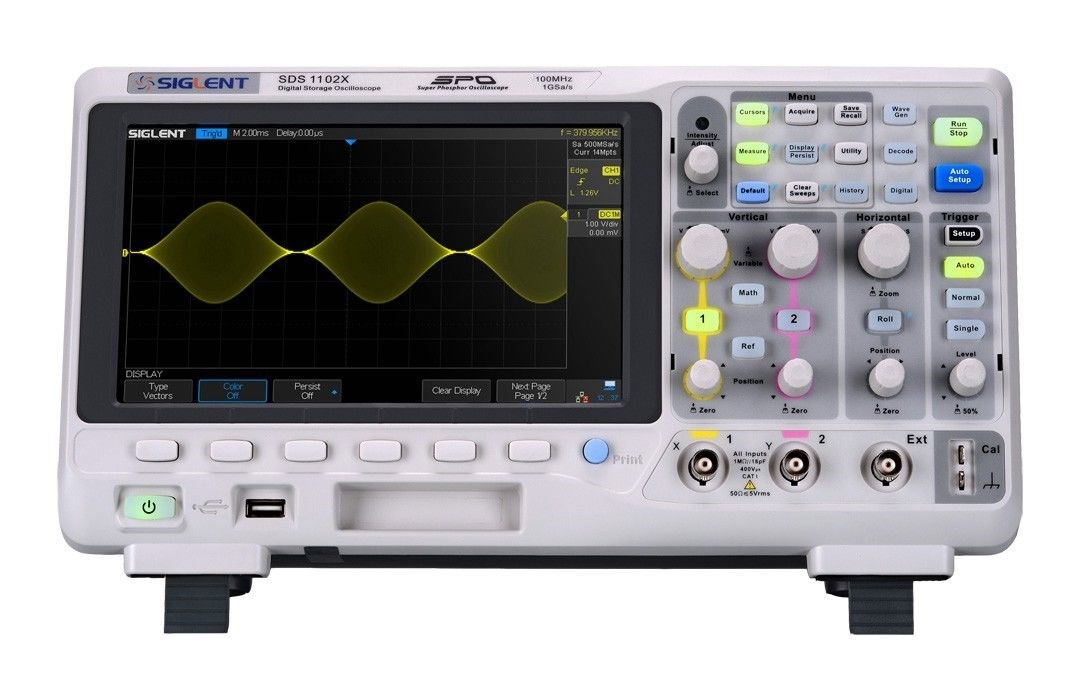
\includegraphics[width=.4\linewidth]{img/intro/digital_os}
    \caption{Digital oscilloscope}
\end{figure}
\subsubsection*{Analog sampling oscilloscopes}
An analog oscilloscope consists of a cathode ray tube (CRT), sweep generator and a vertical amplifier. The sweep generator causes an electron beam in the CRT to sweep horizontally across a phosphorescent screen. The vertical amplifier moves the beam in a vertical direction in response to an applied input signal. The horizontal and vertical movement of the electron beam traces out the input signal's time variations. This trace appears on the oscilloscope's screen.
\begin{figure}[H]
    \centering
    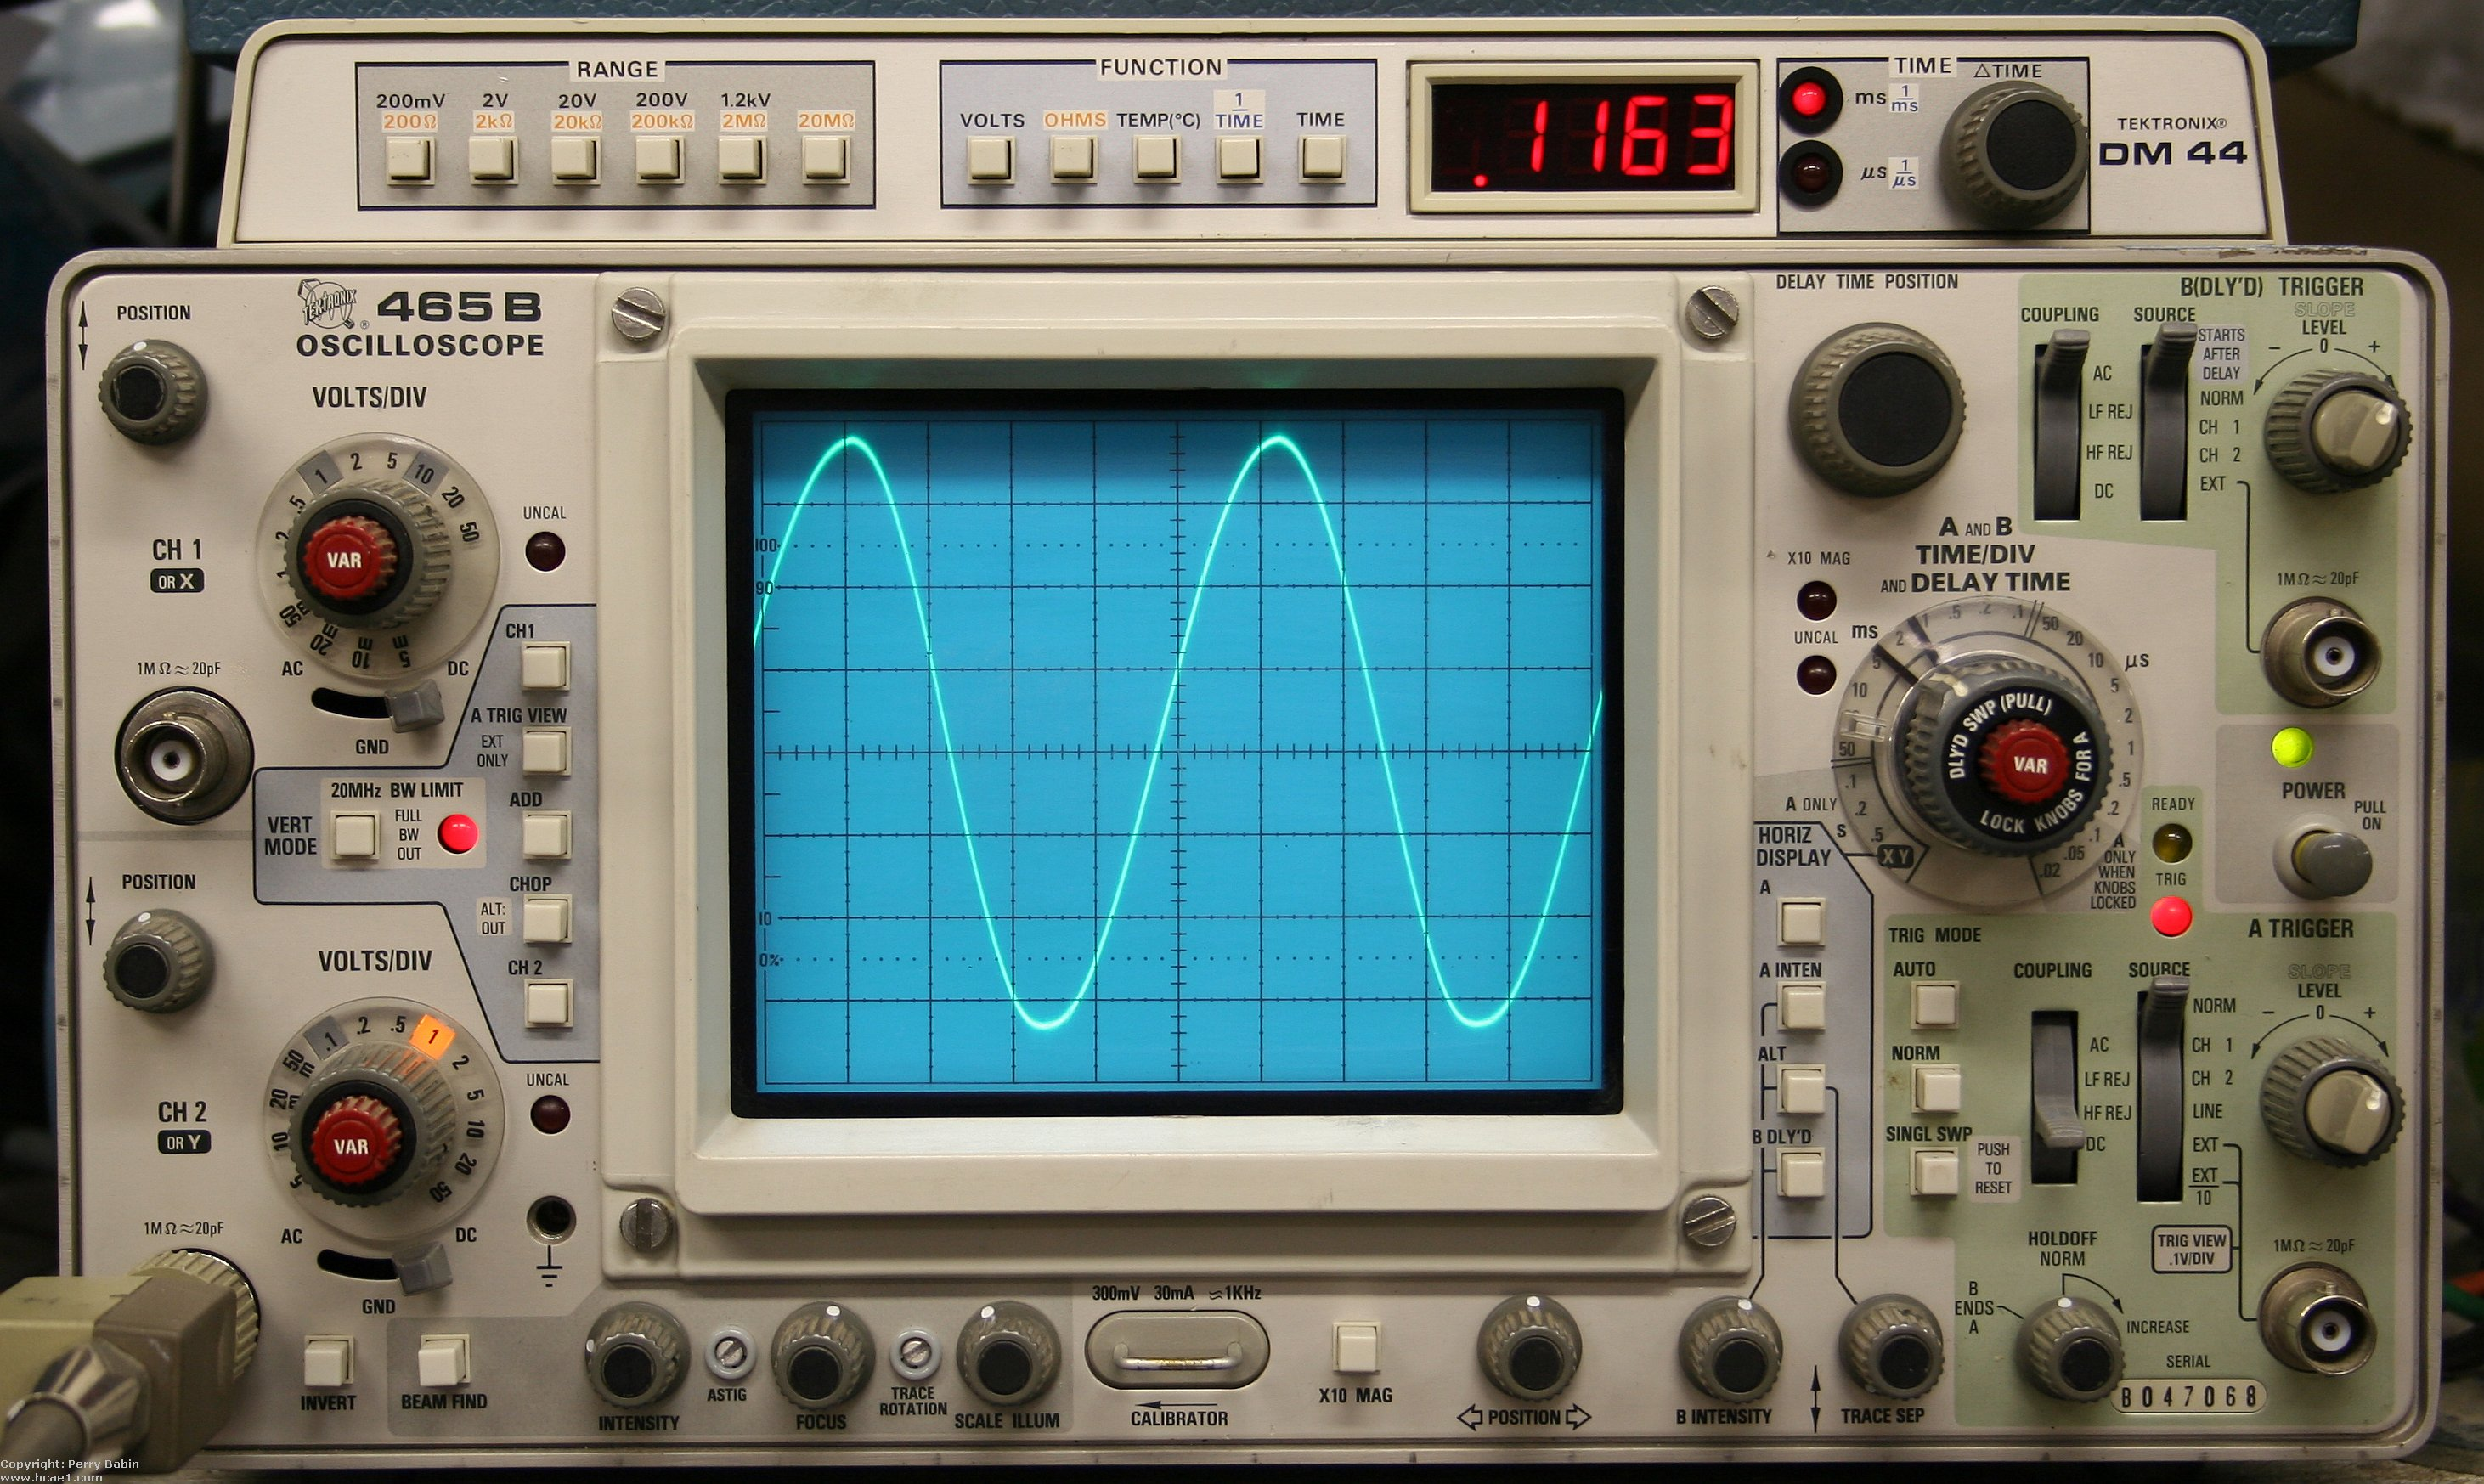
\includegraphics[width=.4\linewidth]{img/intro/analog_os}
    \caption{Analog oscilloscope}
\end{figure}
\subsubsection*{Handheld oscilloscopes}
Portable oscilloscopes are used in many field troubleshooting applications from electrical and electro-mechanical to electronic and industrial control systems. Usually this kind of oscilloscope tries to keep the characteristics of an efficient and comfortable device to use in any sort of situation.
\begin{figure}[H]
    \centering
    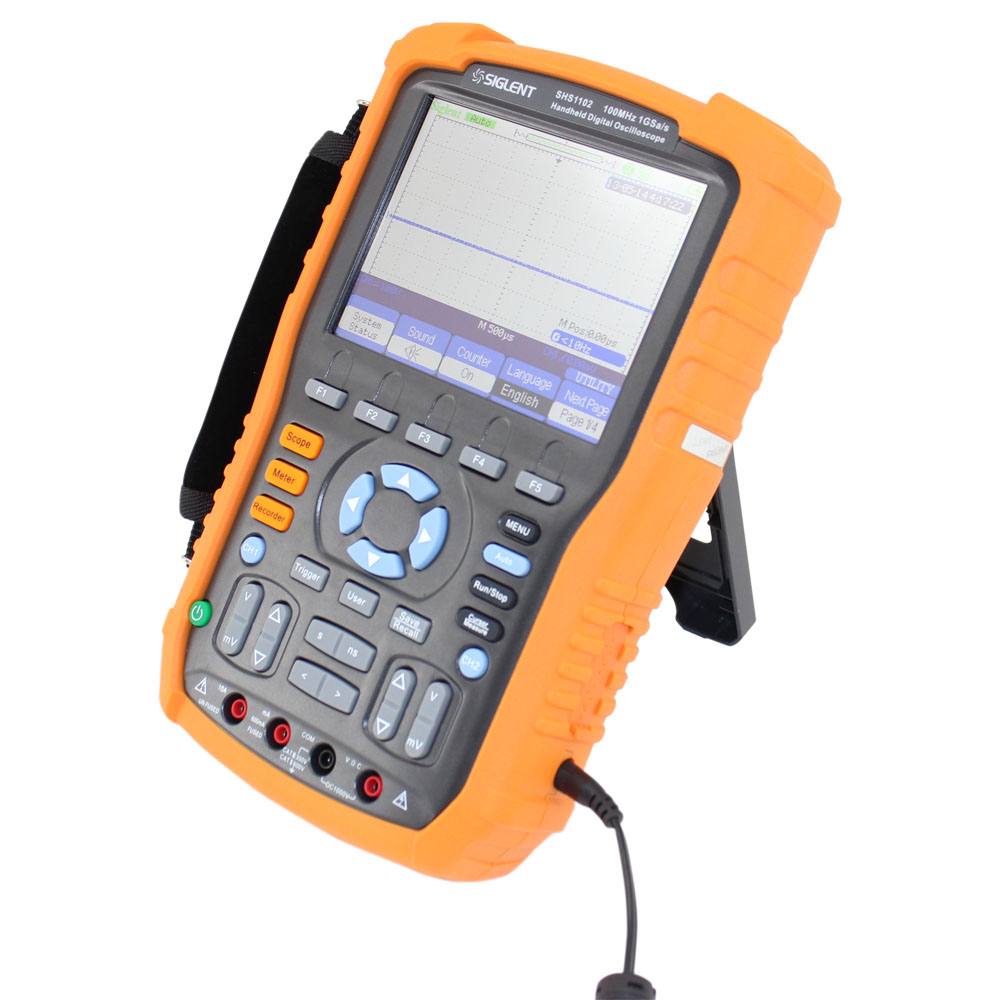
\includegraphics[width=.4\linewidth]{img/intro/hand_os}
    \caption{Analog oscilloscope}
\end{figure}

The difference in parameters such as sampling rates, memory depth, number of channels, probe requirement, bandwidth and analysis capability determines which oscilloscope is best suited for a given environment. Oscilloscopes have three major components: an electron gun, horizontal and vertical deflecting plates and a phosphor screen. A steady stream of electrons are provided by the electron gun, which moves in a constant direction. The electrons pass through the horizontal and vertical deflecting plates and the resulting electric field deflects the electrons to move vertically or horizontally. The electron beam thus produced hits the phosphor screen and produces a display on the monitor of the oscilloscope. A traditional oscilloscope works in almost exactly the same way as a traditional (cathode-ray tube) television; indeed, you'll sometimes see oscilloscopes referred to as cathode-ray oscilloscopes or CROs. In a TV, electron beams are made to scan back and forth across a screen coated on the back with special chemicals called phosphors. Each time the beam hits the screen, it makes the phosphors light up. In less time than it takes to blink an eye, the electron beams sweep across the entire screen and build up the picture you can see. Then they do it all over again. And again. And again. So you see a moving picture instead of a still one. (Take a quick look at our television article for a diagram showing you how all this works in practice.) In an oscilloscope, the electron beams work the same way but instead of building up a picture they draw a graph. When you watch a line being drawn on an oscilloscope screen, what you're actually looking at is an electron beam wobbling up and down.
Here’s an image to explain it better:     
\begin{figure}[H]
    \centering
    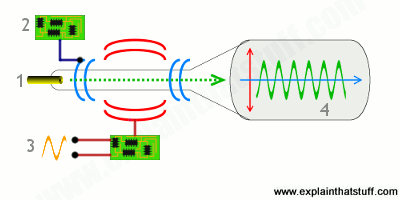
\includegraphics[width=.5\linewidth]{img/intro/how-works}
    \caption{\textit{
1) Inside the cathode-ray tube (CRT), the electron gun (yellow) fires a beam of electrons (green dots) toward the phosphor screen. 2) With no signal connected to the scope, a timing circuit powers electromagnet coils (blue) that make the electron beam sweep slowly across the screen from left to right (effectively powering the x-axis of the graph). 3) When you feed an undulating signal (orange) into the oscilloscope's probes, a different circuit powers a perpendicular pair of coils (red) that make the beam sweep up and down. 4) Acting together, the coils make the electron beams sweep out an up-and-down, wiggling trace (a sine wave).
}}
\end{figure}

    Oscilloscopes can measure the frequency and amplitude of a signal, as well as display the shape of the signal formed. It also provides all qualitative and quantitative information on time interval, rise time and distortion of the signal formed. The real-time analysis that can be provided is mostly useful for diagnostics. On-electrical signals like audio can be converted to voltages and observed on an oscilloscope. Adjustment is possible with knobs and controls found on the front panel. 
However, as they are designed primarily for waveform observation, oscilloscopes are less accurate than other testing devices to measure direct current voltages. Compared to other electronic and electrical measuring devices, oscilloscopes are costly and sophisticated. 
\newpage
\section{Development}
\subsection{Measurement of the test signal}
In the first part of the experiment we connected a pair of test leads to each of the outputs in the
oscilloscope, then we clipped the probes connected to the channel one (CH1) to the test output,
at this point we could see a flat and thin yellow line along the display, then, using the knobs to
adjust the relation between volts per division and seconds per division displayed in the grid until we could see,
according to the label in the oscilloscope, a clear square wave with the volts per division
set at \SI{5}{\volt} and the frequency at \SI{300}{\hertz}. Afterwards we proceed in the same
way, now using the leads connected in channel two (CH2).
\subsubsection{Measurements}
For channel 1(CH1) we have:
\begin{gather*}
    Time/div = \SI{500}{\micro\second}/div\\
    Volts/div = \SI{4.84}{\volt}/div
\end{gather*}
For channel 2(CH2) we have:
\begin{gather*}
    Time/div = \SI{500}{\micro\second}/div\\
    Volts/div = \SI{5}{\volt}/div
\end{gather*}
If period($T$) is given by:
\[T = \frac{time}{div}\times Number\ of\ horizontal\ divisions\]
the period($T$) for channel 1(CH1) is:
\[T_1 = \SI{500}{\micro\second}\times10\qquad\therefore T_1 = \num{5e-3}\si{\second}\ (\SI{5}{\milli\second})\]
the period($T$) for channel 2(CH2) is:
\[T_2 = \SI{500}{\micro\second}\times10\qquad\therefore T_2 = \num{5e-3}\si{\second}\ (\SI{5}{\milli\second})\]

On the other hand, frequency($f$) is given by:
\[f = \frac{1}{T}\]
therefore, the frequency($f$) for channel 1(CH1) is:
\[f_1 = \frac{1}{T_1} = \frac{1}{\SI{500}{\micro\second}}\qquad \therefore f_1 = \SI{200}{\hertz}\]
the frequency($f$) for channel 2(CH2) is:
\[f_2 = \frac{1}{T_2} = \frac{1}{\SI{500}{\micro\second}}\qquad \therefore f_2 = \SI{200}{\hertz}\]

Peak-to-peak voltage($V_{pp}$) is given by:
\[V_{pp} = \frac{volts}{div}\times Number\ of\ vertical\ divisions\]
hence, the peak-to-peak voltage($V_{pp}$) for channel 1(CH1) is:
\[V_{pp1} = \SI{4.84}{\volt}\times8\qquad\therefore V_{pp1} = 38.72V_{pp}\]
also, the peak-to-peak voltage($V_{pp}$) for channel 2(CH2) is:
\[V_{pp2} = \SI{4.84}{\volt}\times8\qquad\therefore V_{pp2} = 40V_{pp}\]
\begin{figure}[H]
    \centering
    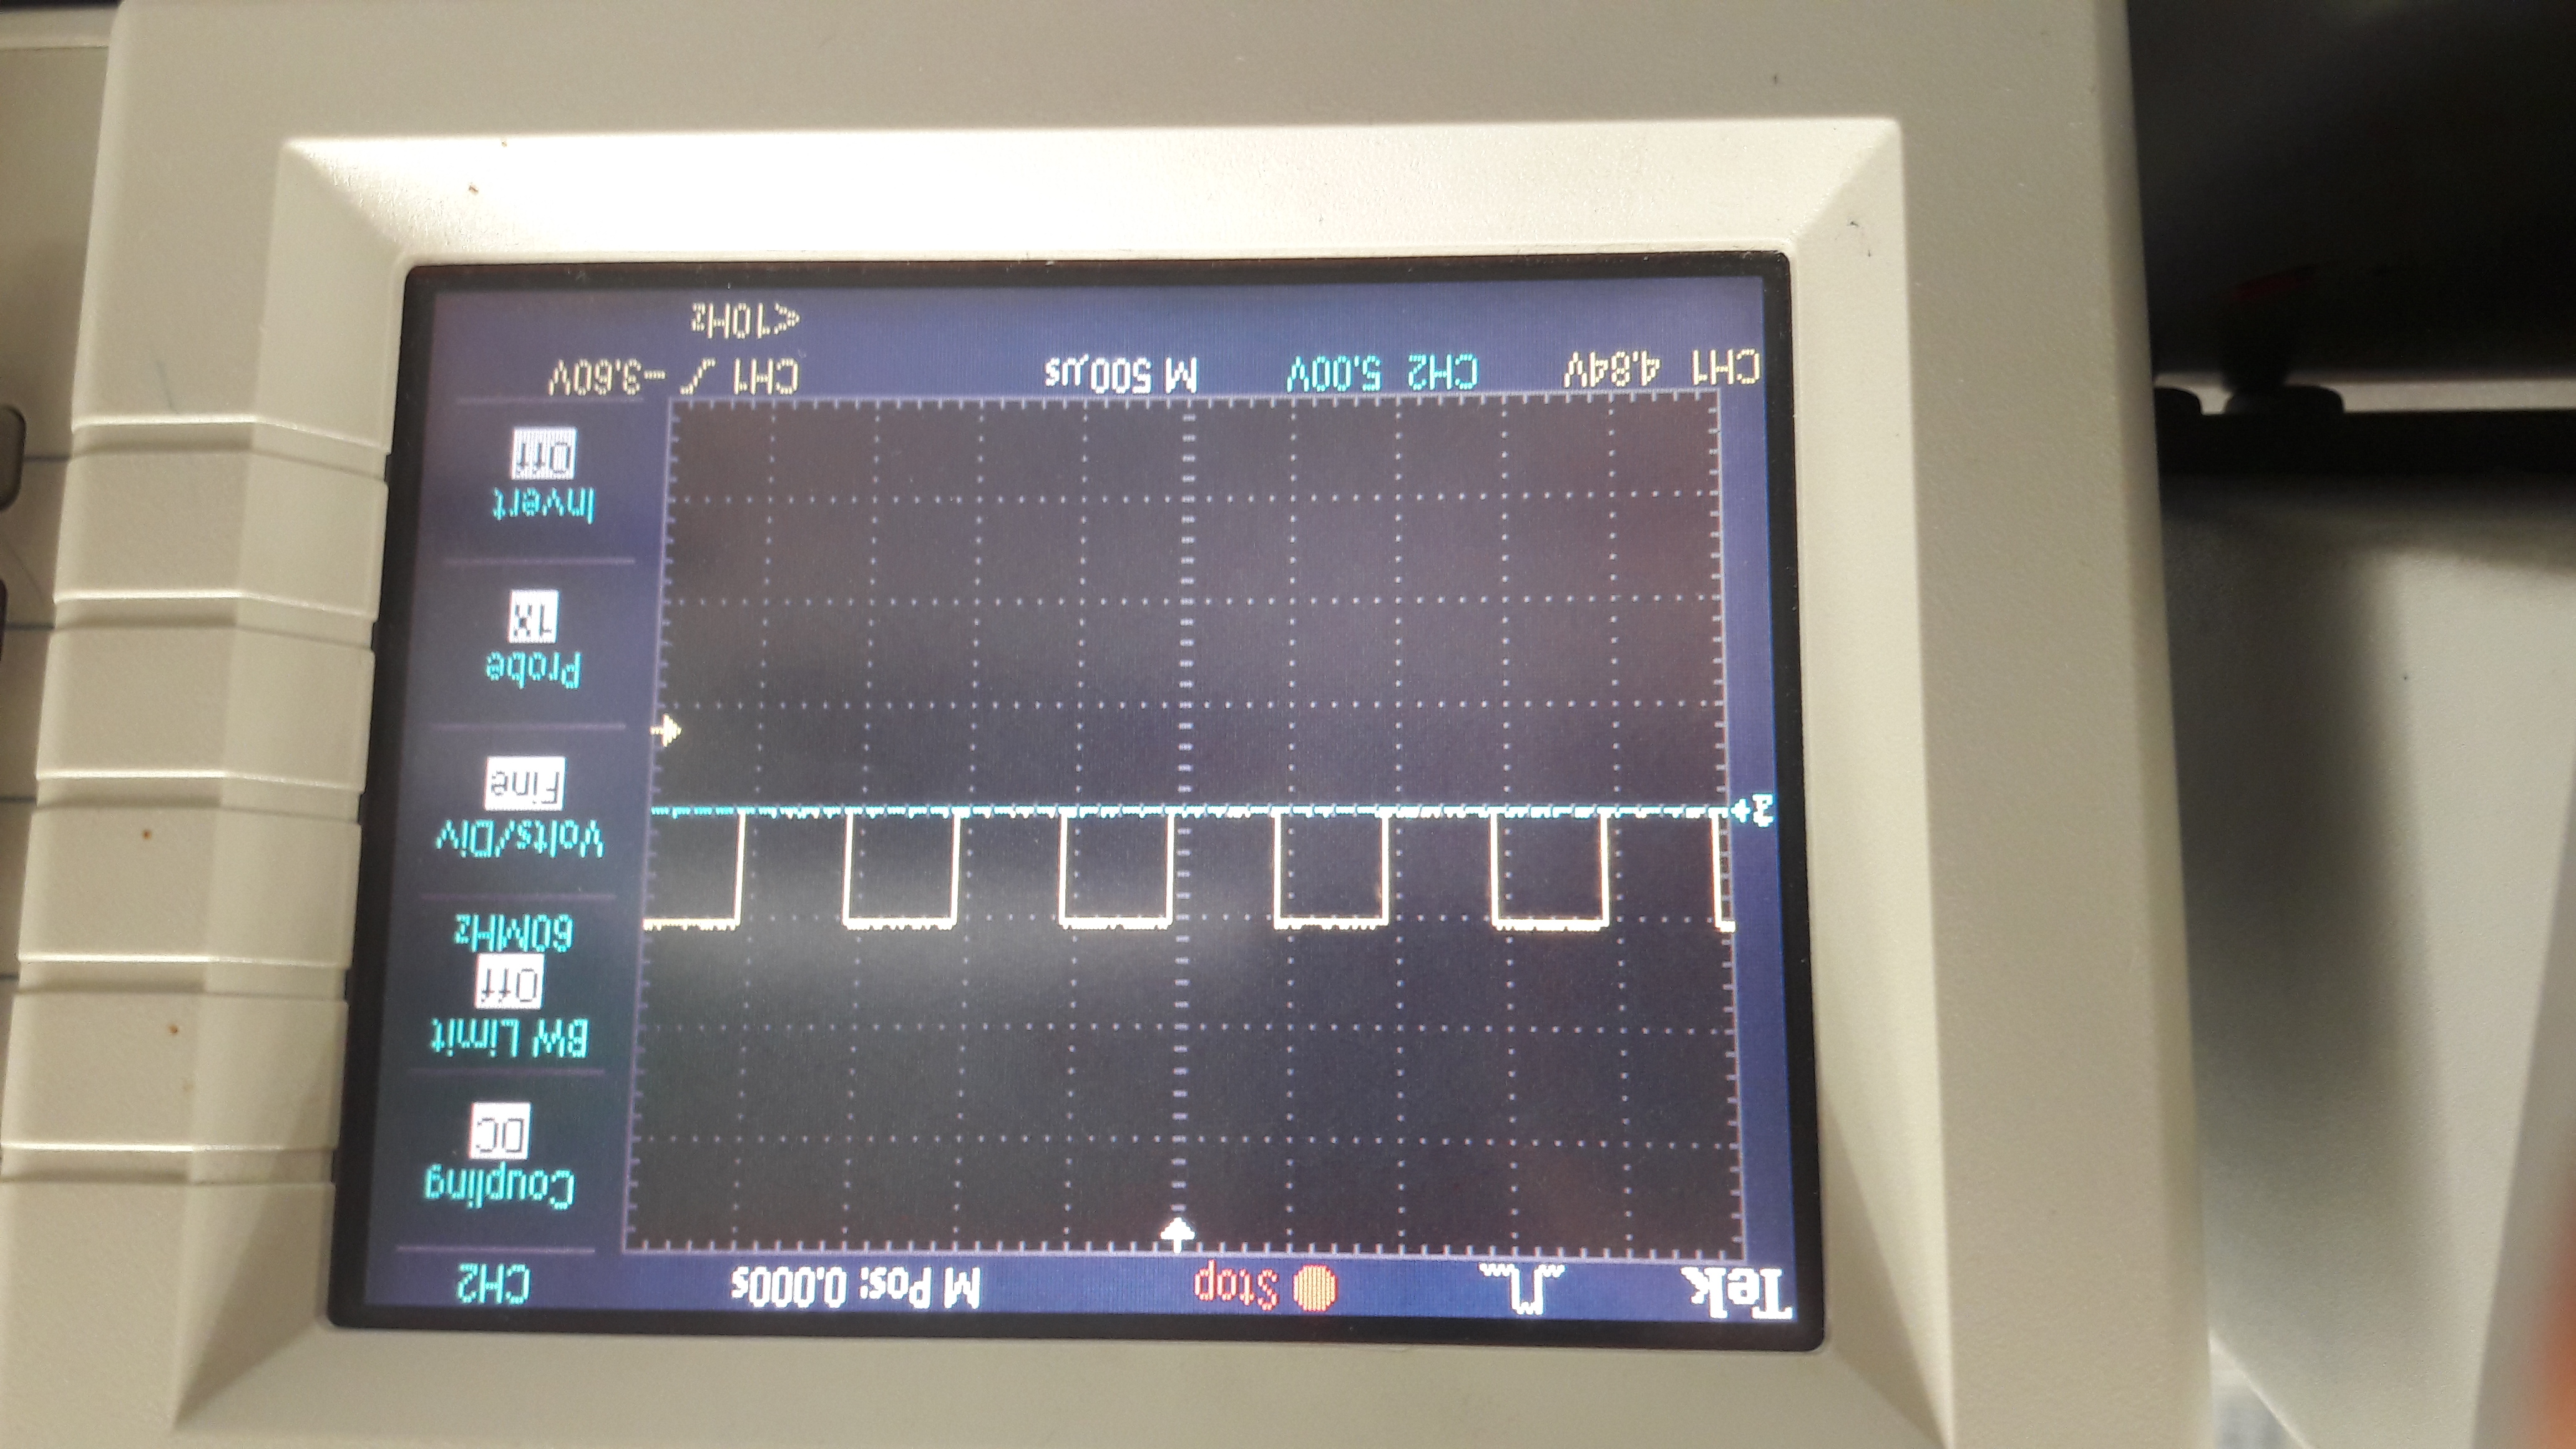
\includegraphics[width=.5\linewidth,angle=180]{img/part1/4}
    \caption{Oscilloscope showing the test signal on channel 2 (CH2)}
\end{figure}
\subsection{Testing the signal generator}
In the second part of the experiment we connected the signal generator to the oscilloscope and
set the generator to a frequency of \SI{10}{\kilo\hertz} and a frequency of $10 V_{pp}$,
alternating between the sine, triangular and squared wave.\\[2ex]
\subsubsection{Measurements}
{\textbf{Sine wave}}
\begin{gather*}
    Amplitude\ V_{pp}: \SI{5}{\volt}\\
    Period(T): \SI{100}{\micro\second}\\
    Frequence(f): \SI{10}{\kilo\hertz}
\end{gather*}
\begin{figure}[H]
    \begin{subfigure}{0.55\textwidth}
        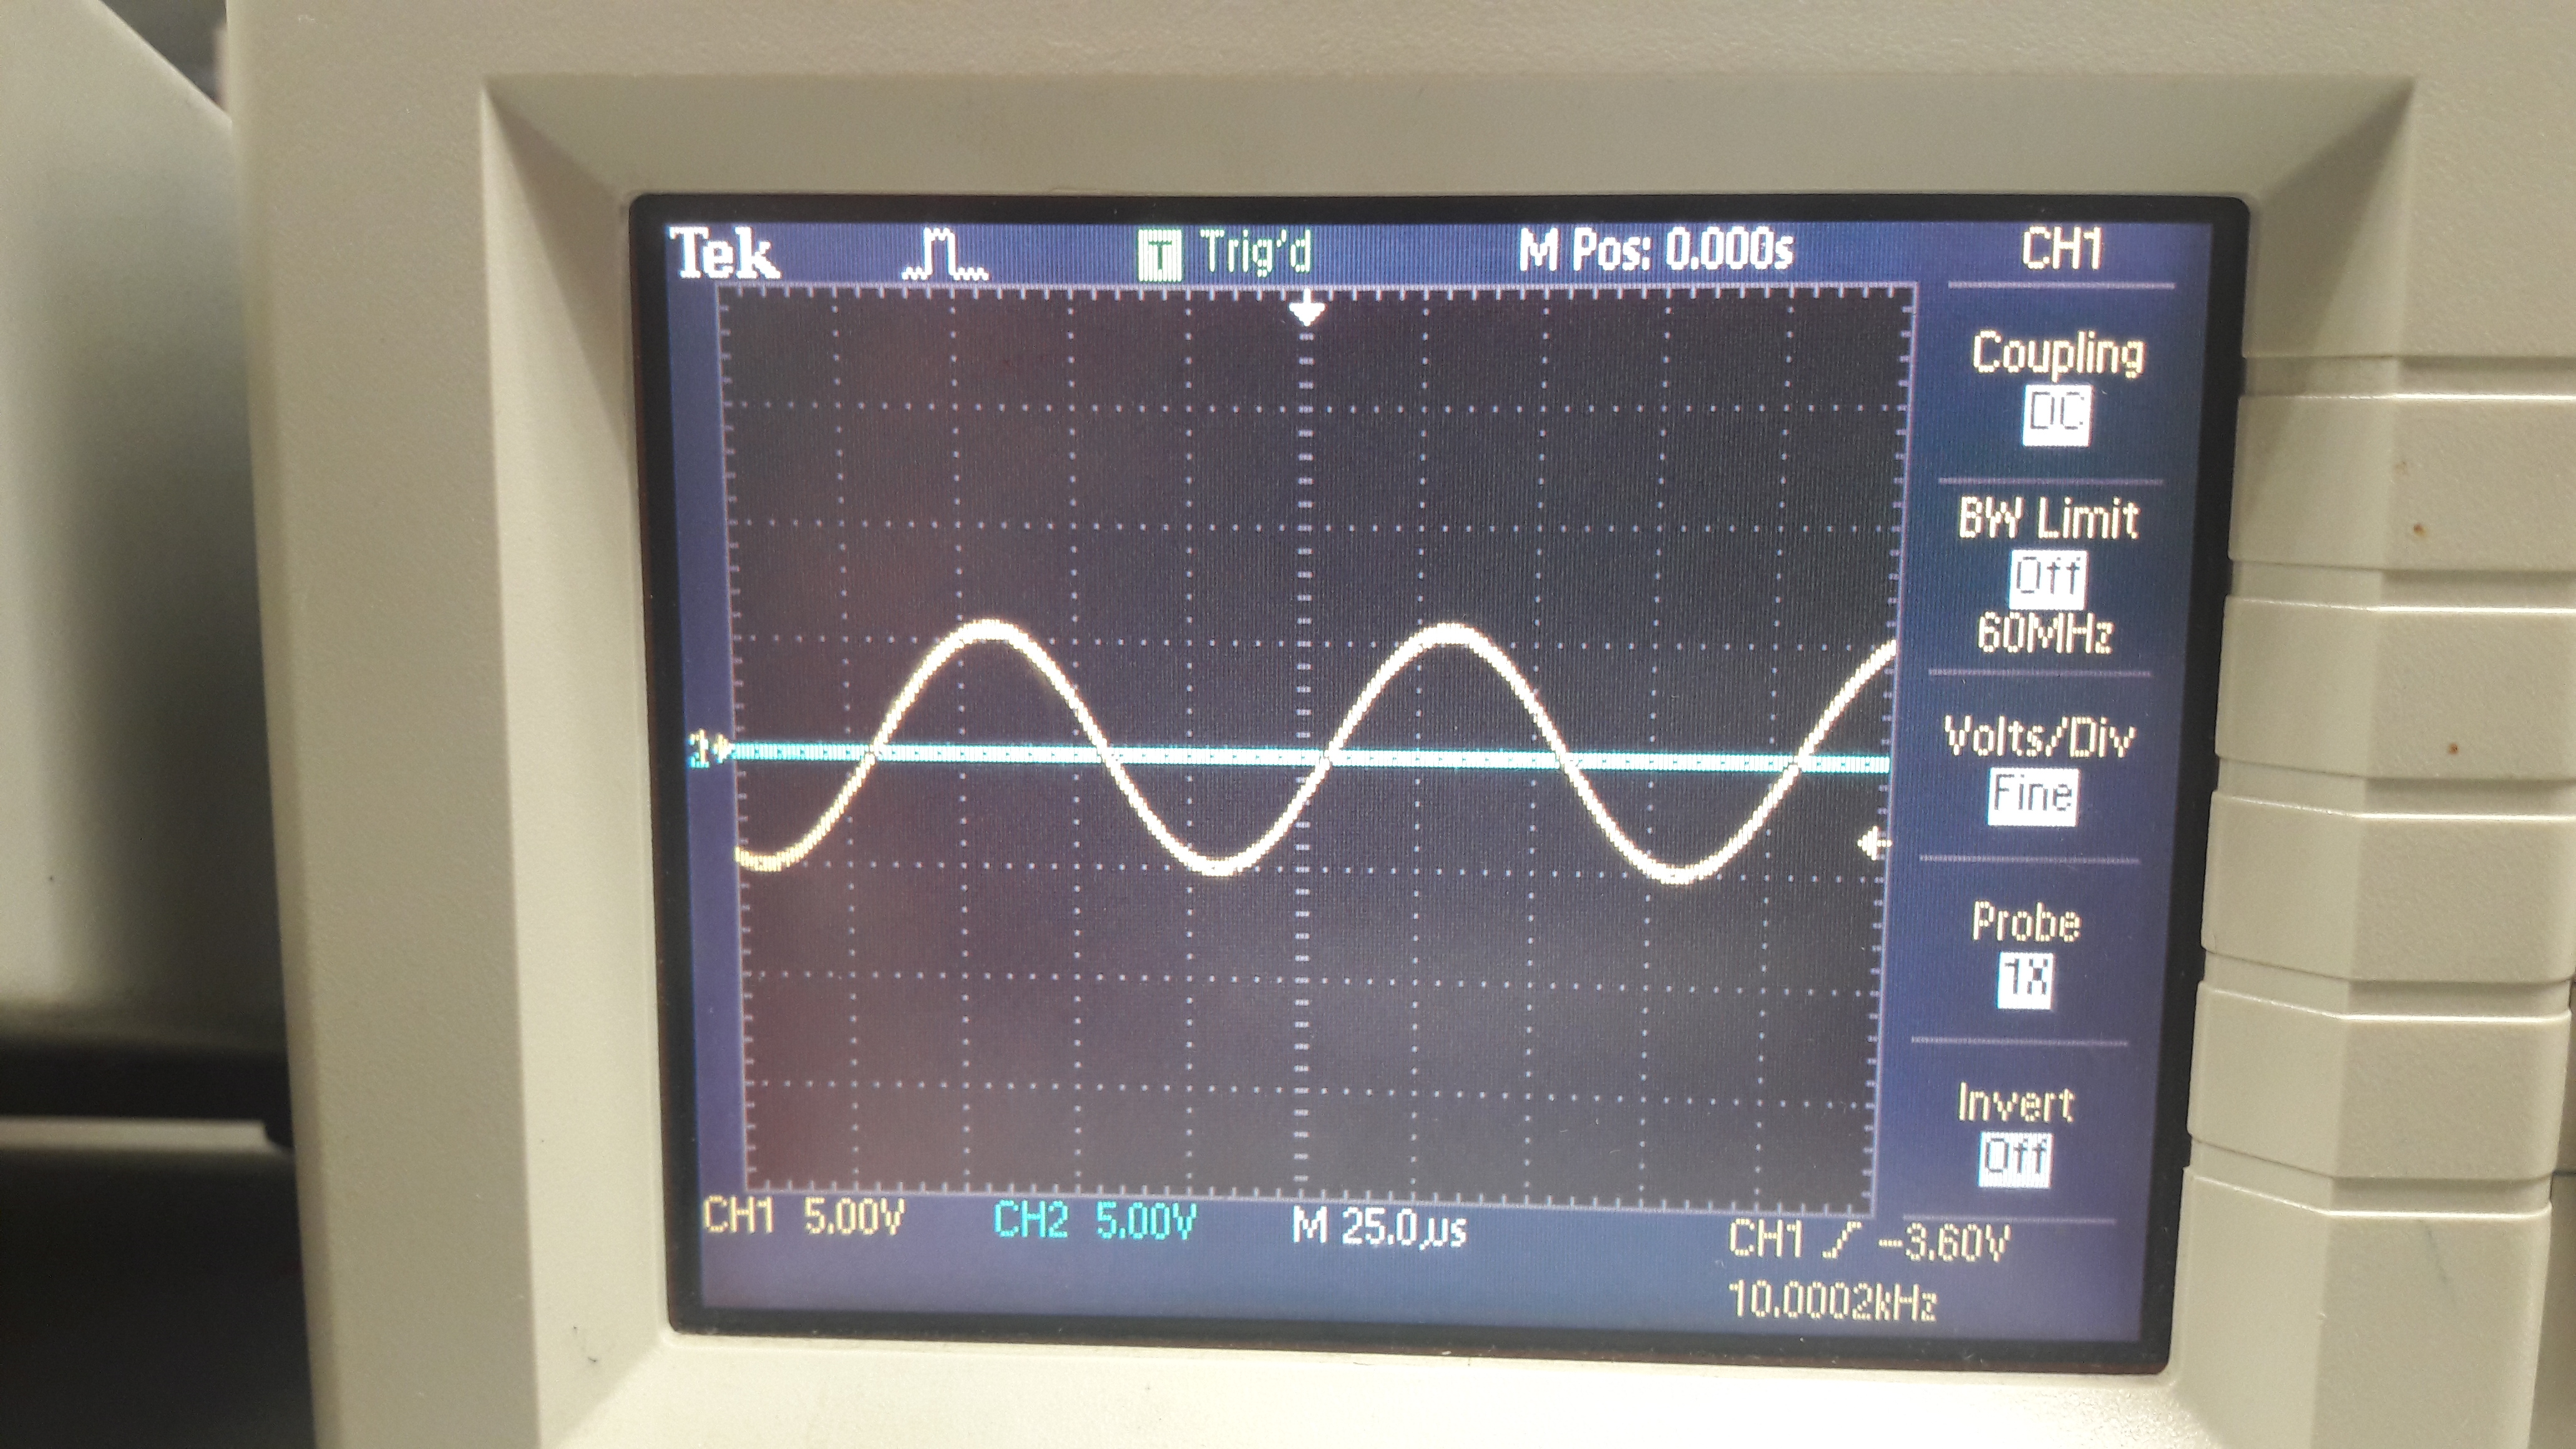
\includegraphics[width=.95\linewidth]{img/part2/1}
        \caption{Oscilloscope showing the sine wave}
    \end{subfigure}
    \begin{subfigure}{0.55\textwidth}
        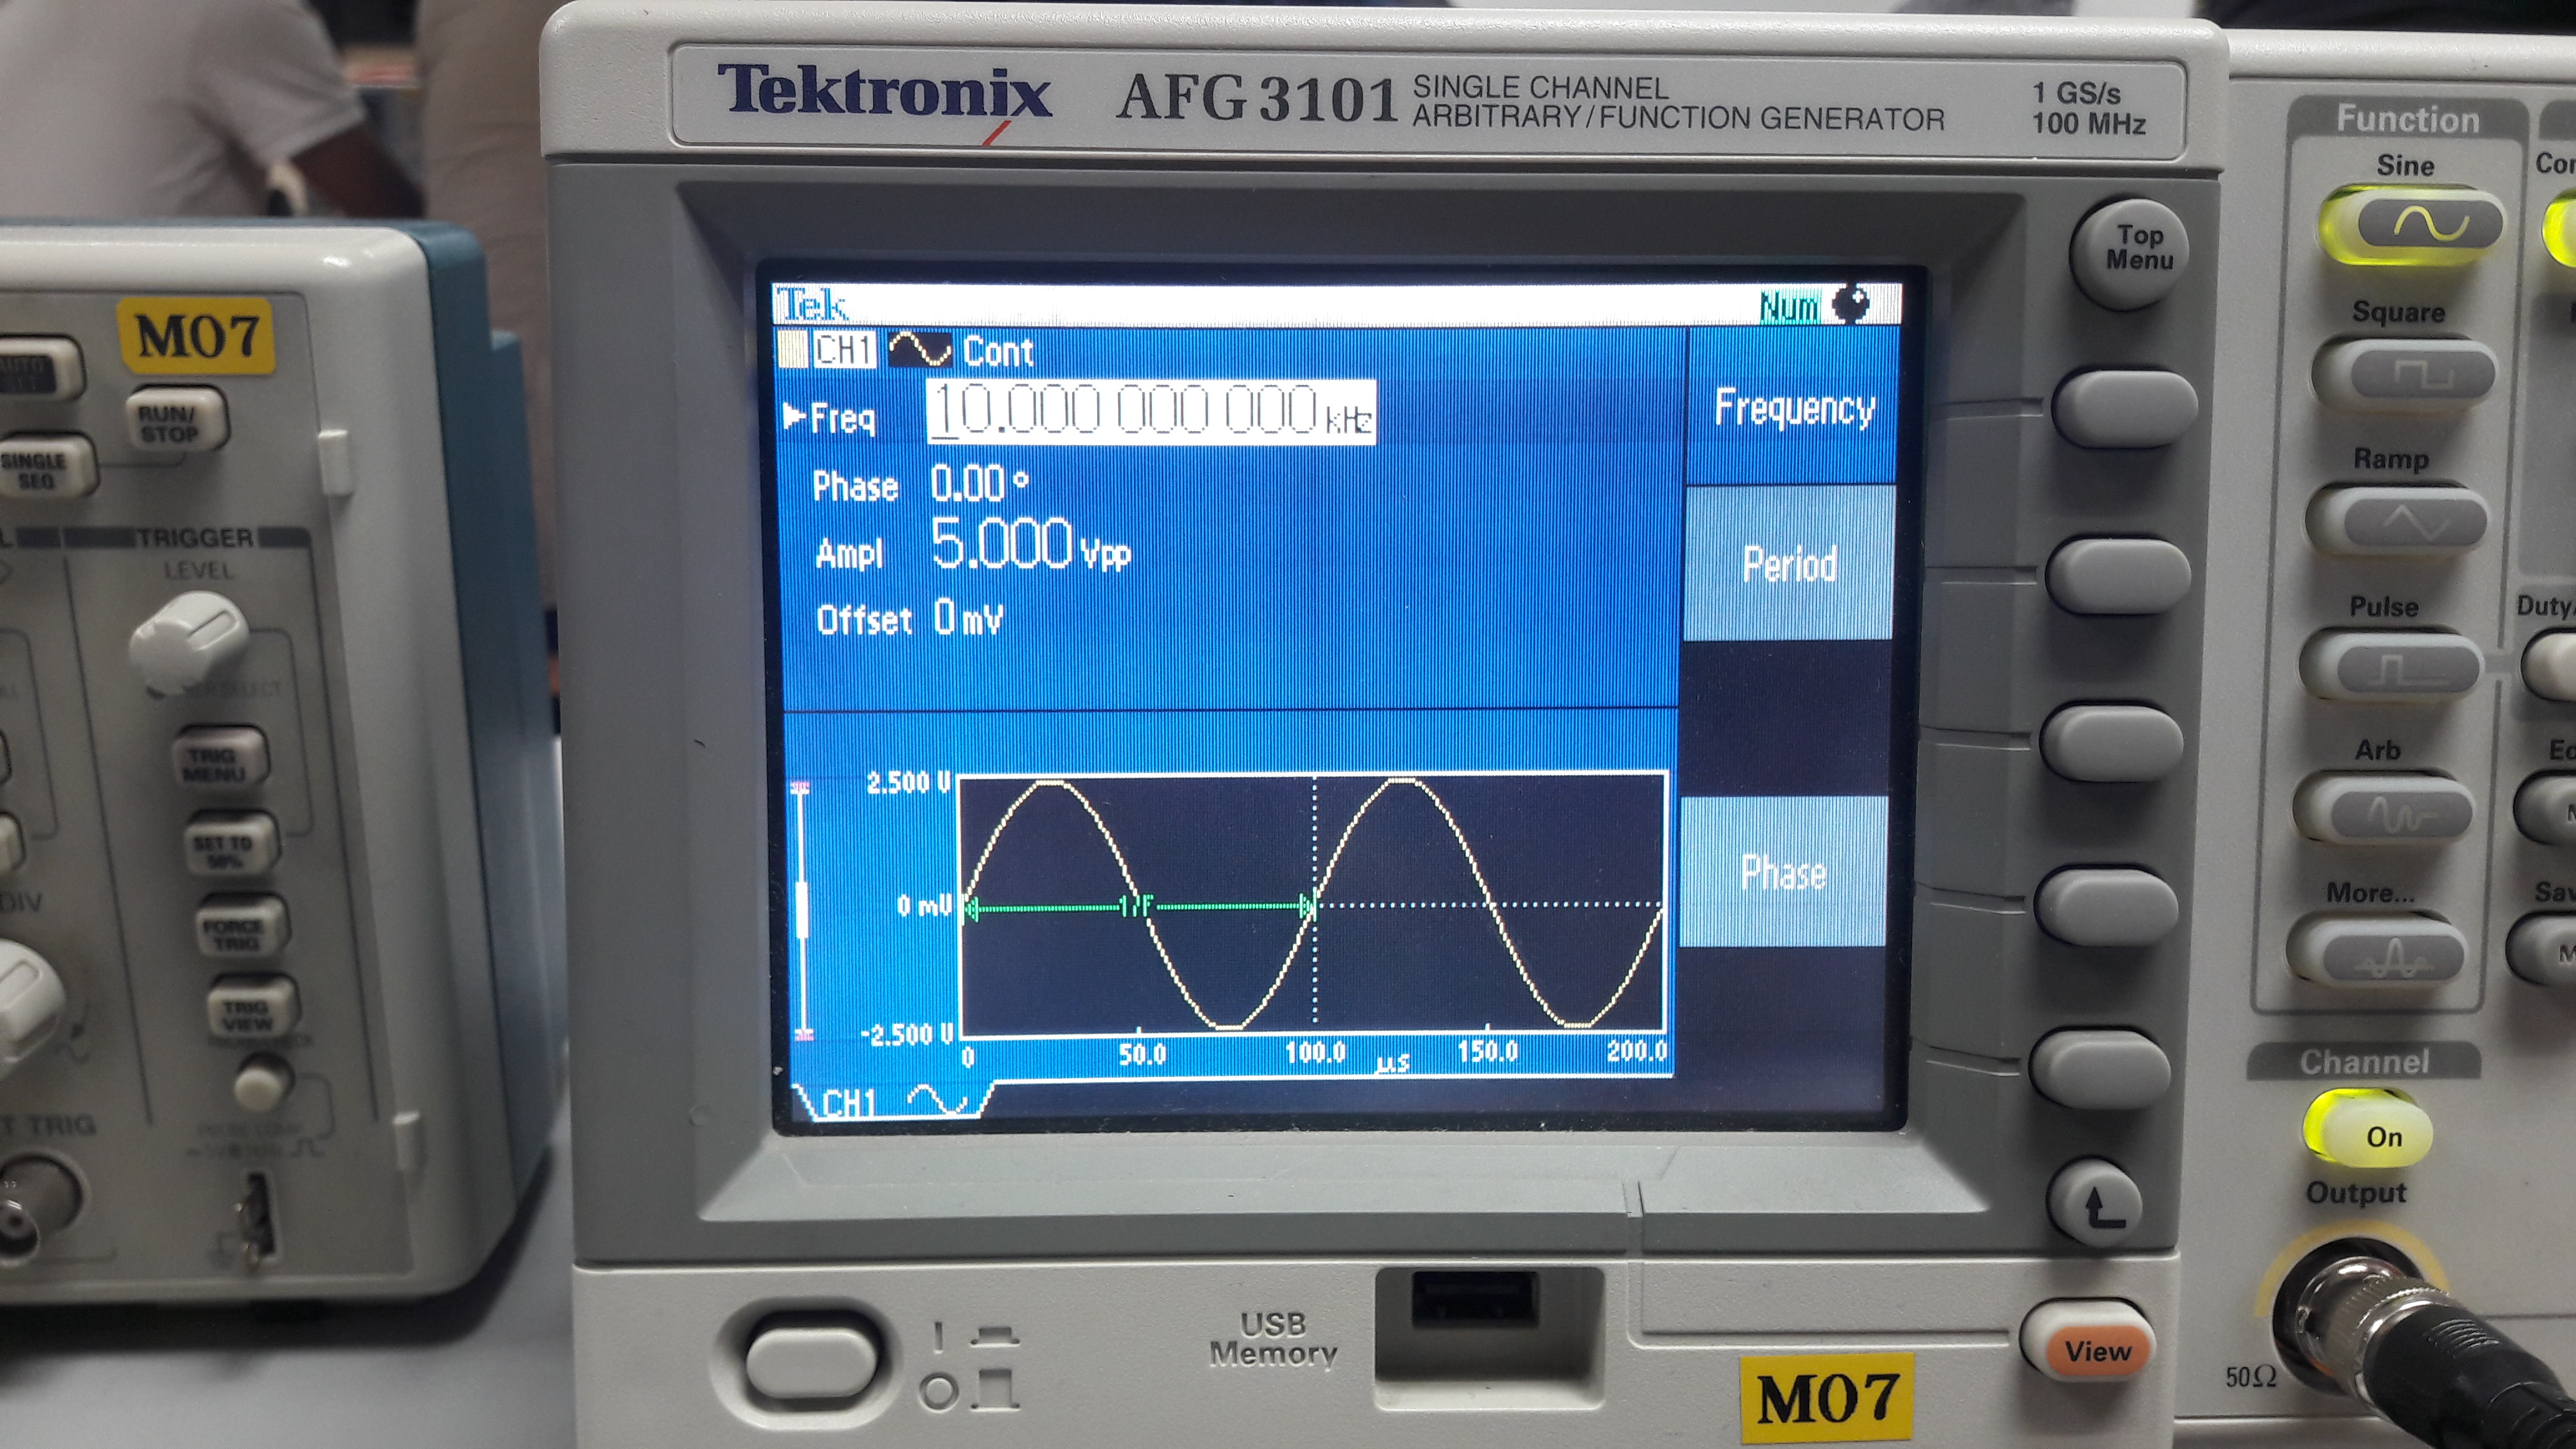
\includegraphics[width=.95\linewidth]{img/part2/2}
        \caption{Signal generator set to produce the sine wave}
    \end{subfigure}
    \caption{Sine wave generation and display}
\end{figure}
{\textbf{Triangular wave}}
\begin{gather*}
    Amplitude\ V_{pp}: \SI{5}{\volt}\\
    Period(T): \SI{100}{\micro\second}\\
    Frequence(f): \SI{10}{\kilo\hertz}
\end{gather*}
\begin{figure}[H]
    \begin{subfigure}{0.55\textwidth}
        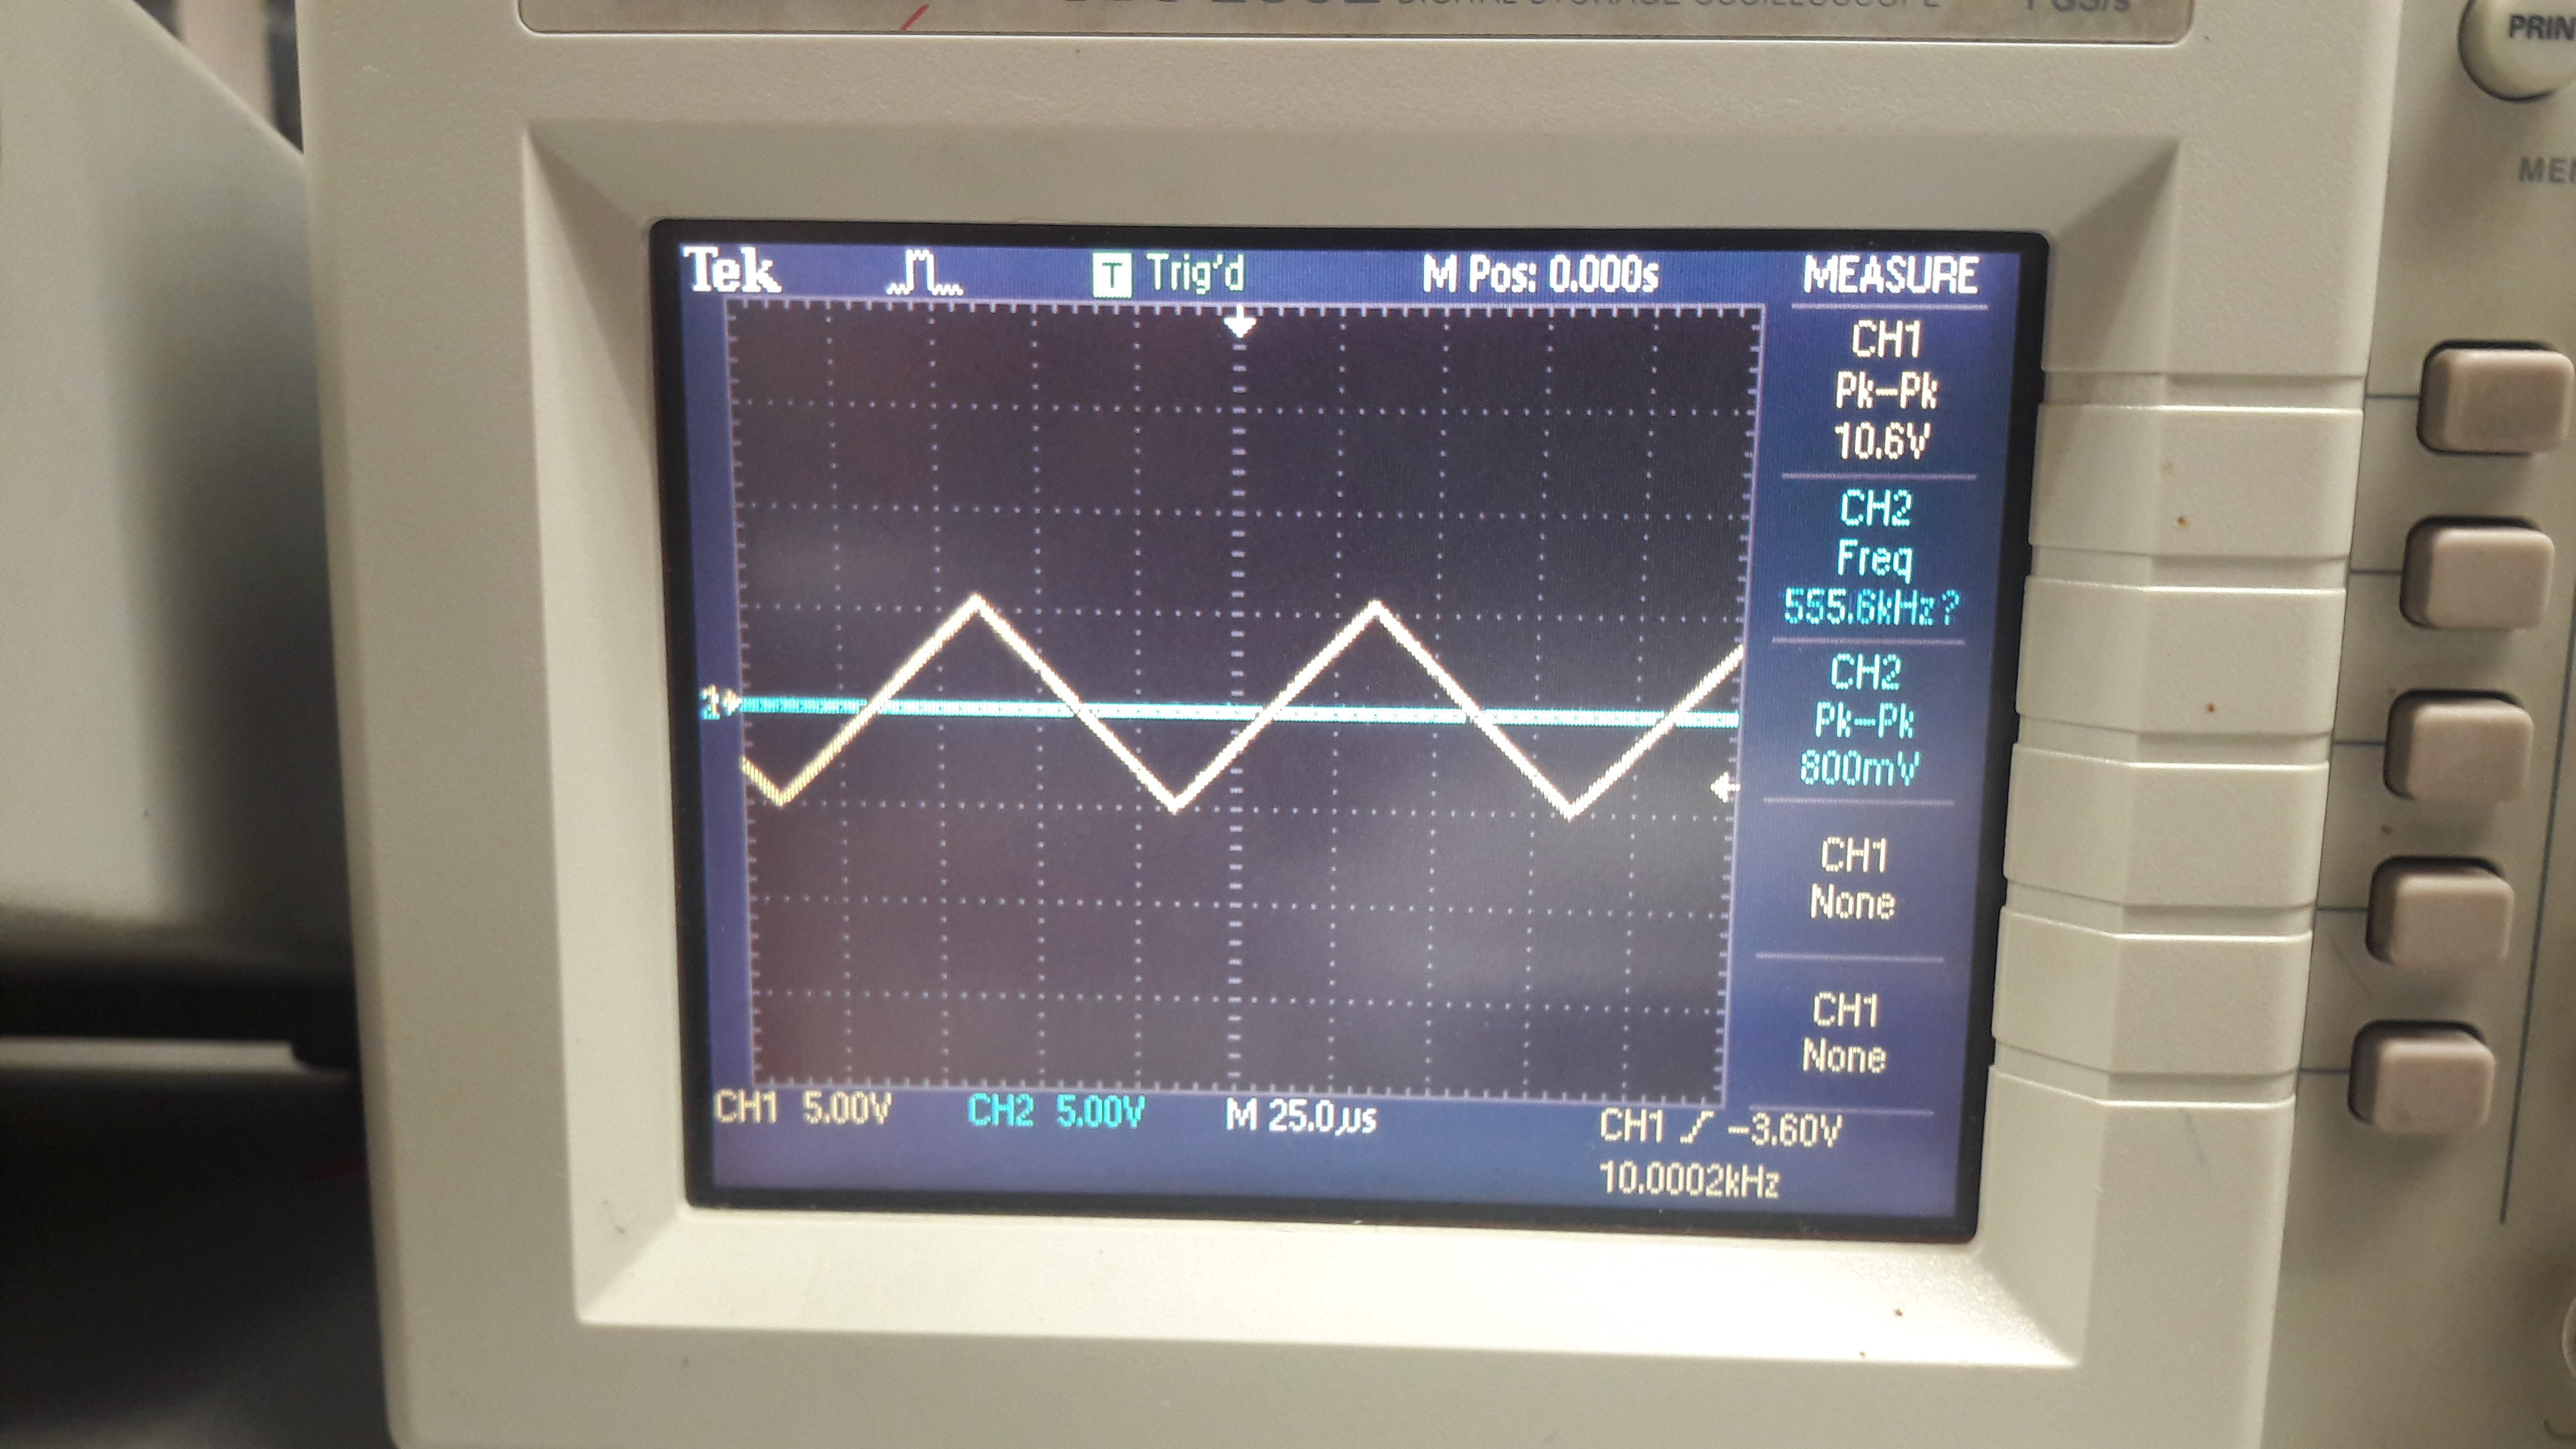
\includegraphics[width=.95\linewidth]{img/part2/7}
        \caption{Oscilloscope showing the triangular wave}
    \end{subfigure}
    \begin{subfigure}{0.55\textwidth}
        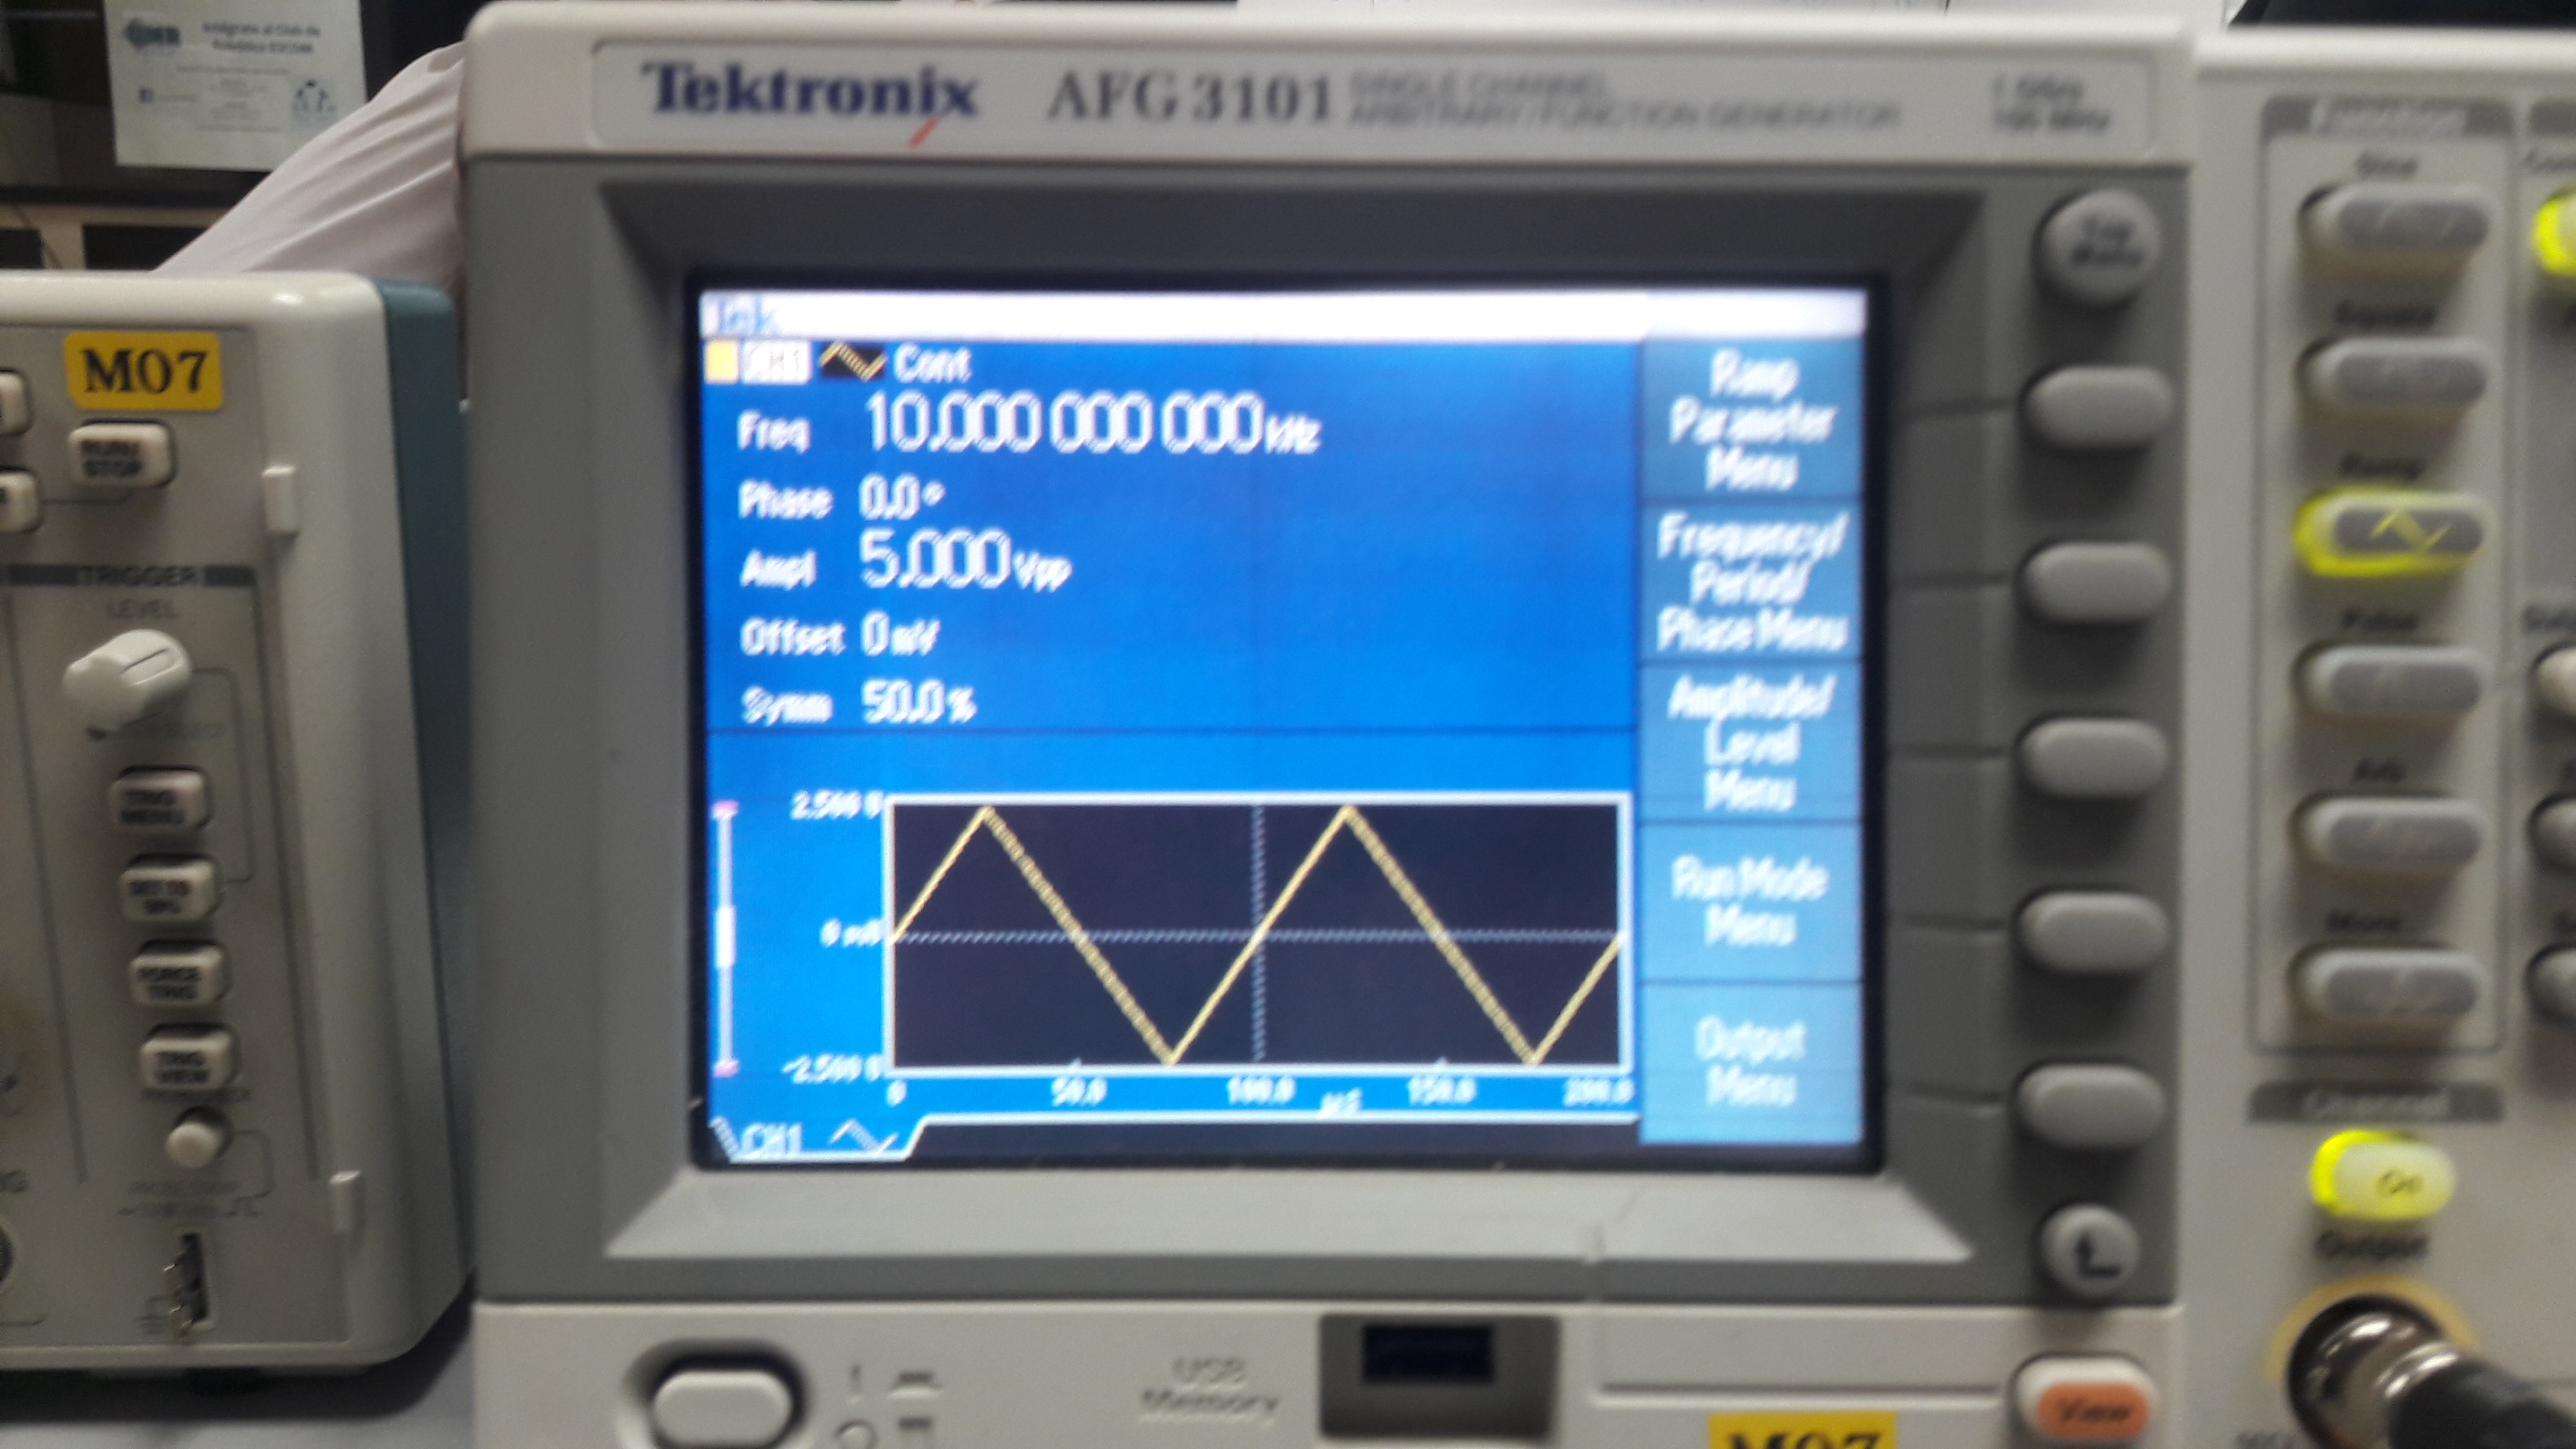
\includegraphics[width=.95\linewidth]{img/part2/5}
        \caption{Signal generator set to produce the triangular wave}
    \end{subfigure}
    \caption{Triangular wave generation and display}
\end{figure}
{\textbf{Square wave}}
\begin{gather*}
    Amplitude\ V_{pp}: \SI{5}{\volt}\\
    Period(T): \SI{100}{\micro\second}\\
    Frequence(f): \SI{10}{\kilo\hertz}
\end{gather*}
\begin{figure}[H]
    \begin{subfigure}{0.55\textwidth}
        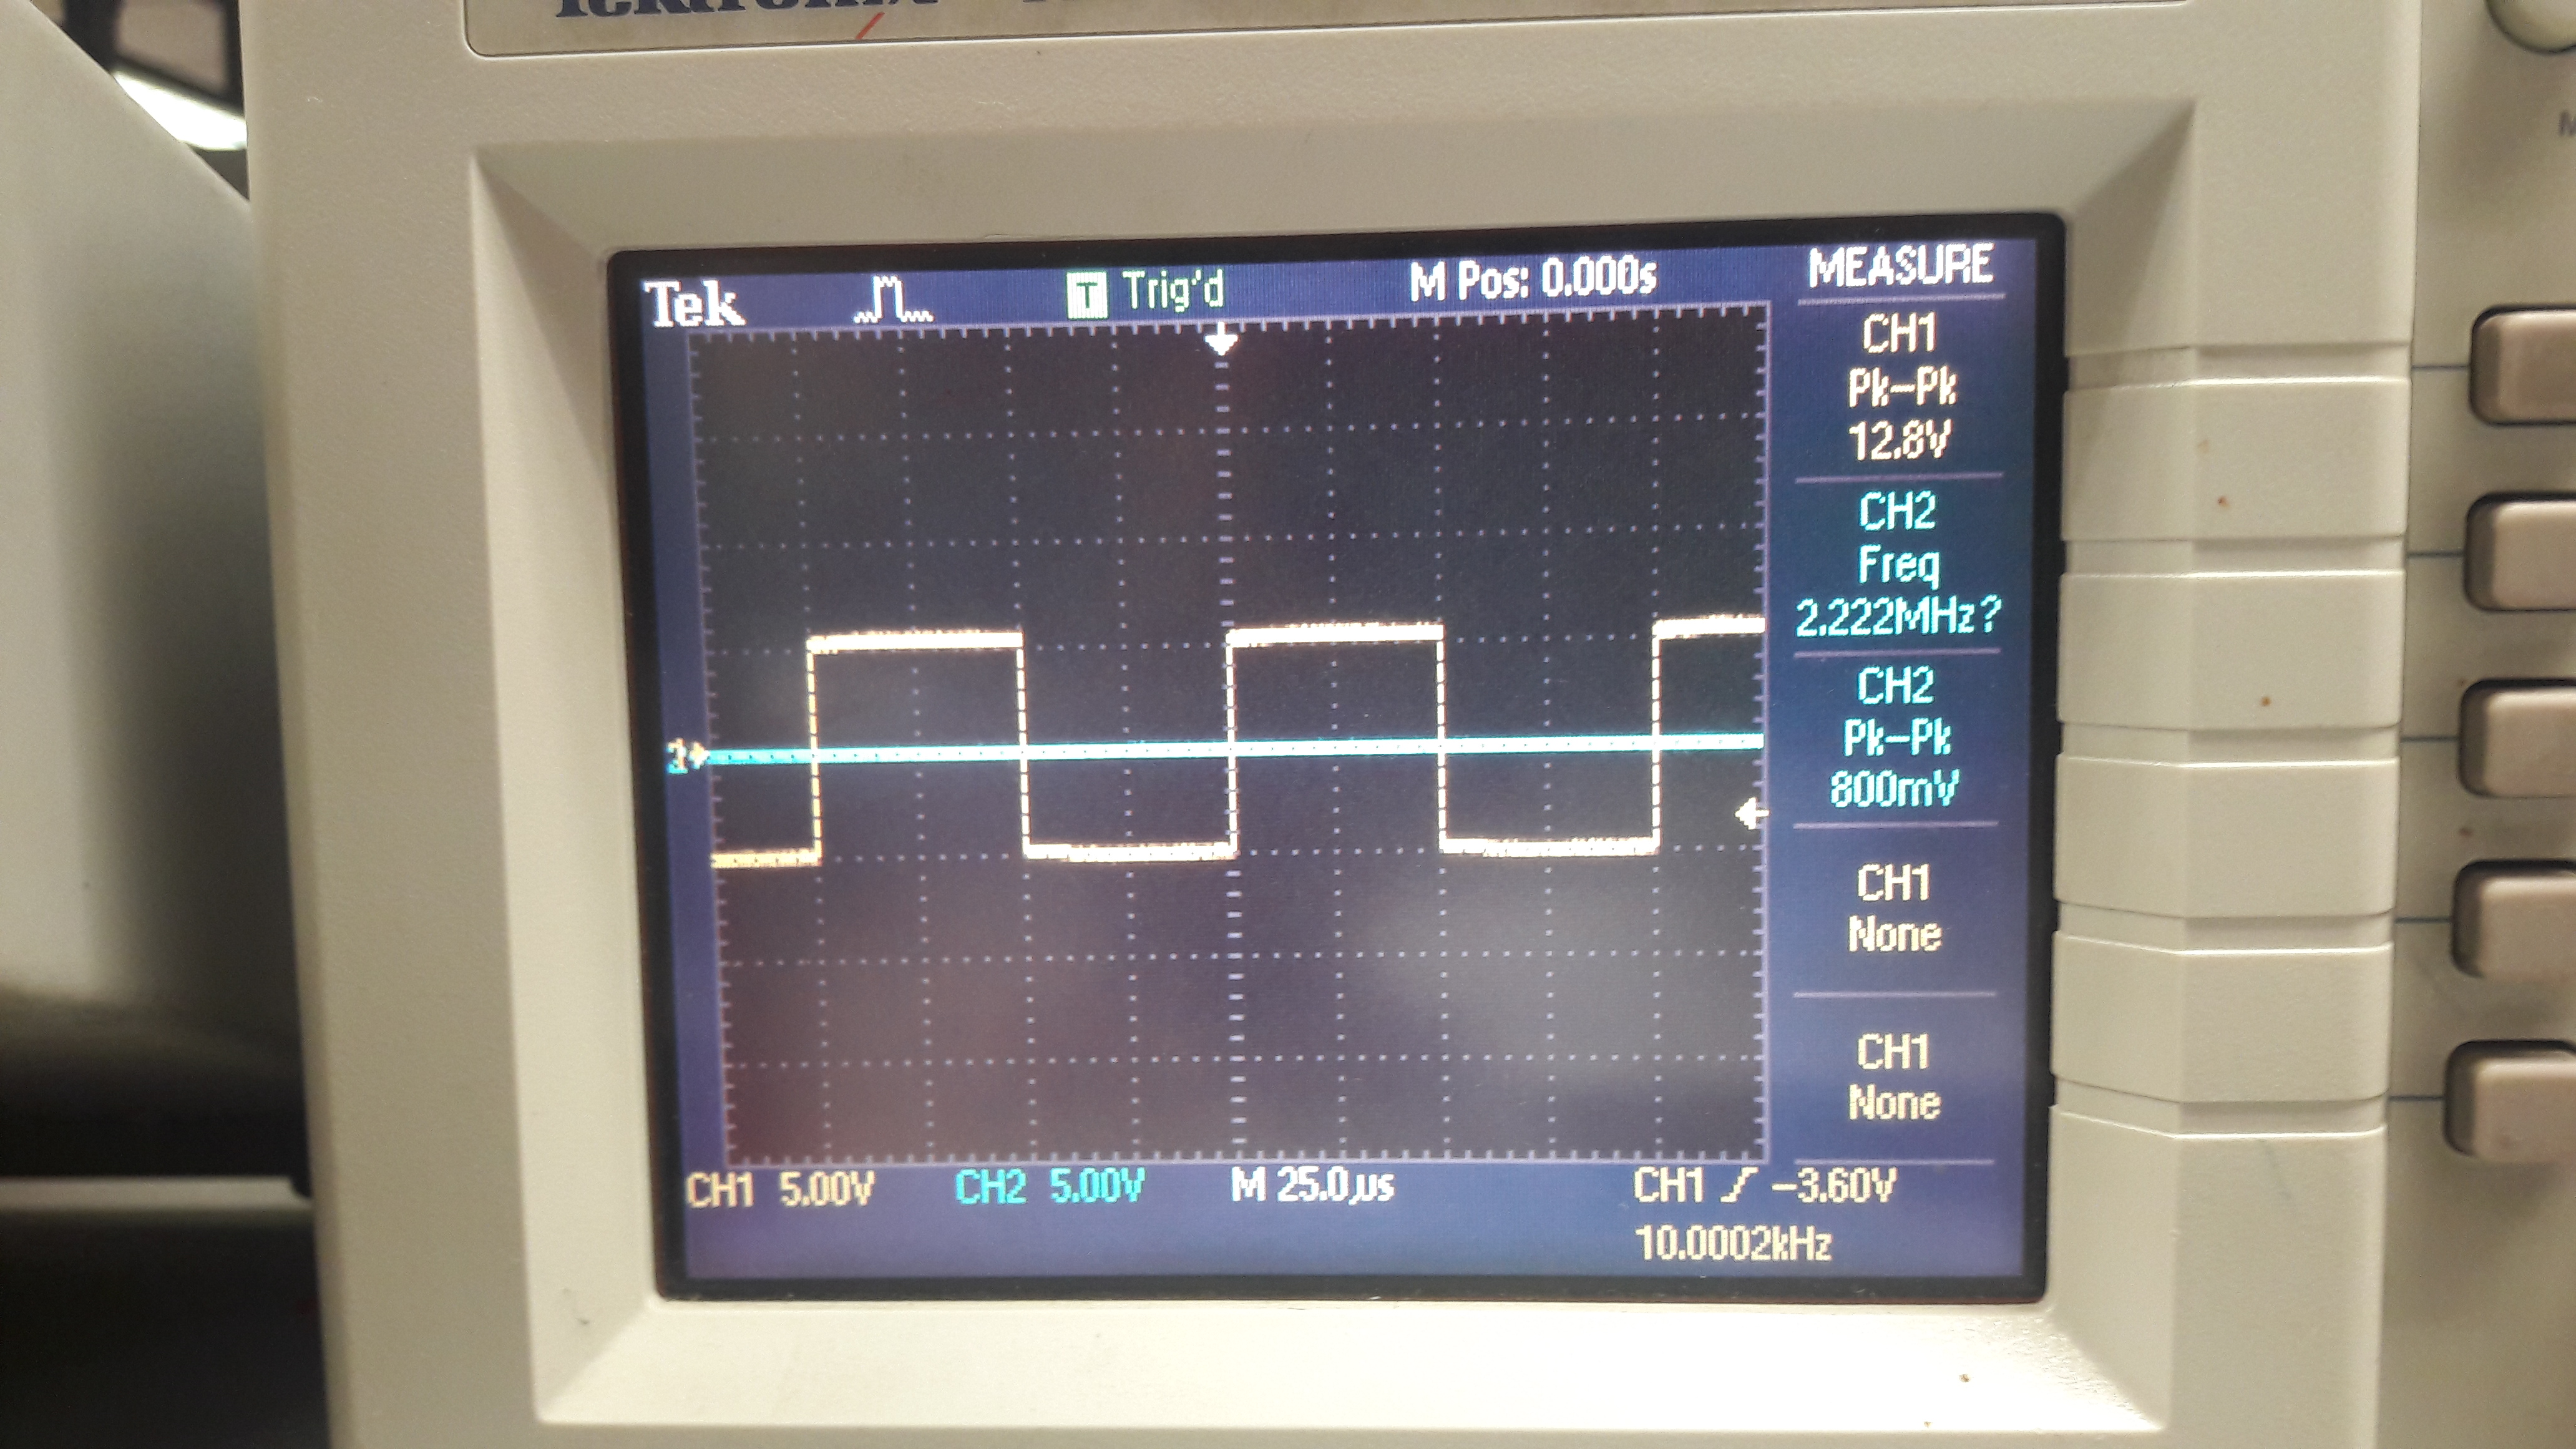
\includegraphics[width=.95\linewidth]{img/part2/11}
        \caption{Oscilloscope showing the square wave}
    \end{subfigure}
    \begin{subfigure}{0.55\textwidth}
        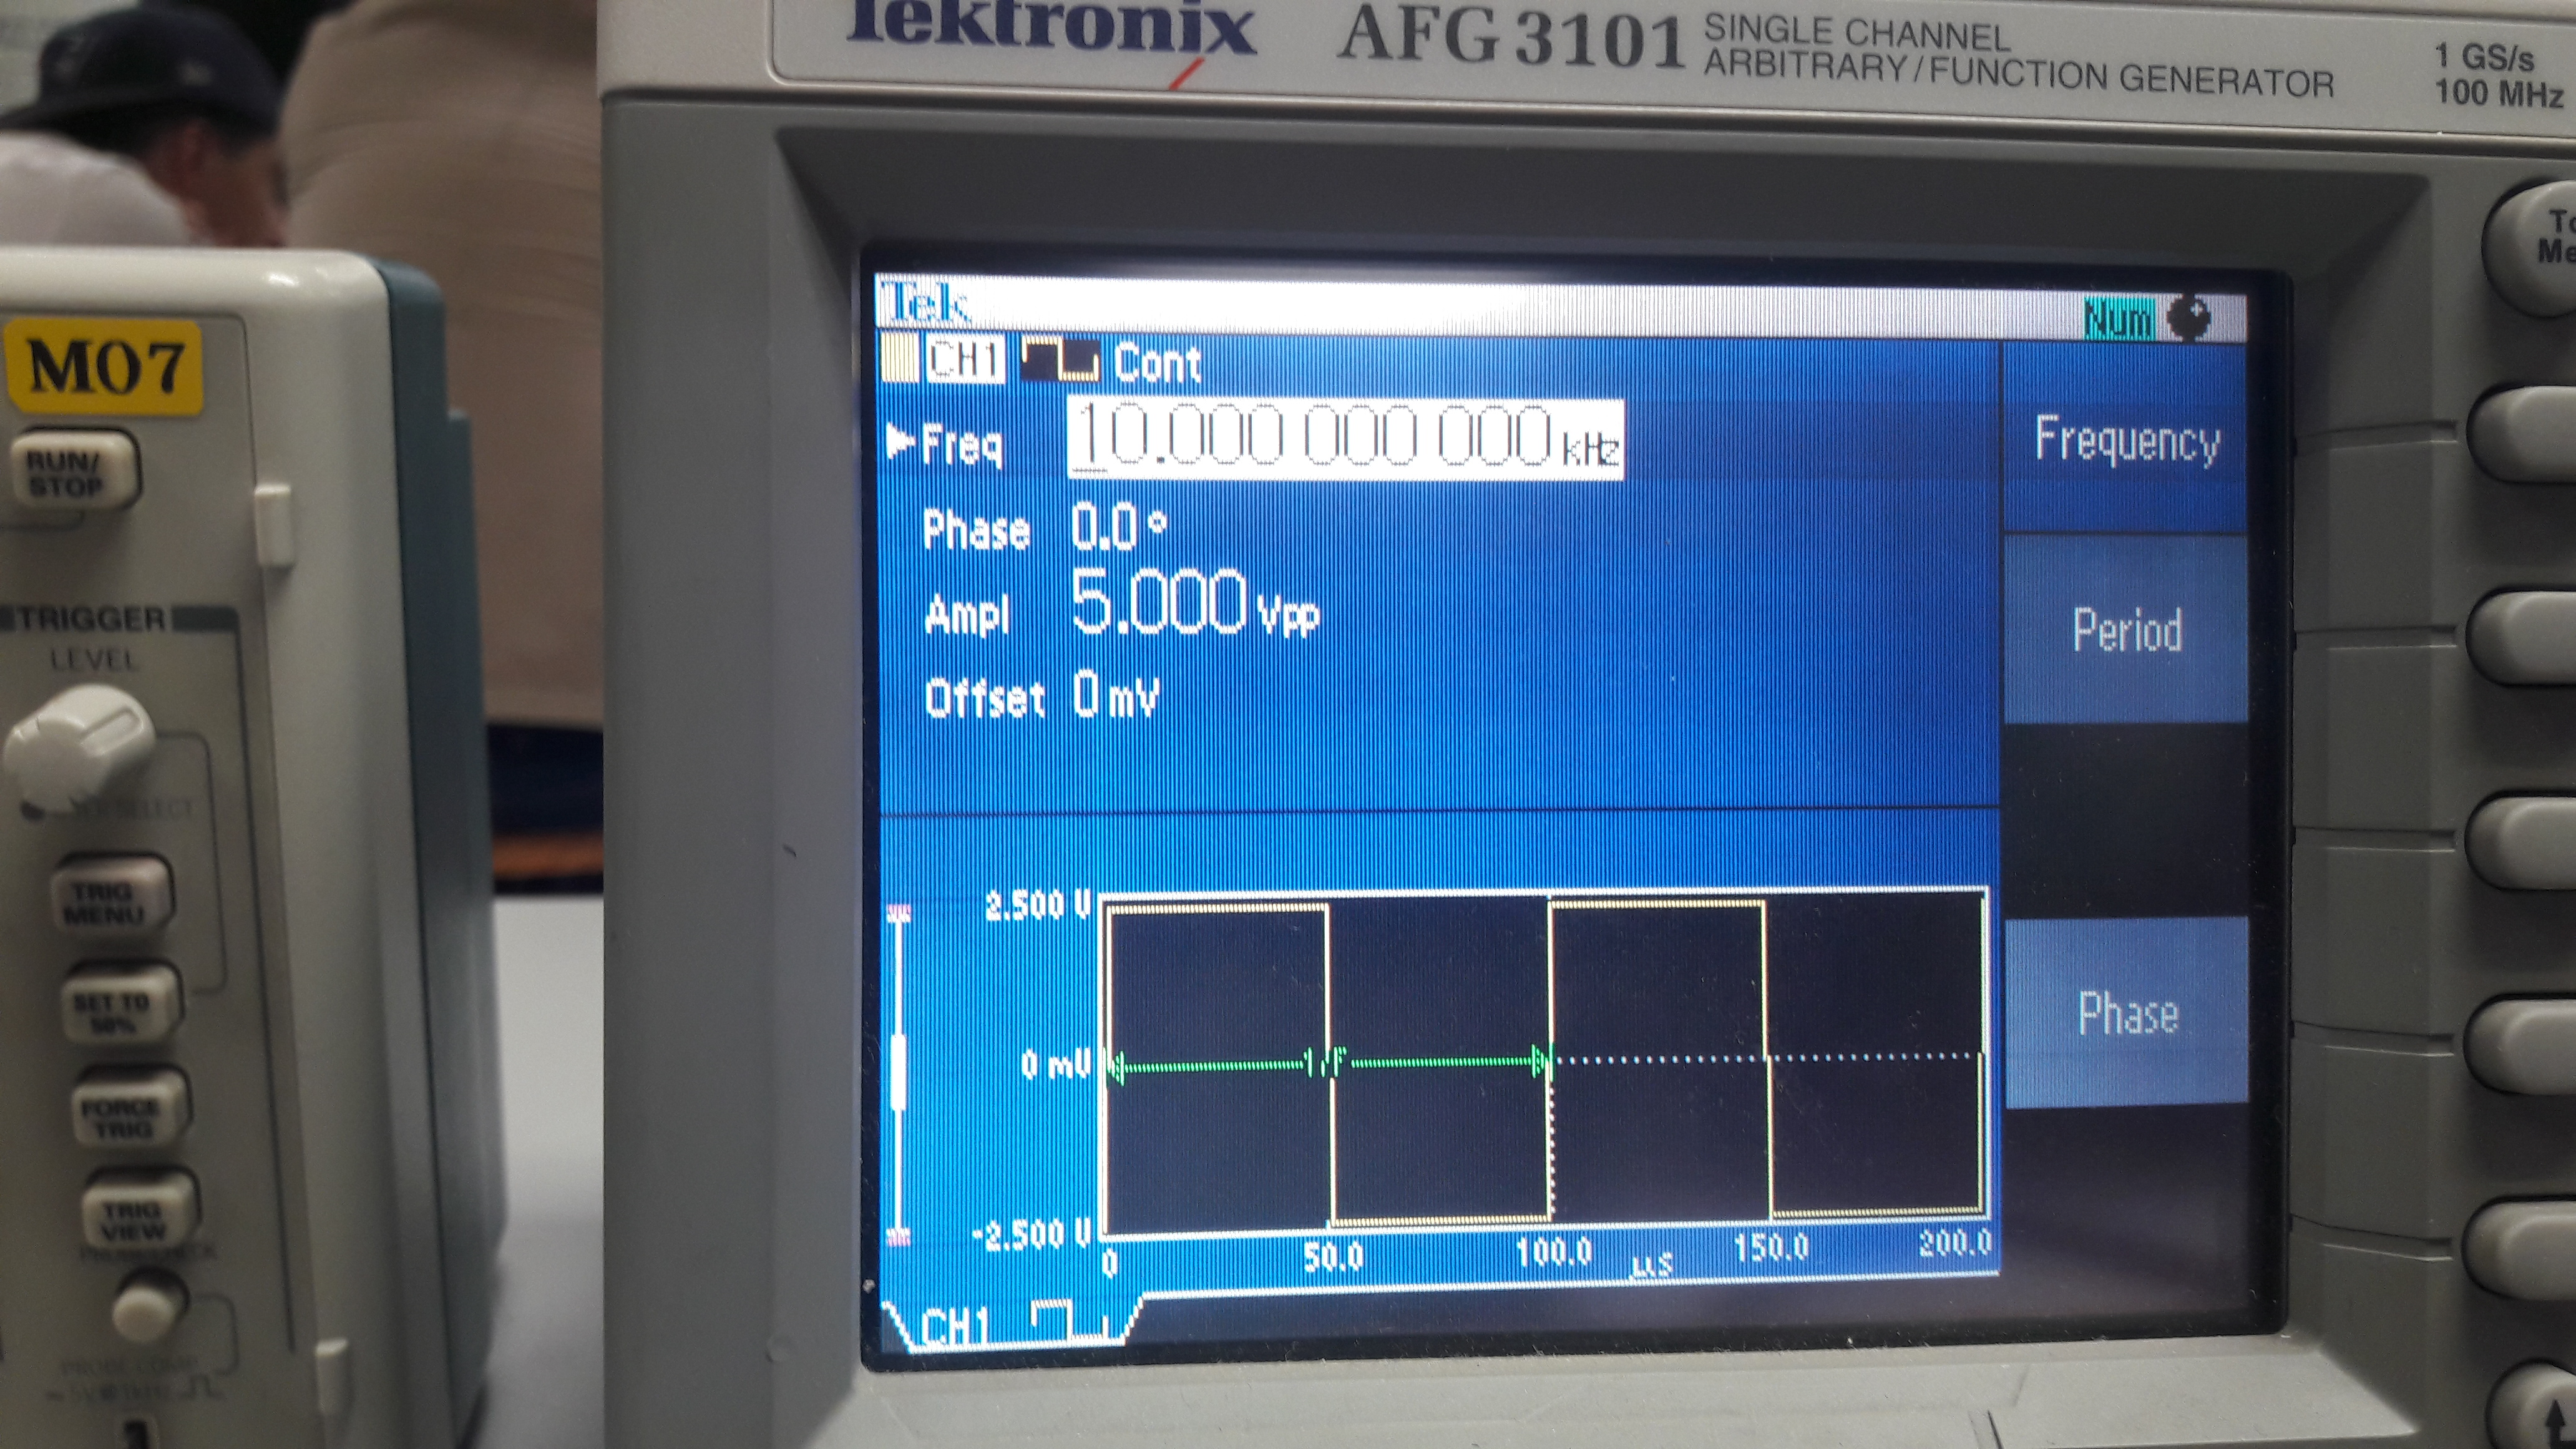
\includegraphics[width=.95\linewidth]{img/part2/10}
        \caption{Signal generator set to produce the square wave}
    \end{subfigure}
    \caption{Square wave generation and display}
\end{figure}
Once with the triangular wave, we set the offset of the signal generator to the maximum, which
was $5 V$, changing the offset moved the signal above in relation to the center of the display, then, when
we set the offset in the negative maximum, the signal moved below the center of the display.\newpage
%Poner foto y valores de máximo y mínimo offset
{\textbf{Minimum Offset}}
\begin{gather*}
    Offset_{MAX} = \SI{5}{\volt}
\end{gather*}
\begin{figure}[H]
    \begin{subfigure}{0.55\textwidth}
        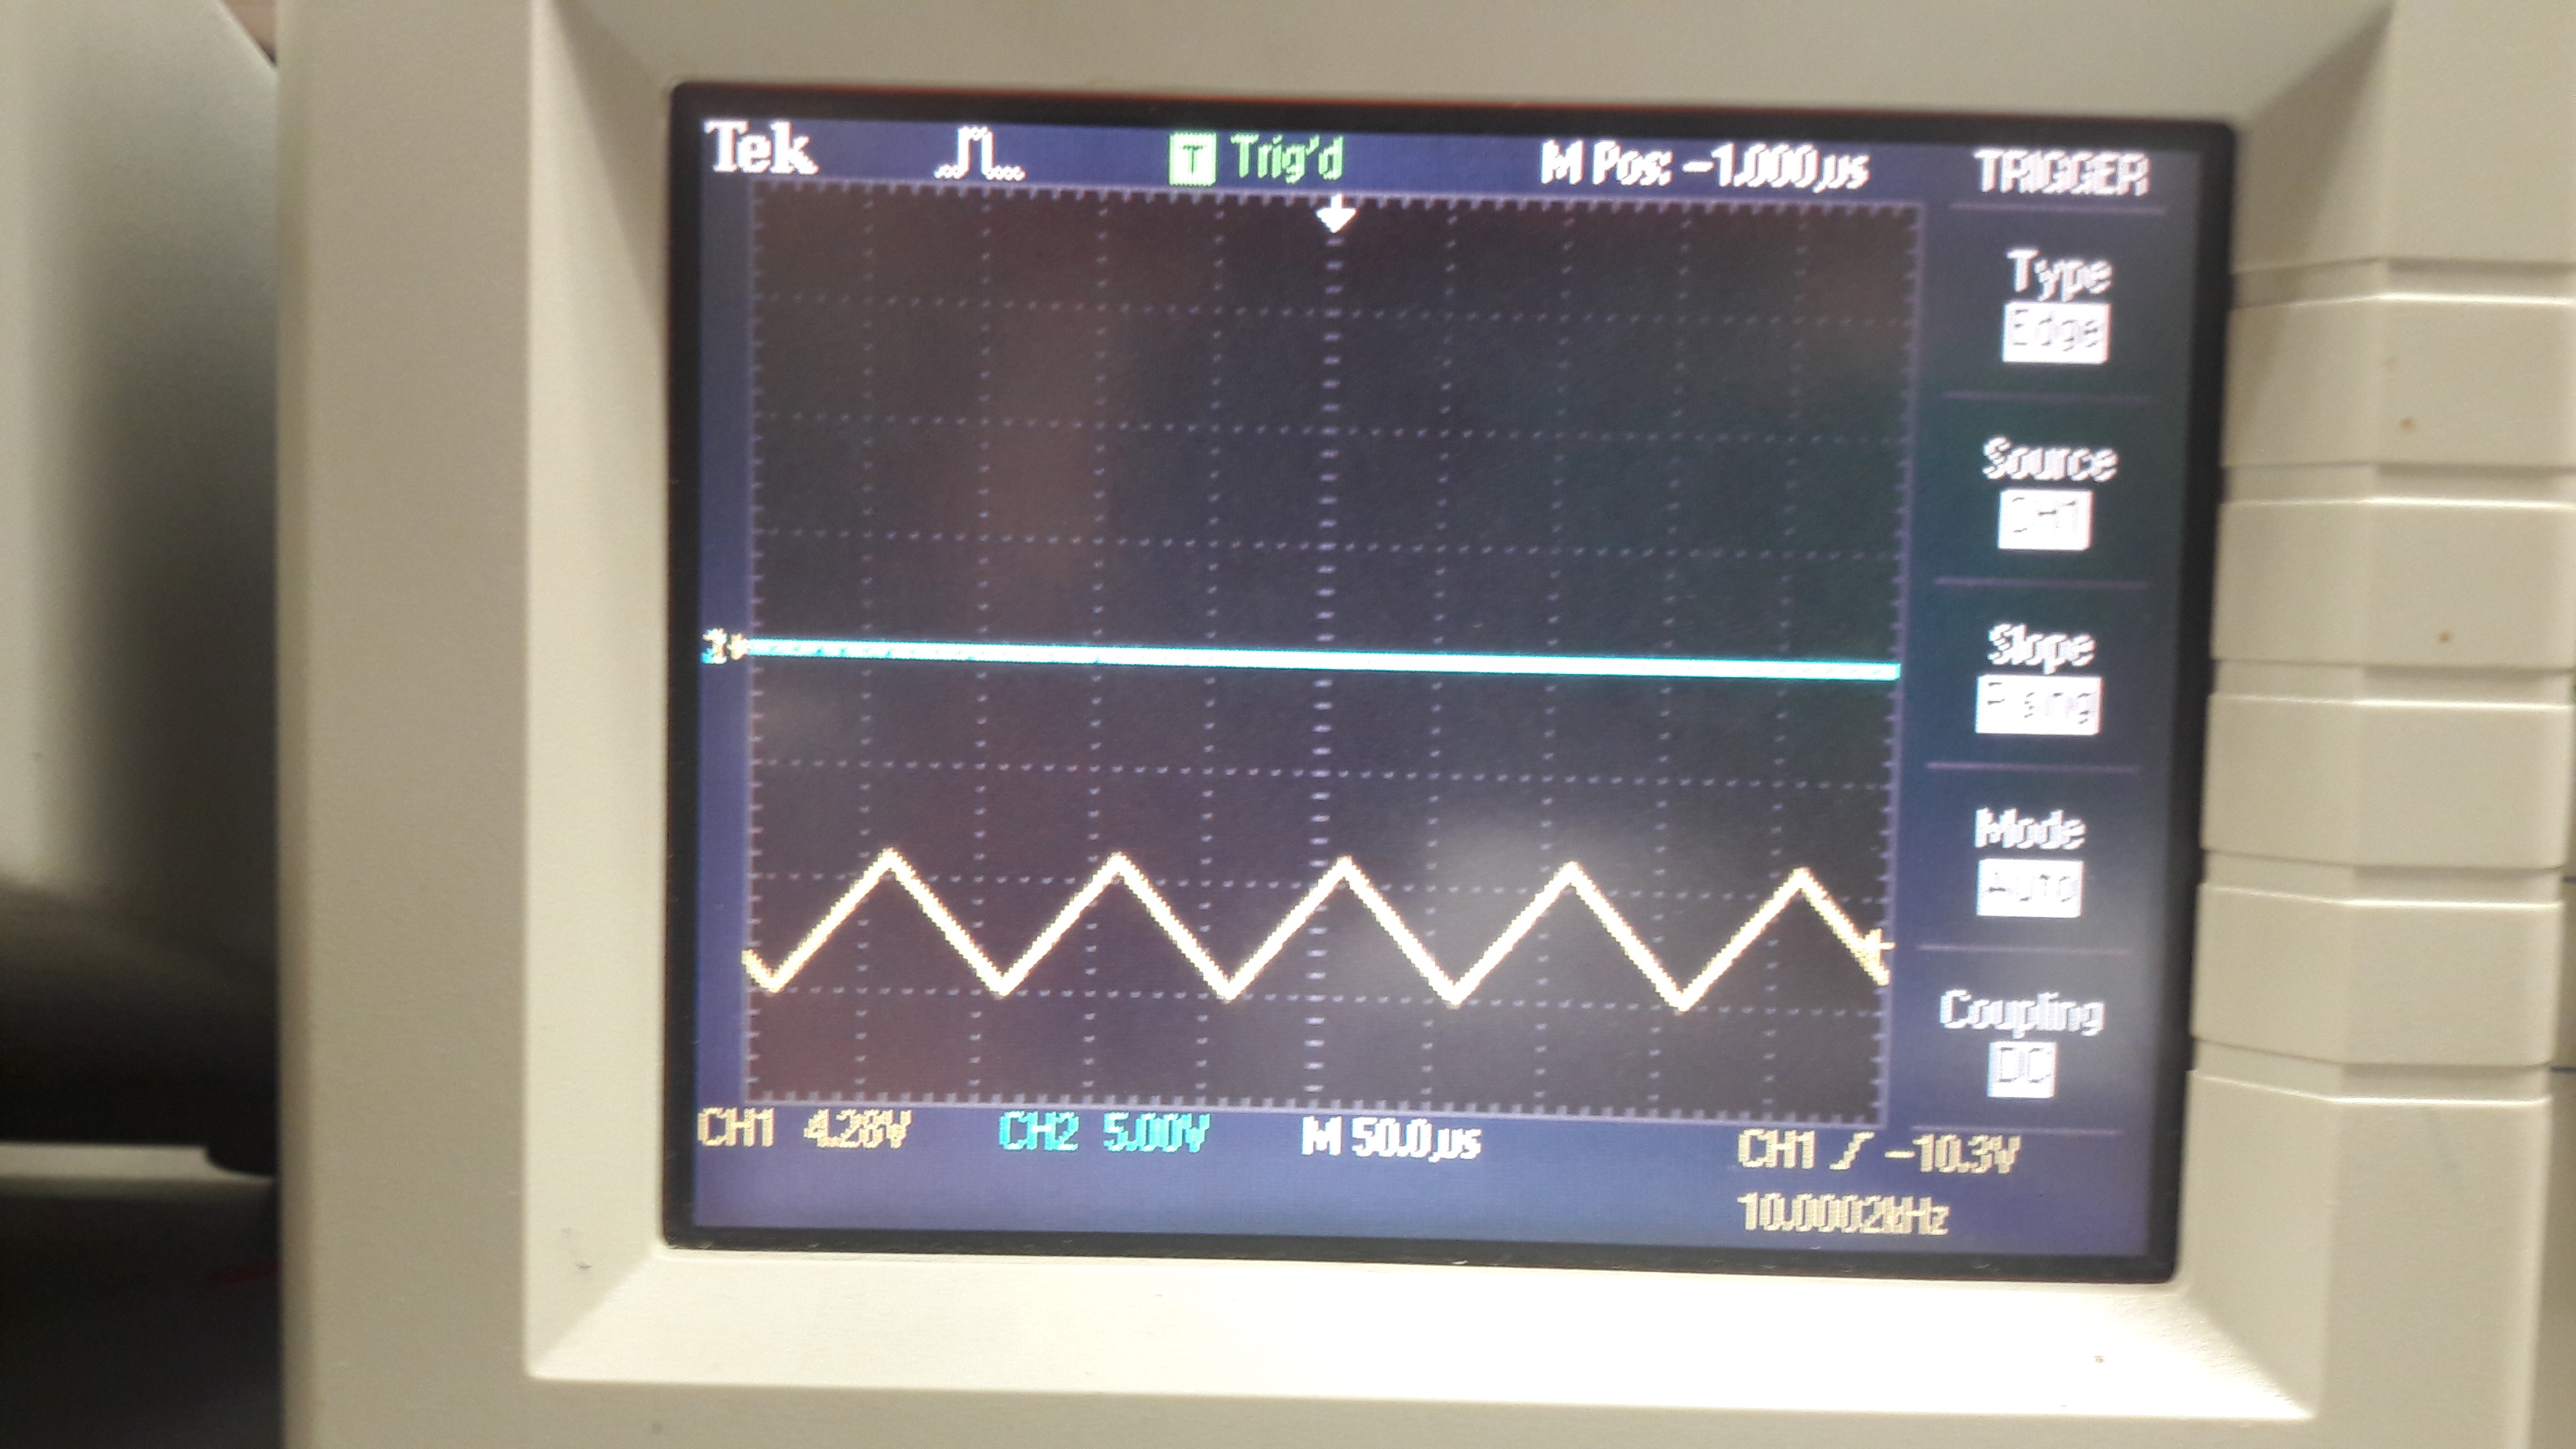
\includegraphics[width=.95\linewidth]{img/part2/15}
    \end{subfigure}
    \begin{subfigure}{0.55\textwidth}
        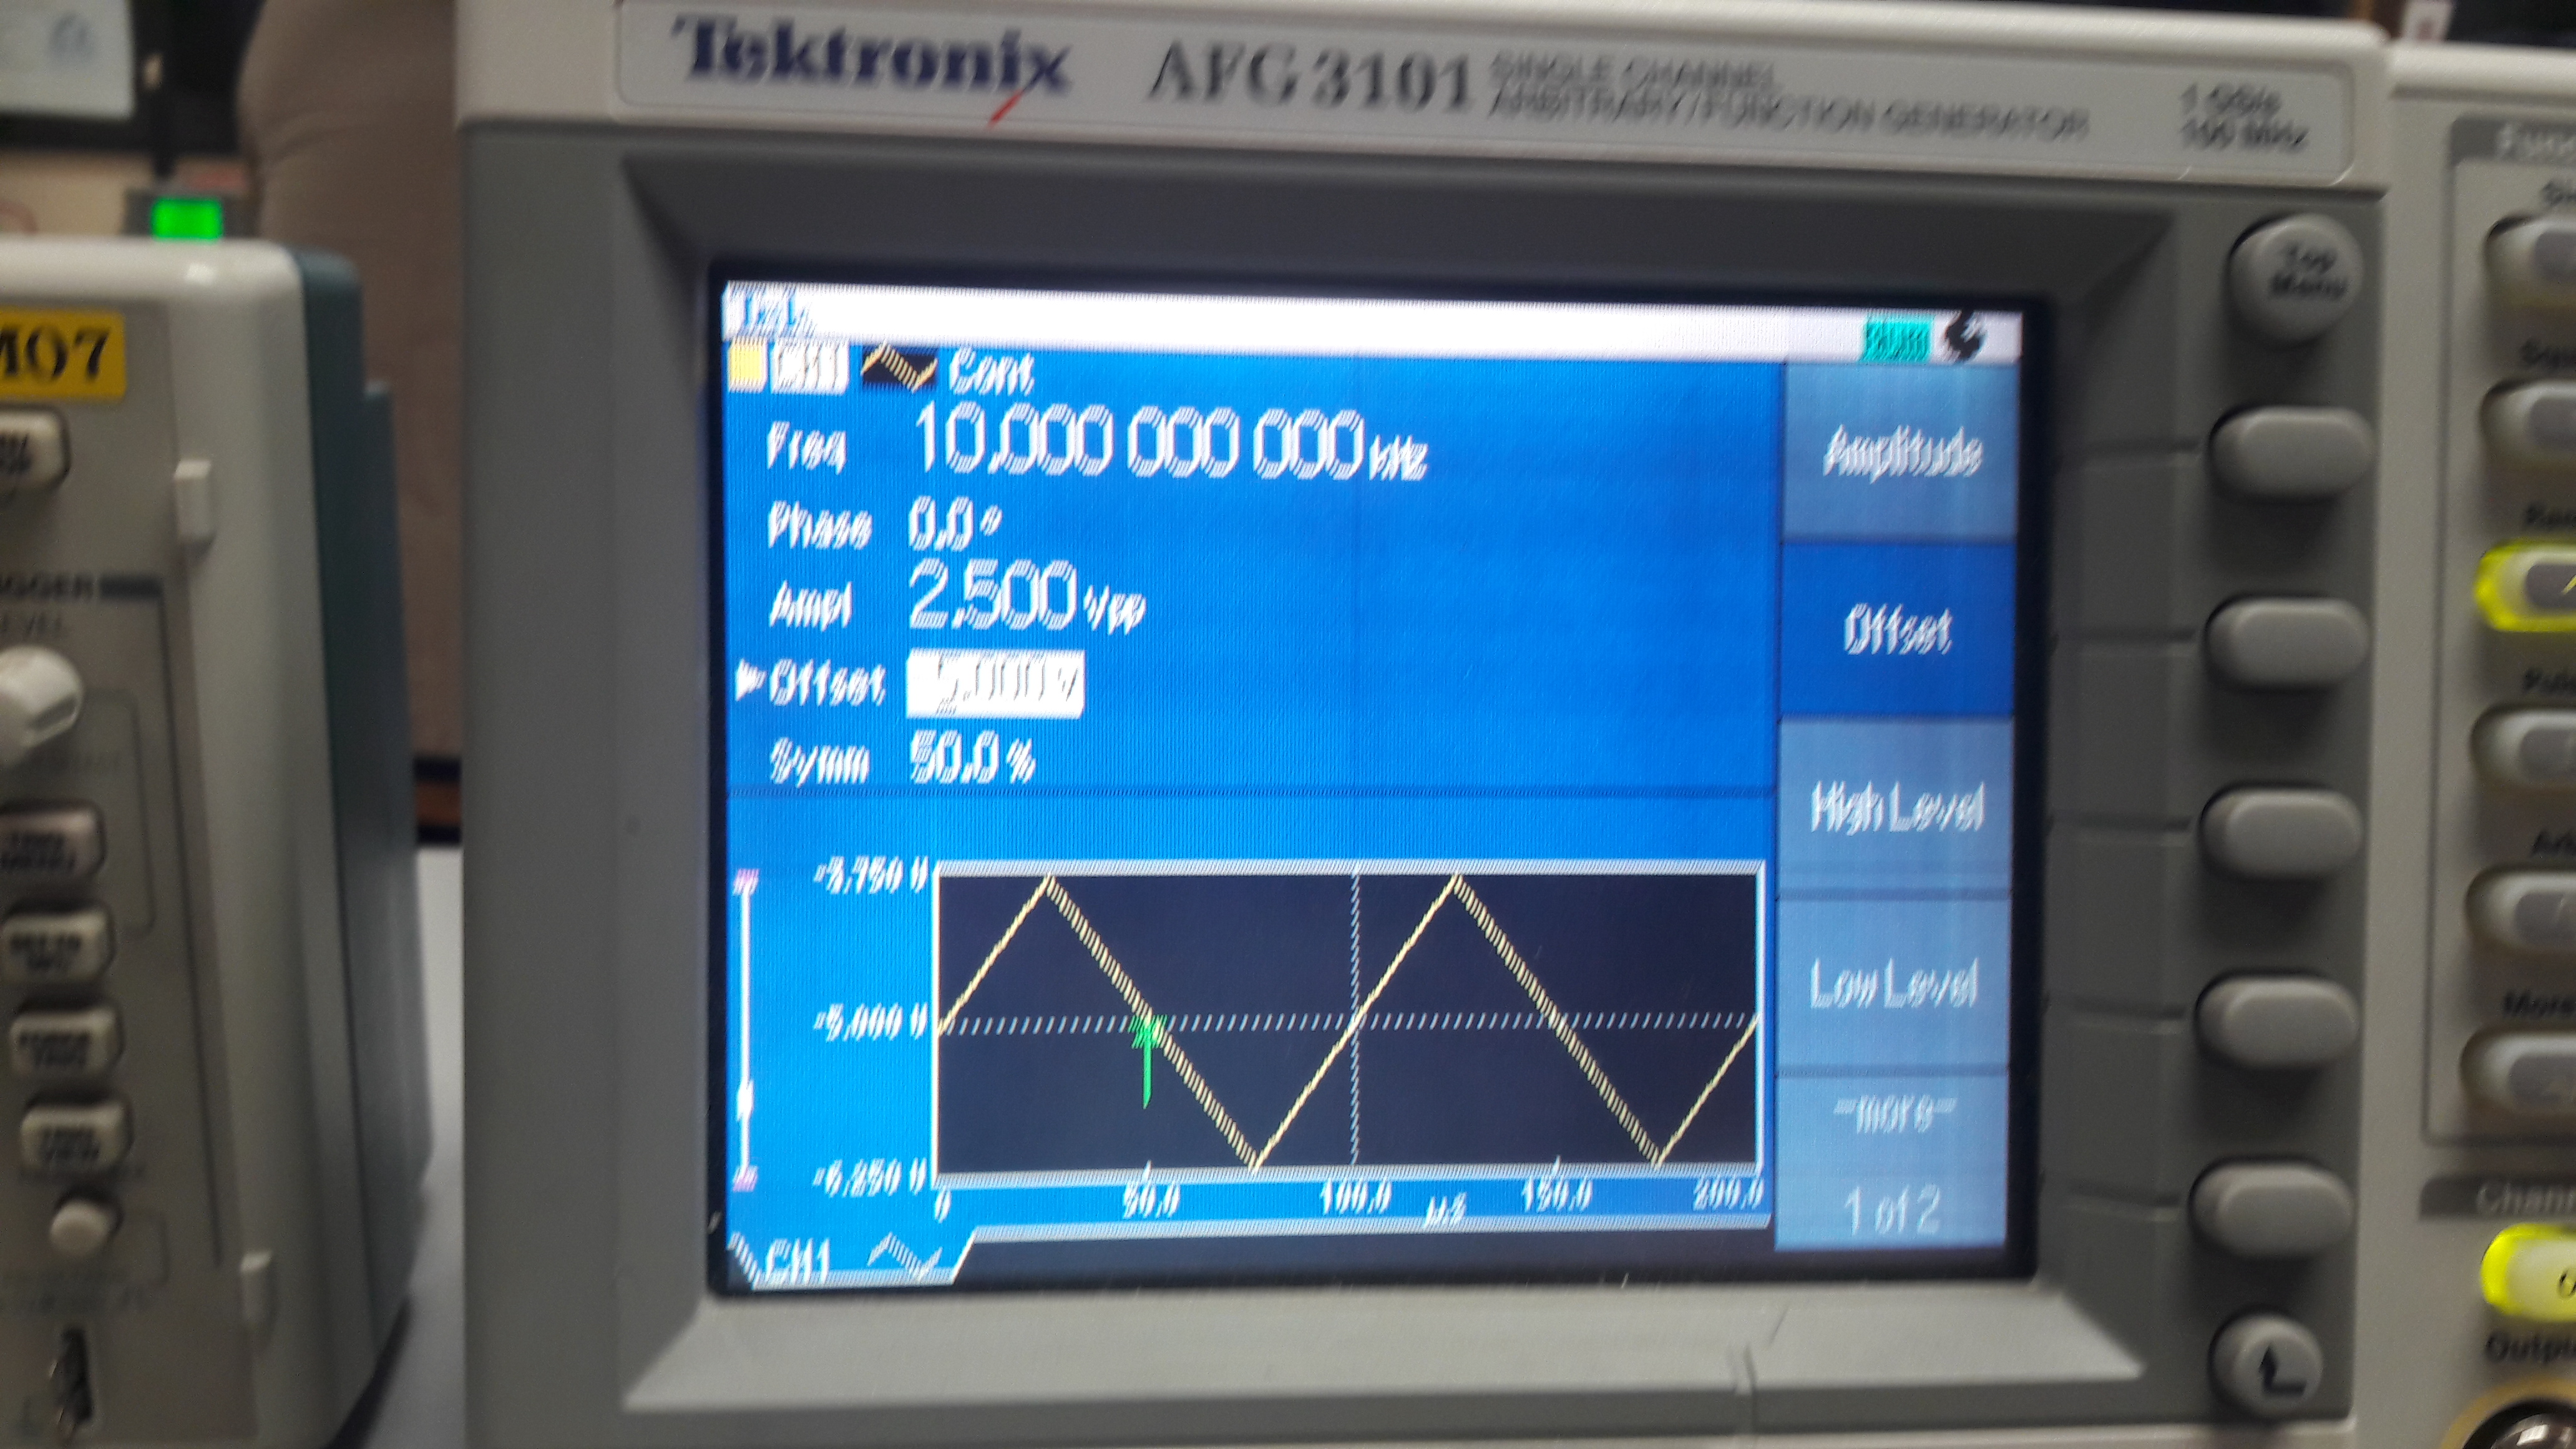
\includegraphics[width=.95\linewidth]{img/part2/14}
    \end{subfigure}
    \caption{Minimum offset available in the signal generator}
\end{figure}
{\textbf{Maximum Offset}}
\begin{gather*}
    Offset_{MAX} = \SI{5}{\volt}
\end{gather*}
\begin{figure}[H]
    \begin{subfigure}{0.55\textwidth}
        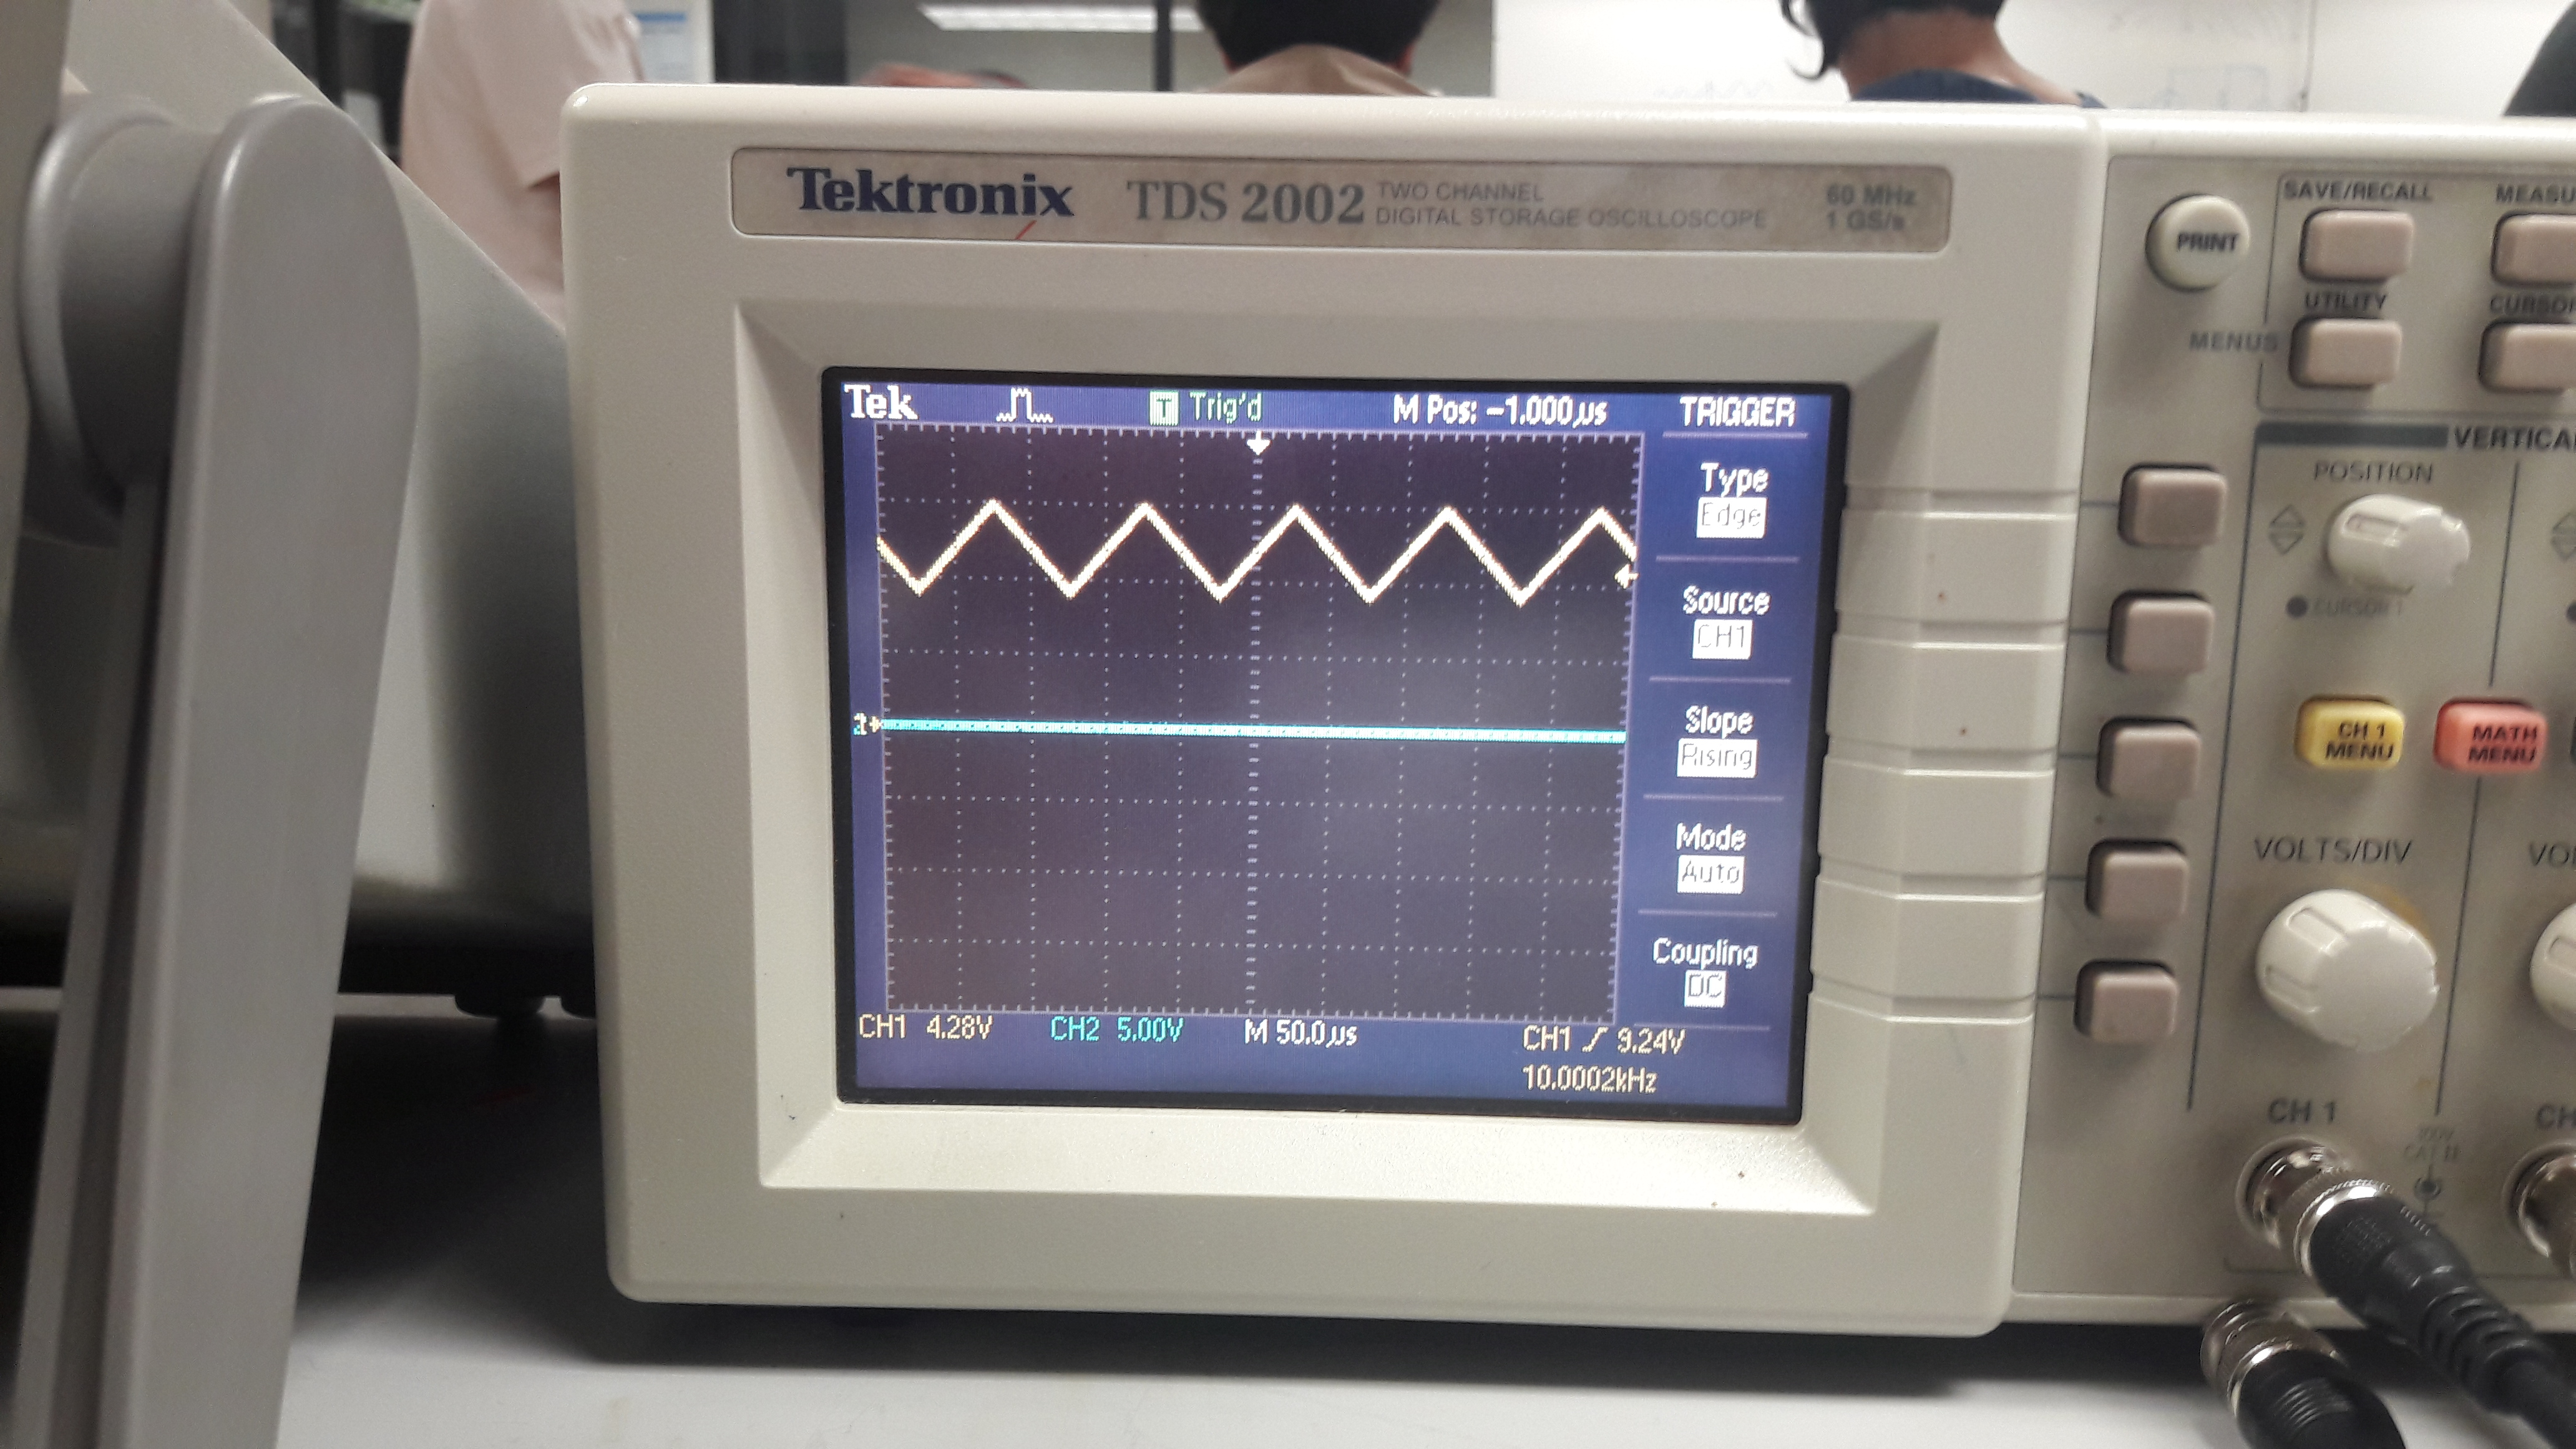
\includegraphics[width=.95\linewidth]{img/part2/13}
    \end{subfigure}
    \begin{subfigure}{0.55\textwidth}
        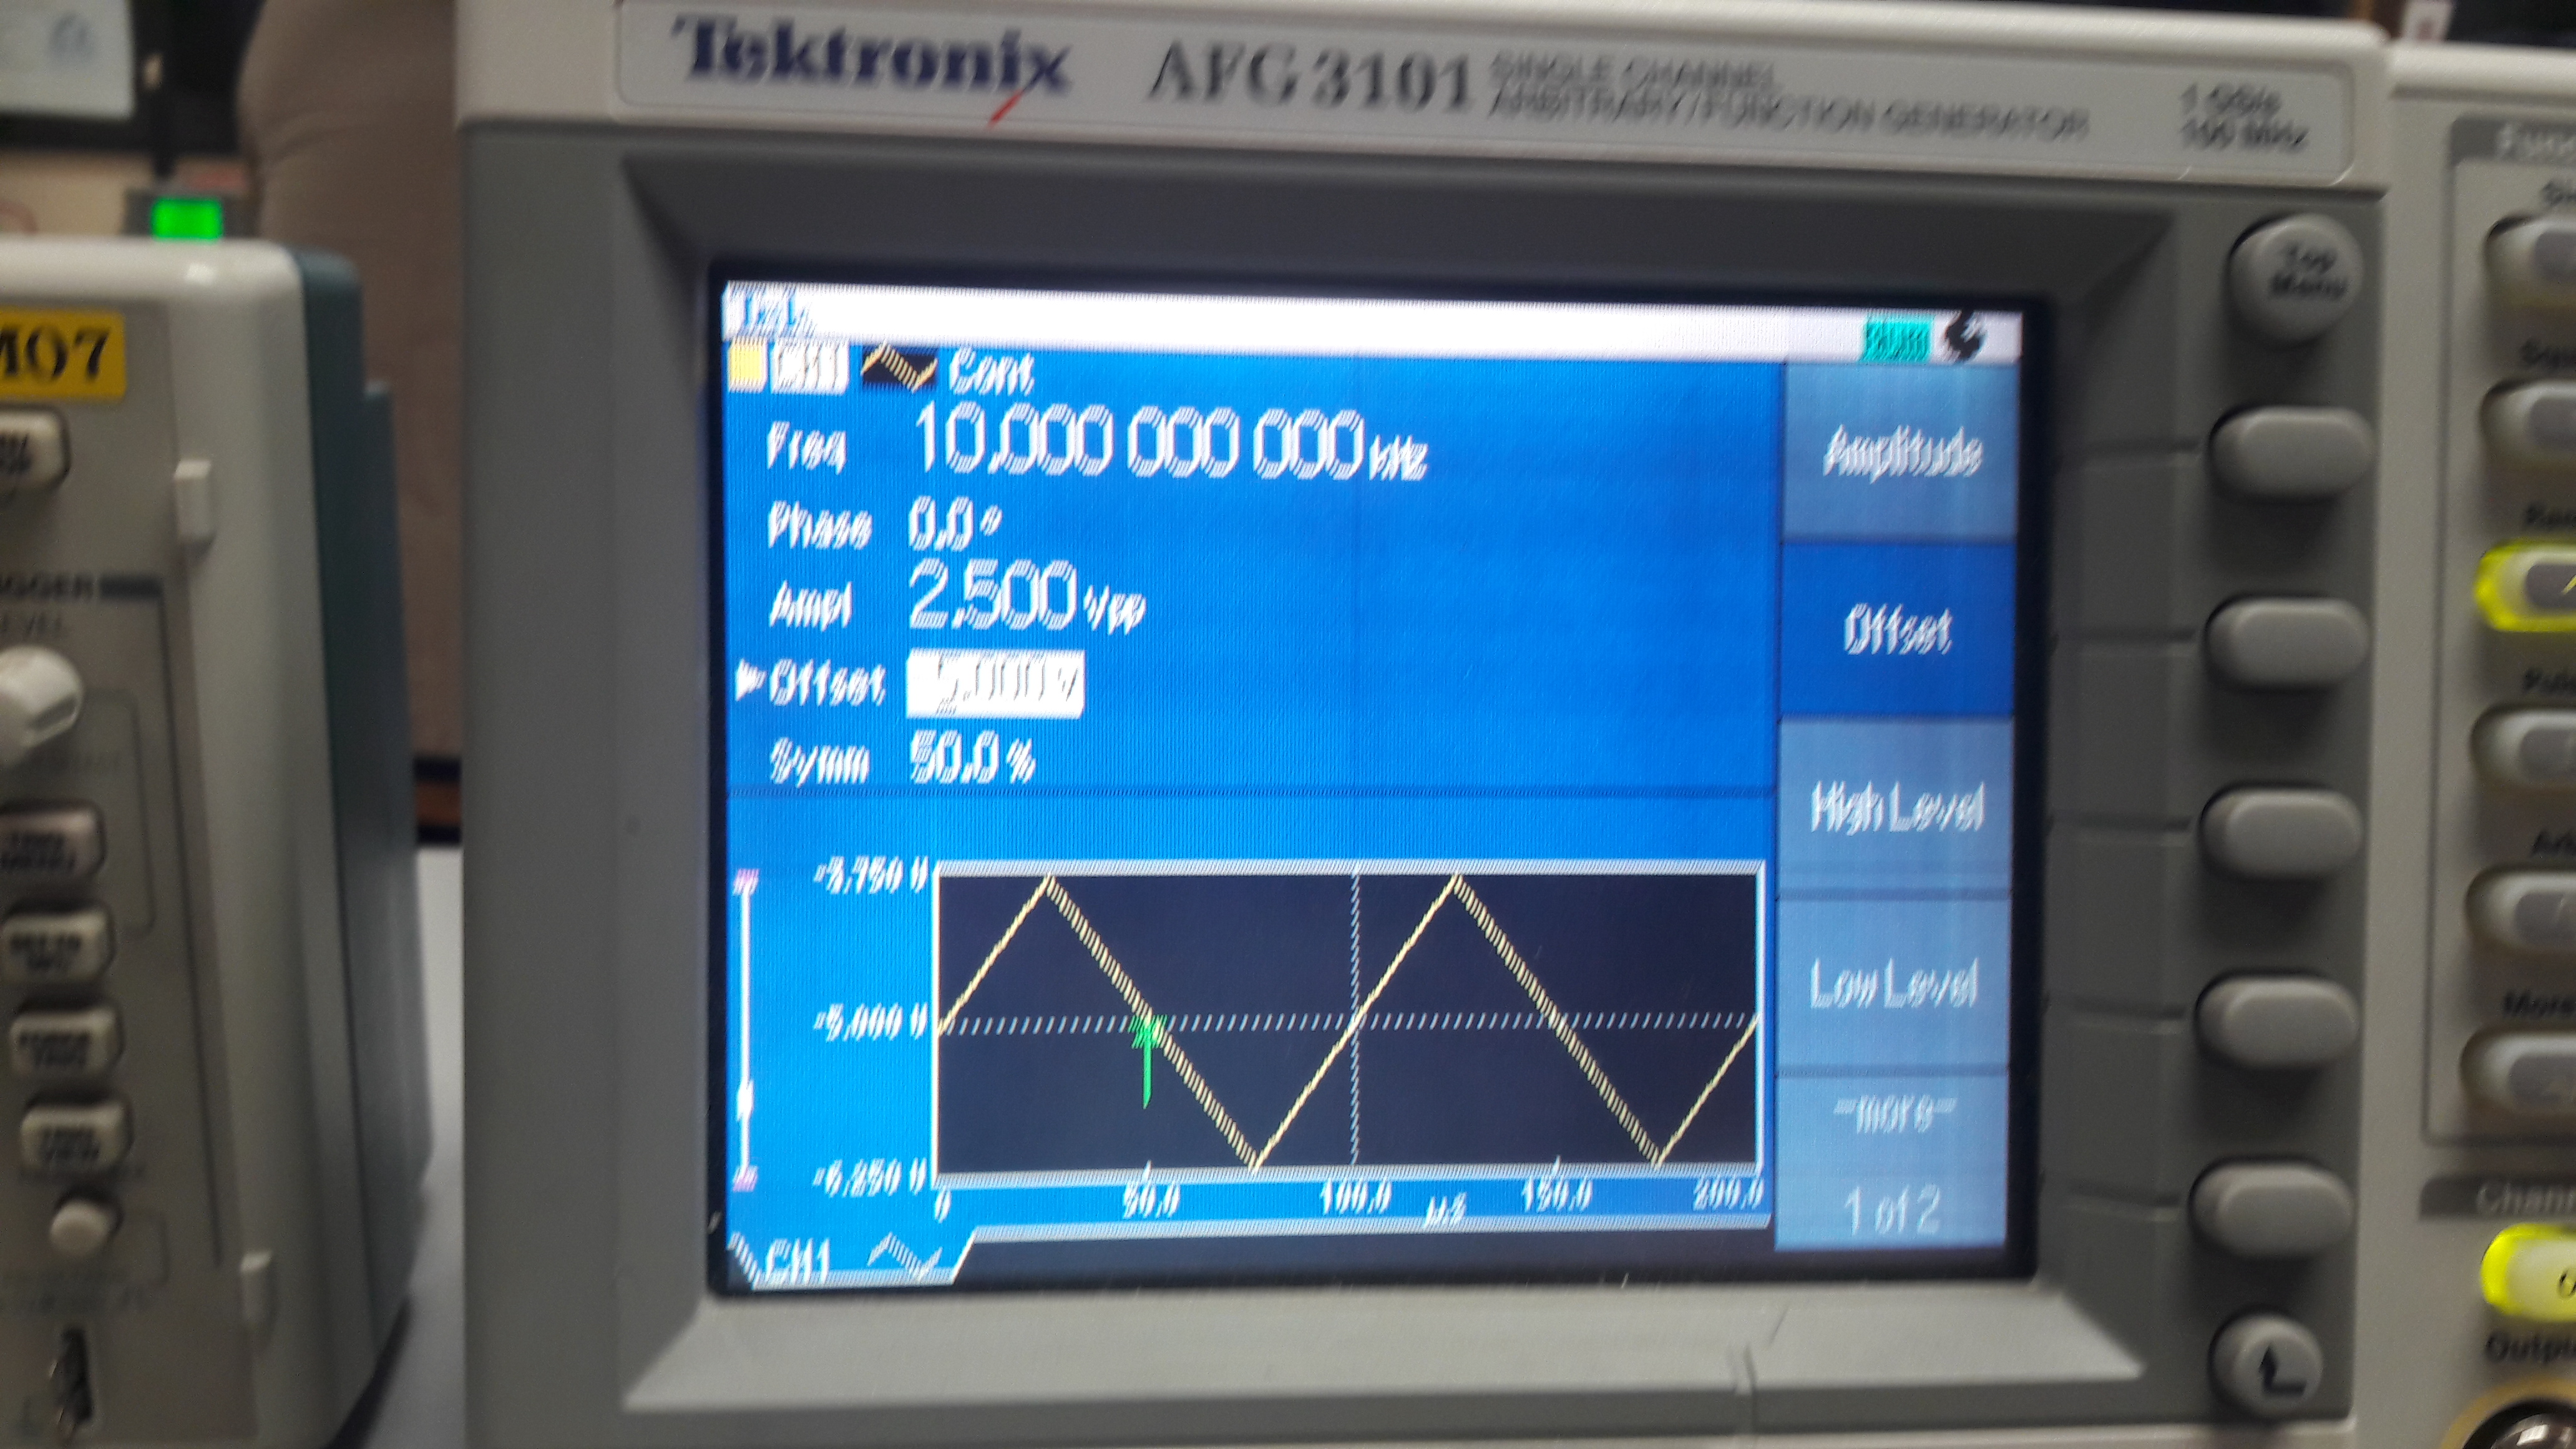
\includegraphics[width=.95\linewidth]{img/part2/14}
    \end{subfigure}
    \caption{Maximum offset available in the signal generator}
\end{figure}
\subsection{The oscilloscope as an X-Y plotter with DC currents}
Using the circuit shown in the diagram:
\begin{figure}[H]
    \centering
    \begin{circuitikz}
        \draw (0,0) -- (4,0) to [short,-*](6,0)
        (0,3) to [sV = $12 V_{pp}\,\SI{300}{\hertz}$](0,0)
        (0,3) to [C = \SI{0.1}{\micro\farad},*-*] (6,3)
        (4,3) to [R=$\SI{4.7}{\kilo\ohm}$,*-*](4,0)
        (0,3) -- (0,4) to [short,-*](6,4)
        {
            [anchor = south west](6,0) node {T}
            [anchor = south west](6,3) node {Y}
            [anchor = south west](6,4) node {X}
        };
    \end{circuitikz}
\end{figure}
We changed the mode of the oscilloscope yo X-Y, then, with each channel in ground coupling, we set
the trace for each channel to match the point at the center of the display. 
\begin{figure}[H]
    \centering
    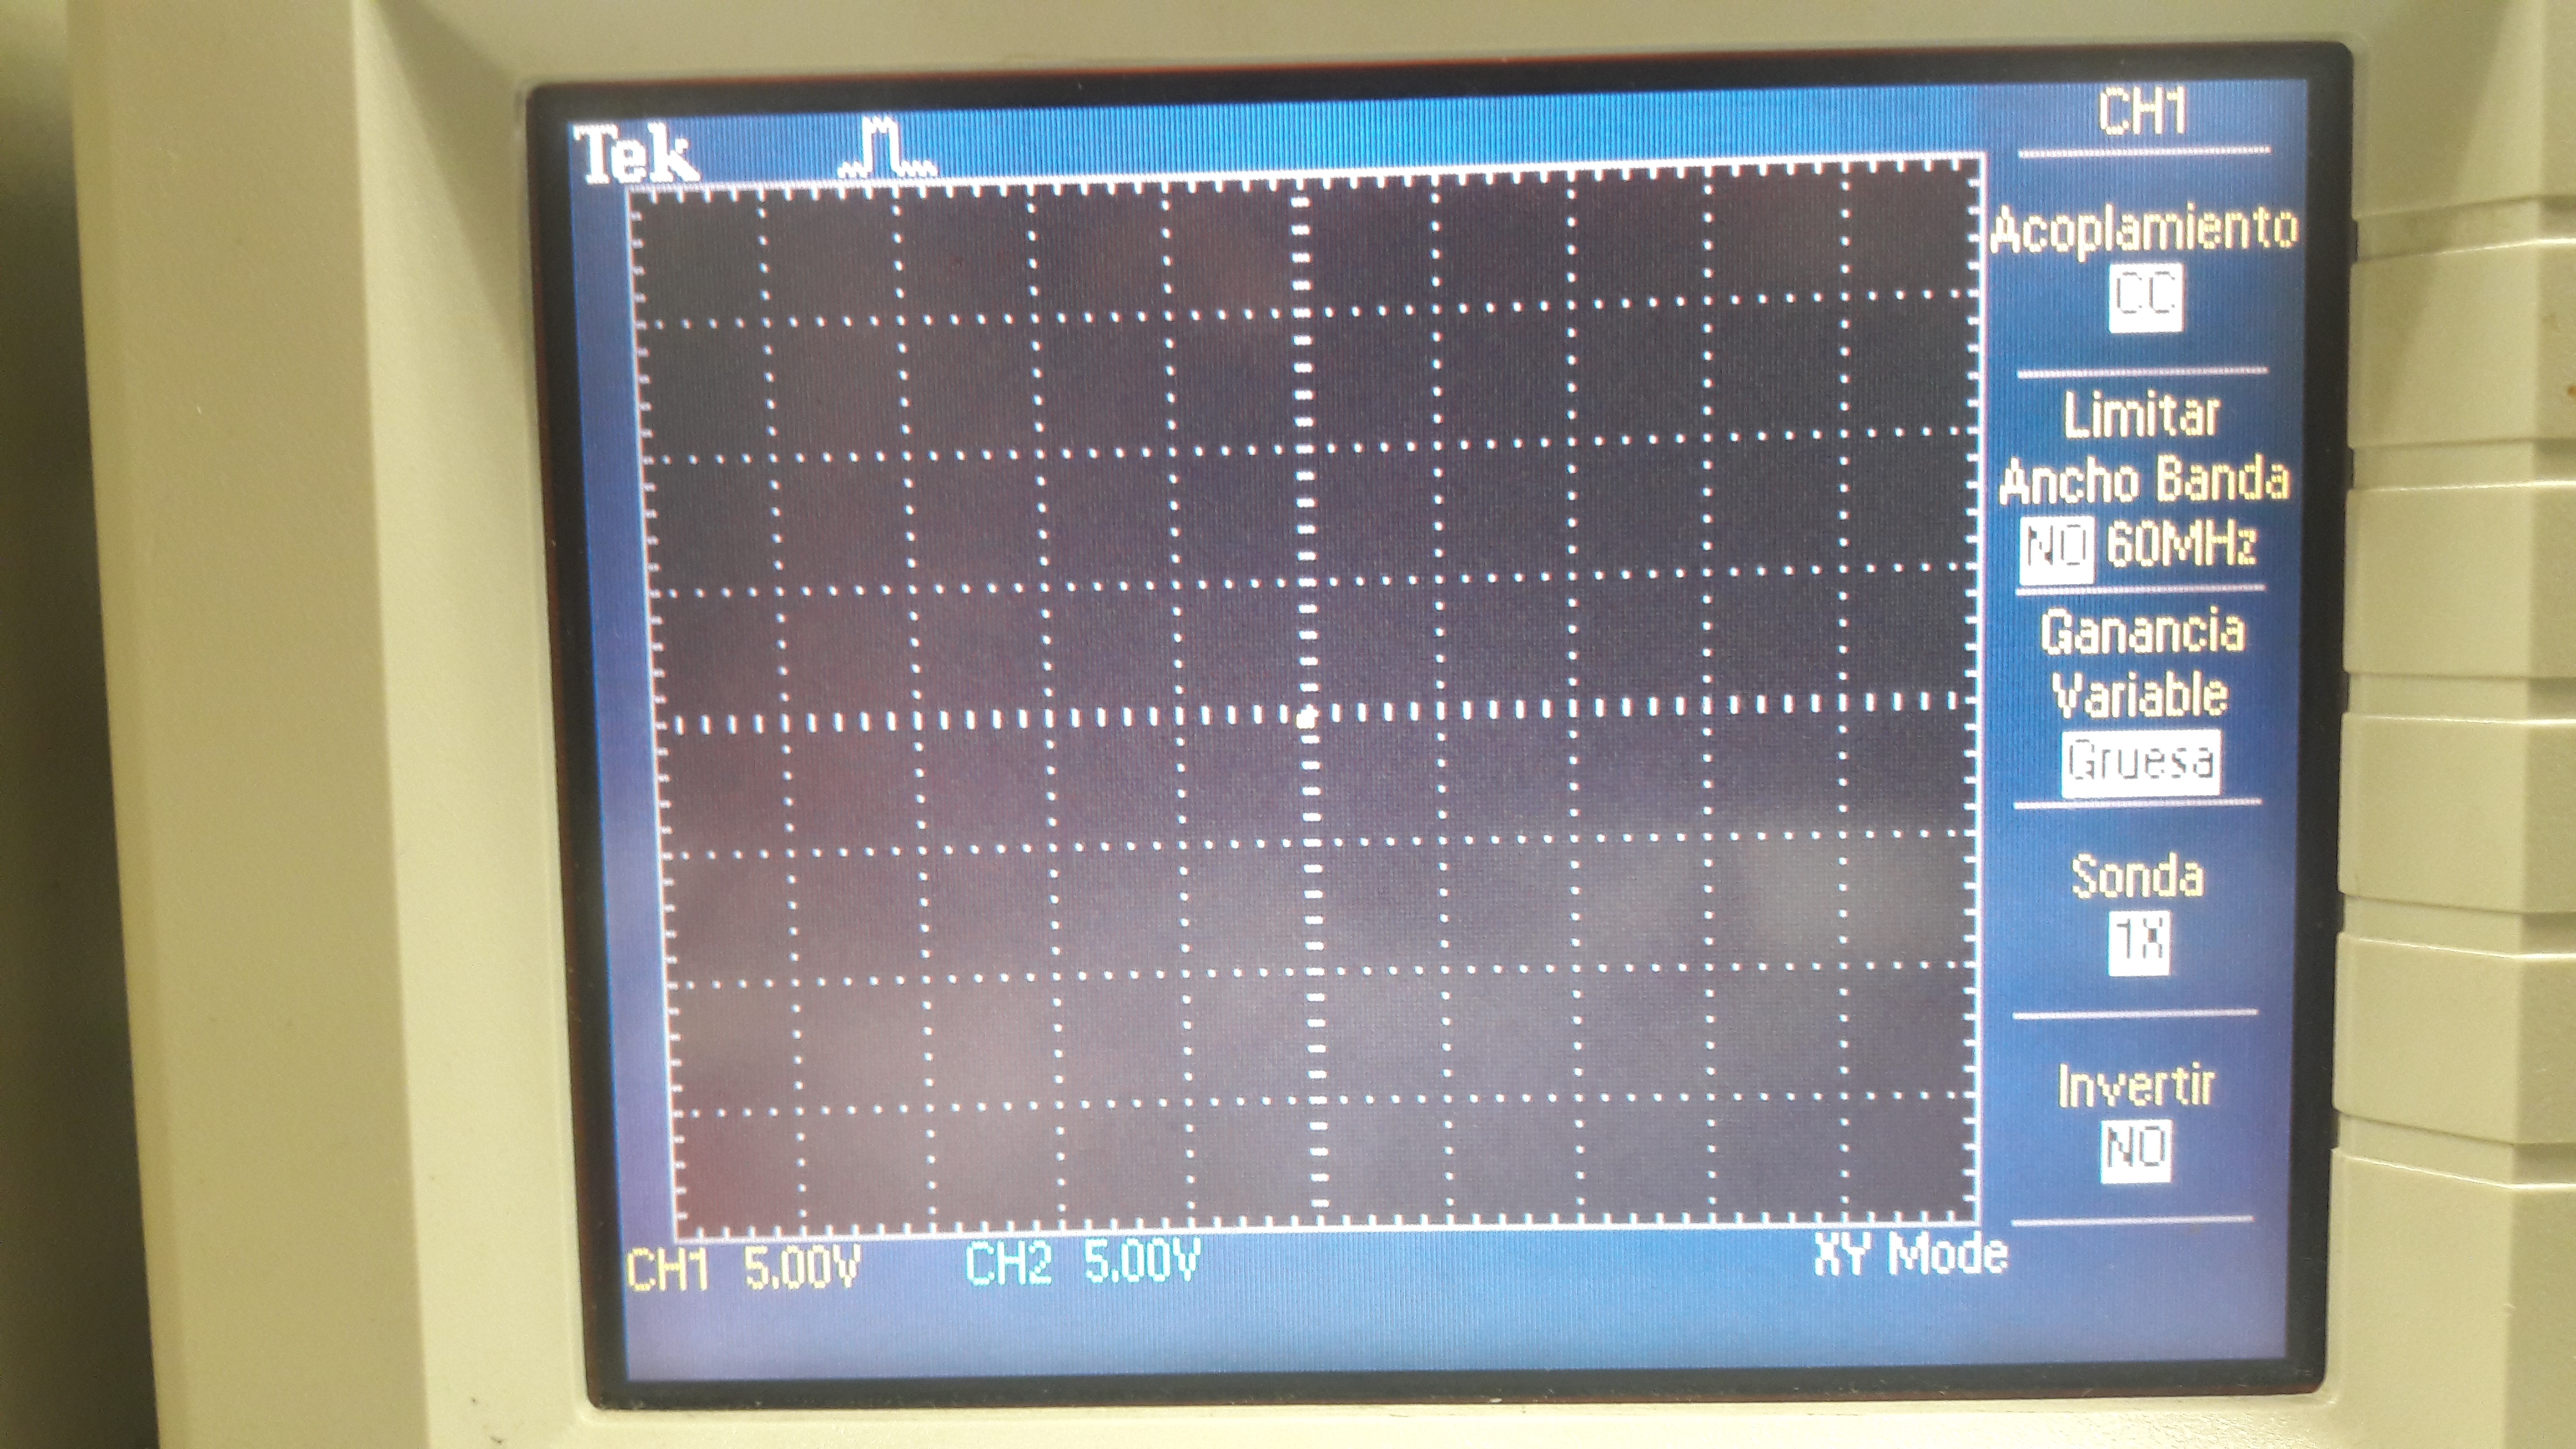
\includegraphics[width=.5\linewidth]{img/part3/6}
    \caption{Oscilloscope with both X and Y channels in ground coupling matching the center of the
    grid}
\end{figure}
\subsubsection{Measurements}
Later, we clipped the test probes to certain points of the circuit as follows:
\begin{enumerate}
    \item Positive of channel X to point A and negative of channel X to point C
    \item Positive of channel Y to point B and negative of channel Y to point C
\end{enumerate}
%Primera foto
\begin{figure}[H]
    \centering
    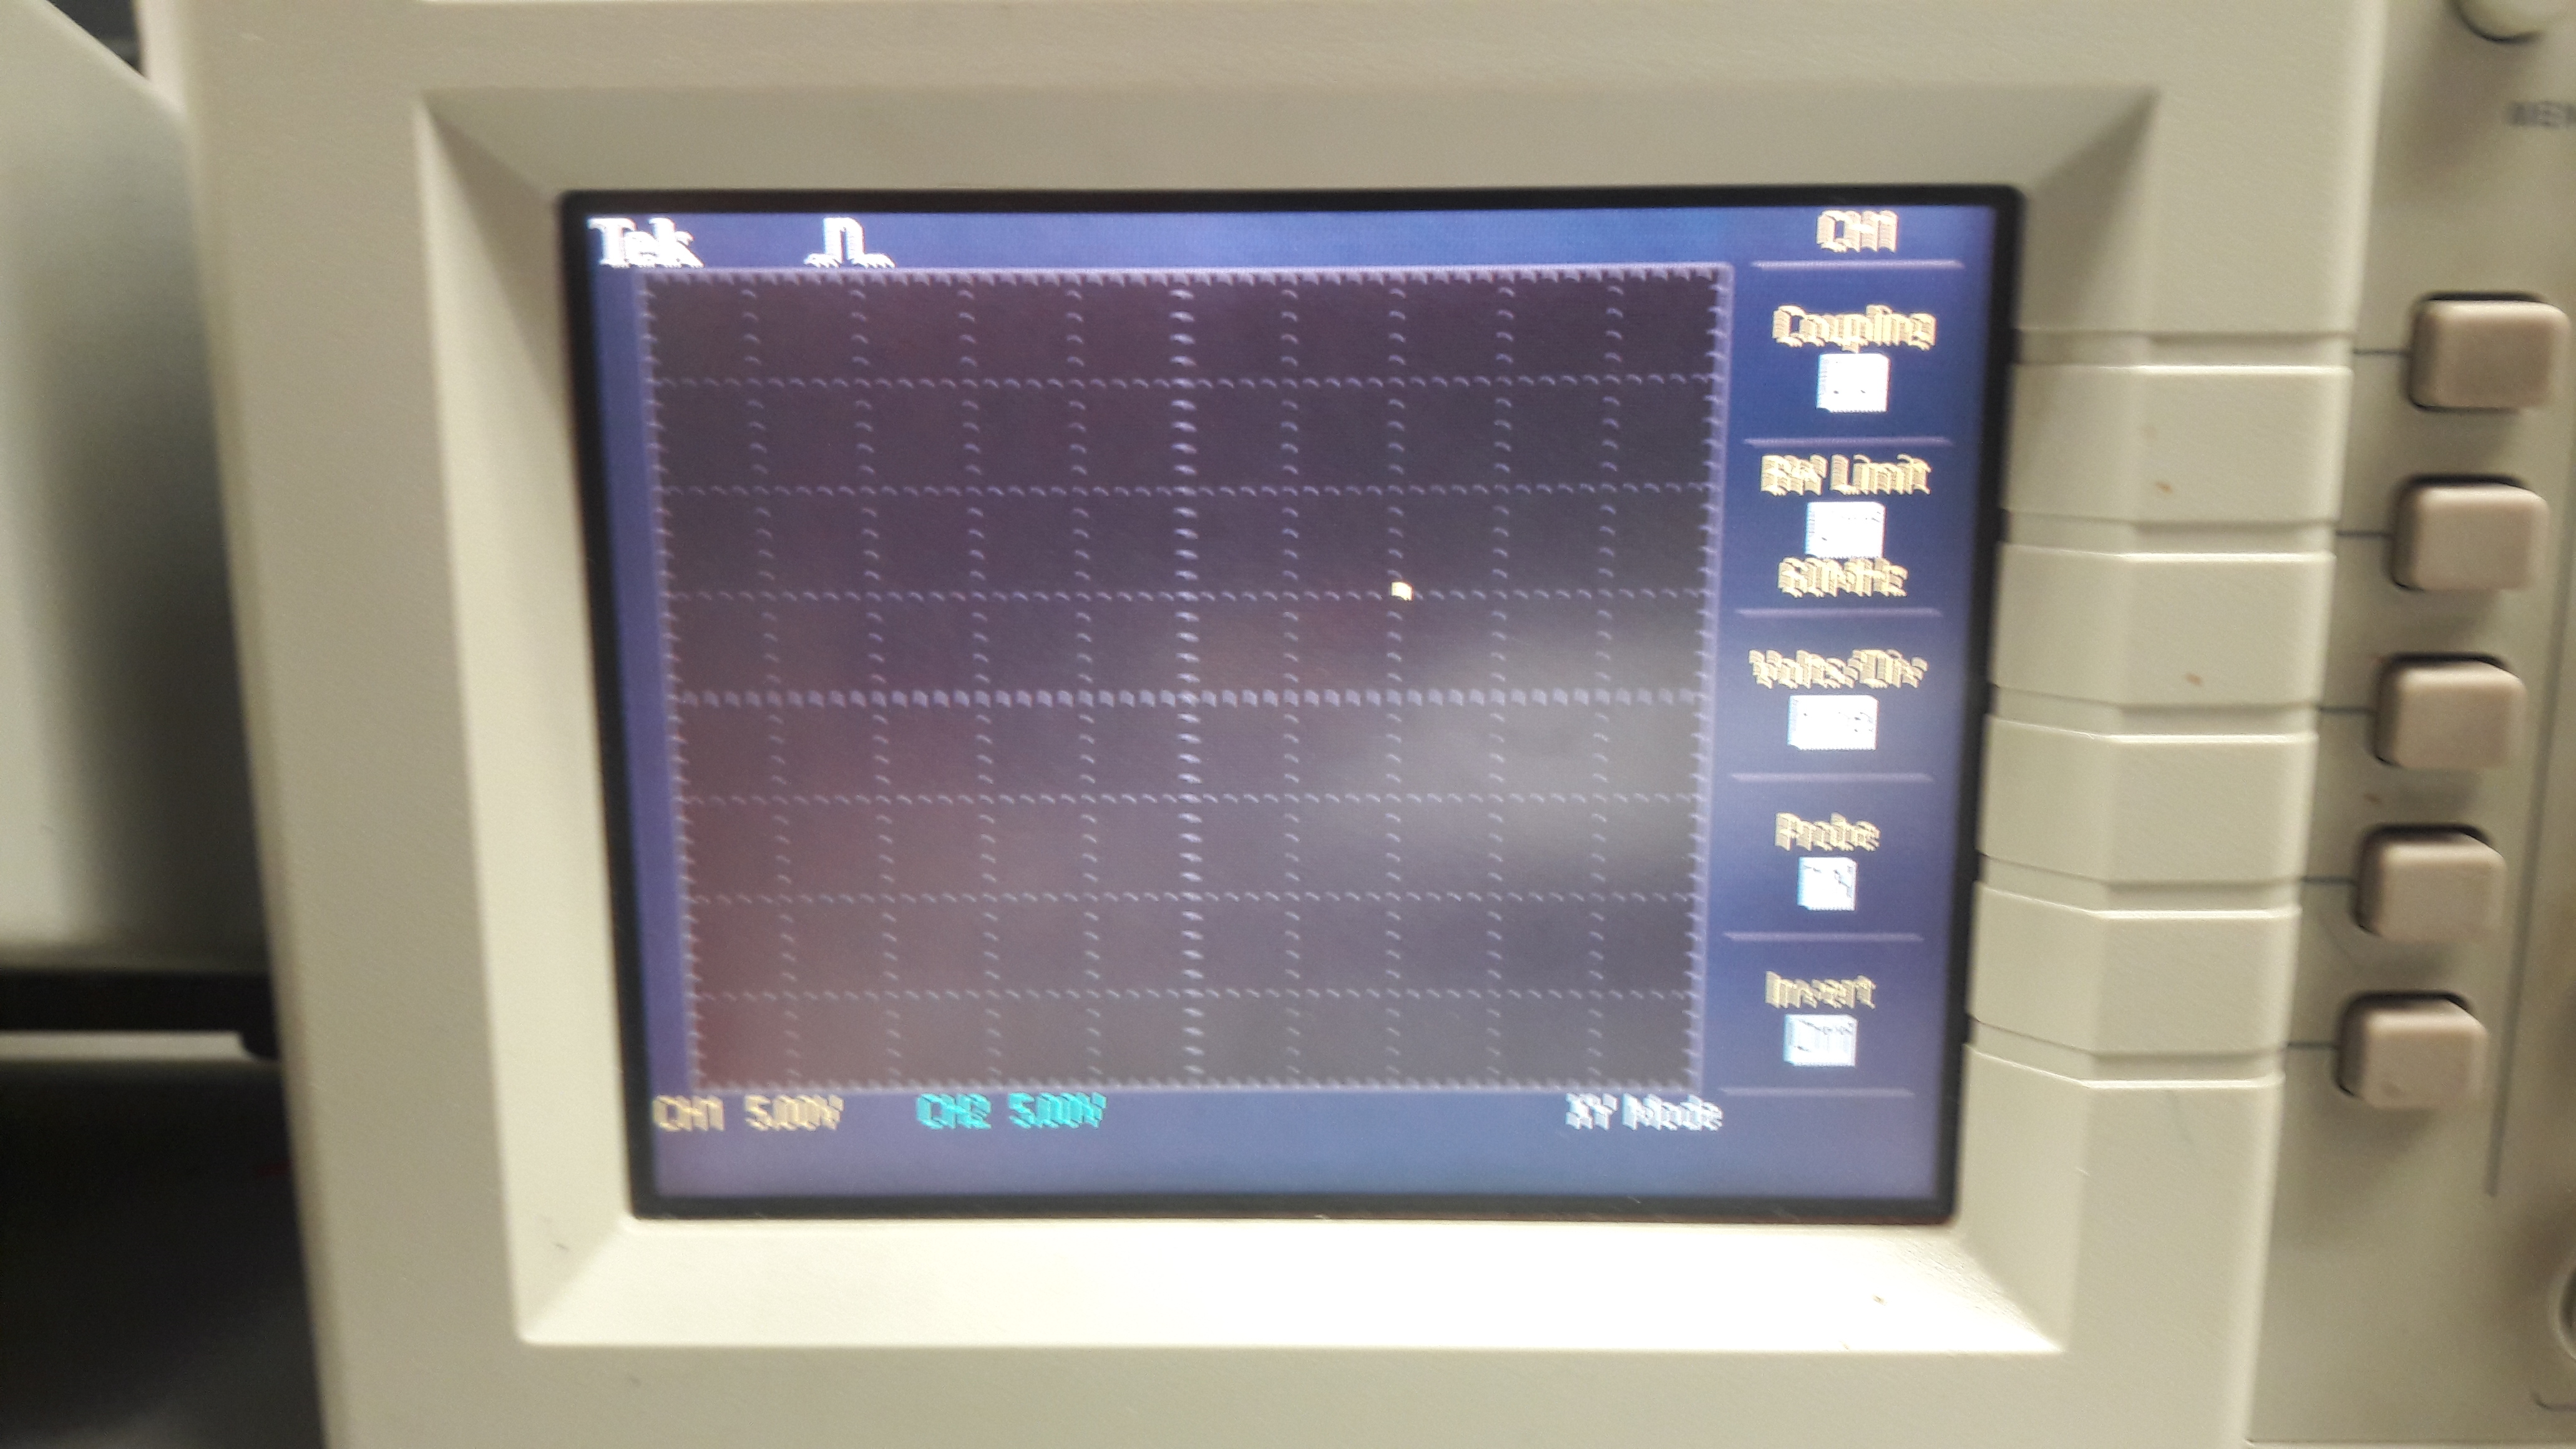
\includegraphics[width=.5\linewidth]{img/part3/2}
    \caption{Oscilloscope with channels connected according to steps 1 and 2}
\end{figure}
\begin{enumerate}
    \setcounter{enumi}{2}
\item Positive of channel X to point A and positive of channel Y to point B, the negatives of both
channels to point C.
\end{enumerate}
%Segunda foto
\begin{figure}[H]
    \centering
    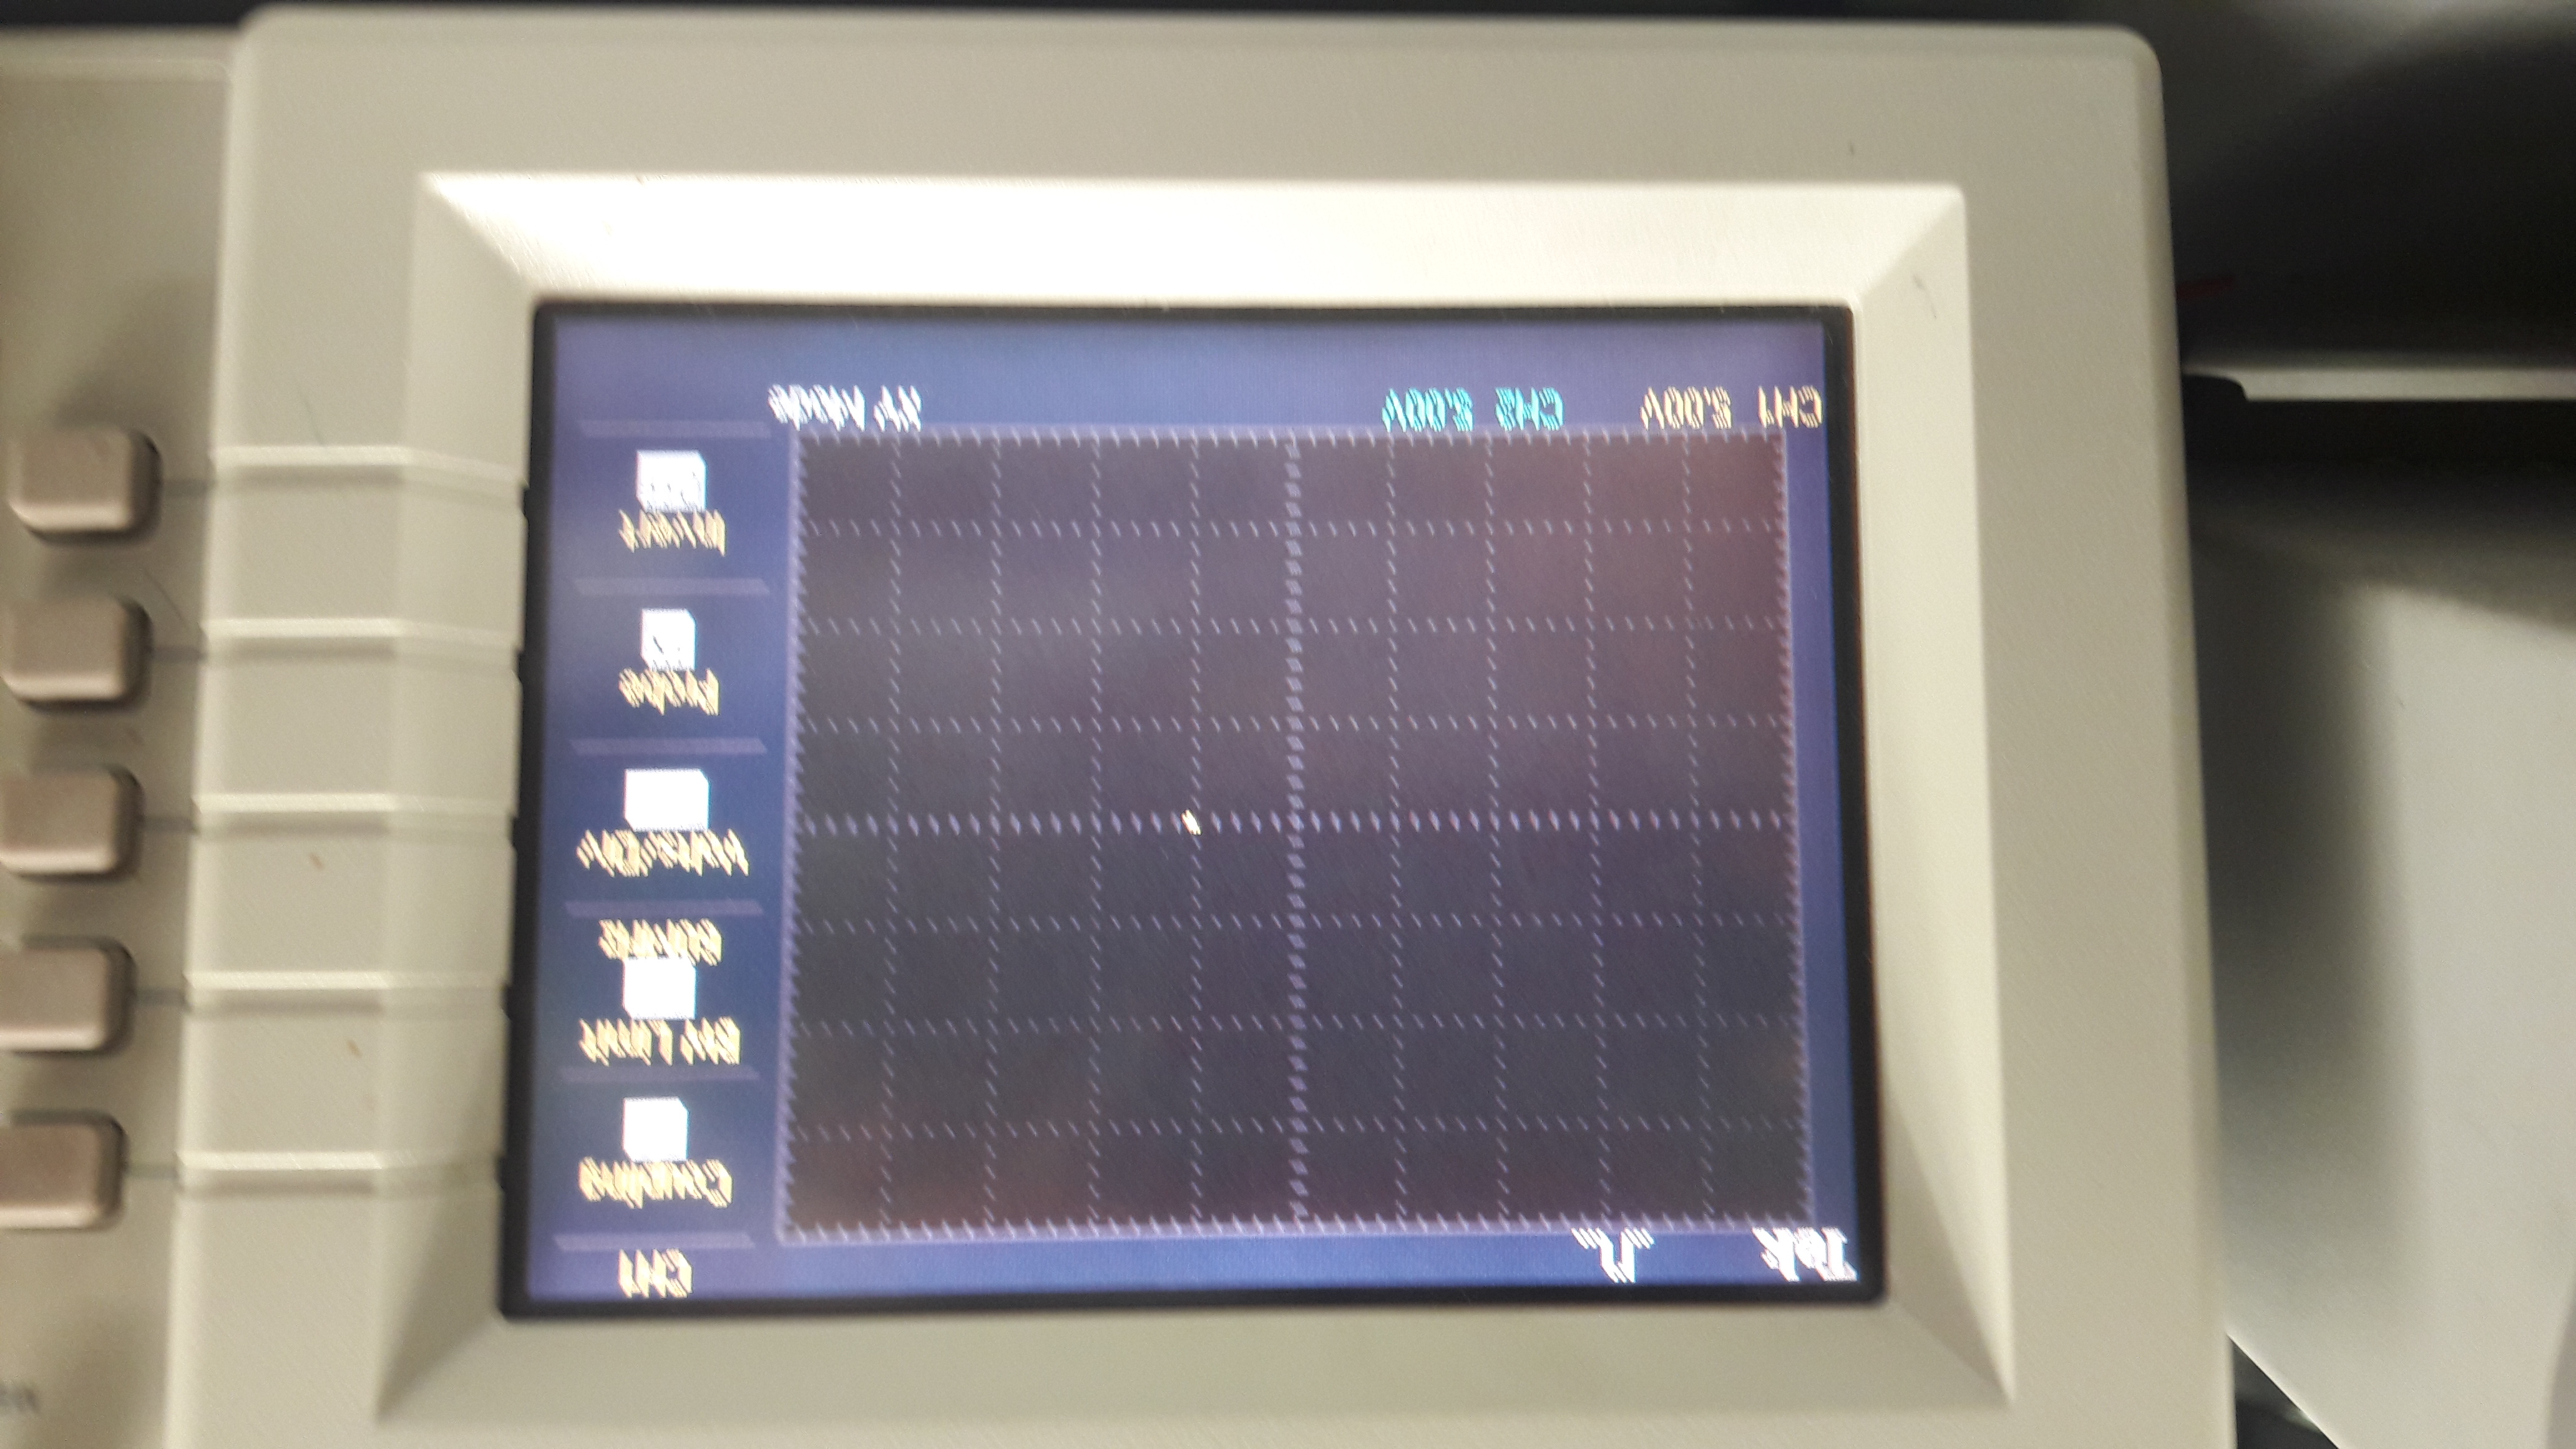
\includegraphics[width=.5\linewidth,angle=180]{img/part3/3}
    \caption{Oscilloscope with channels connected according to step 3}
\end{figure}
\begin{enumerate}
    \setcounter{enumi}{3}
\item Same connection but with channel Y inverted.
\end{enumerate}
%Tercera foto
\begin{figure}[H]
    \centering
    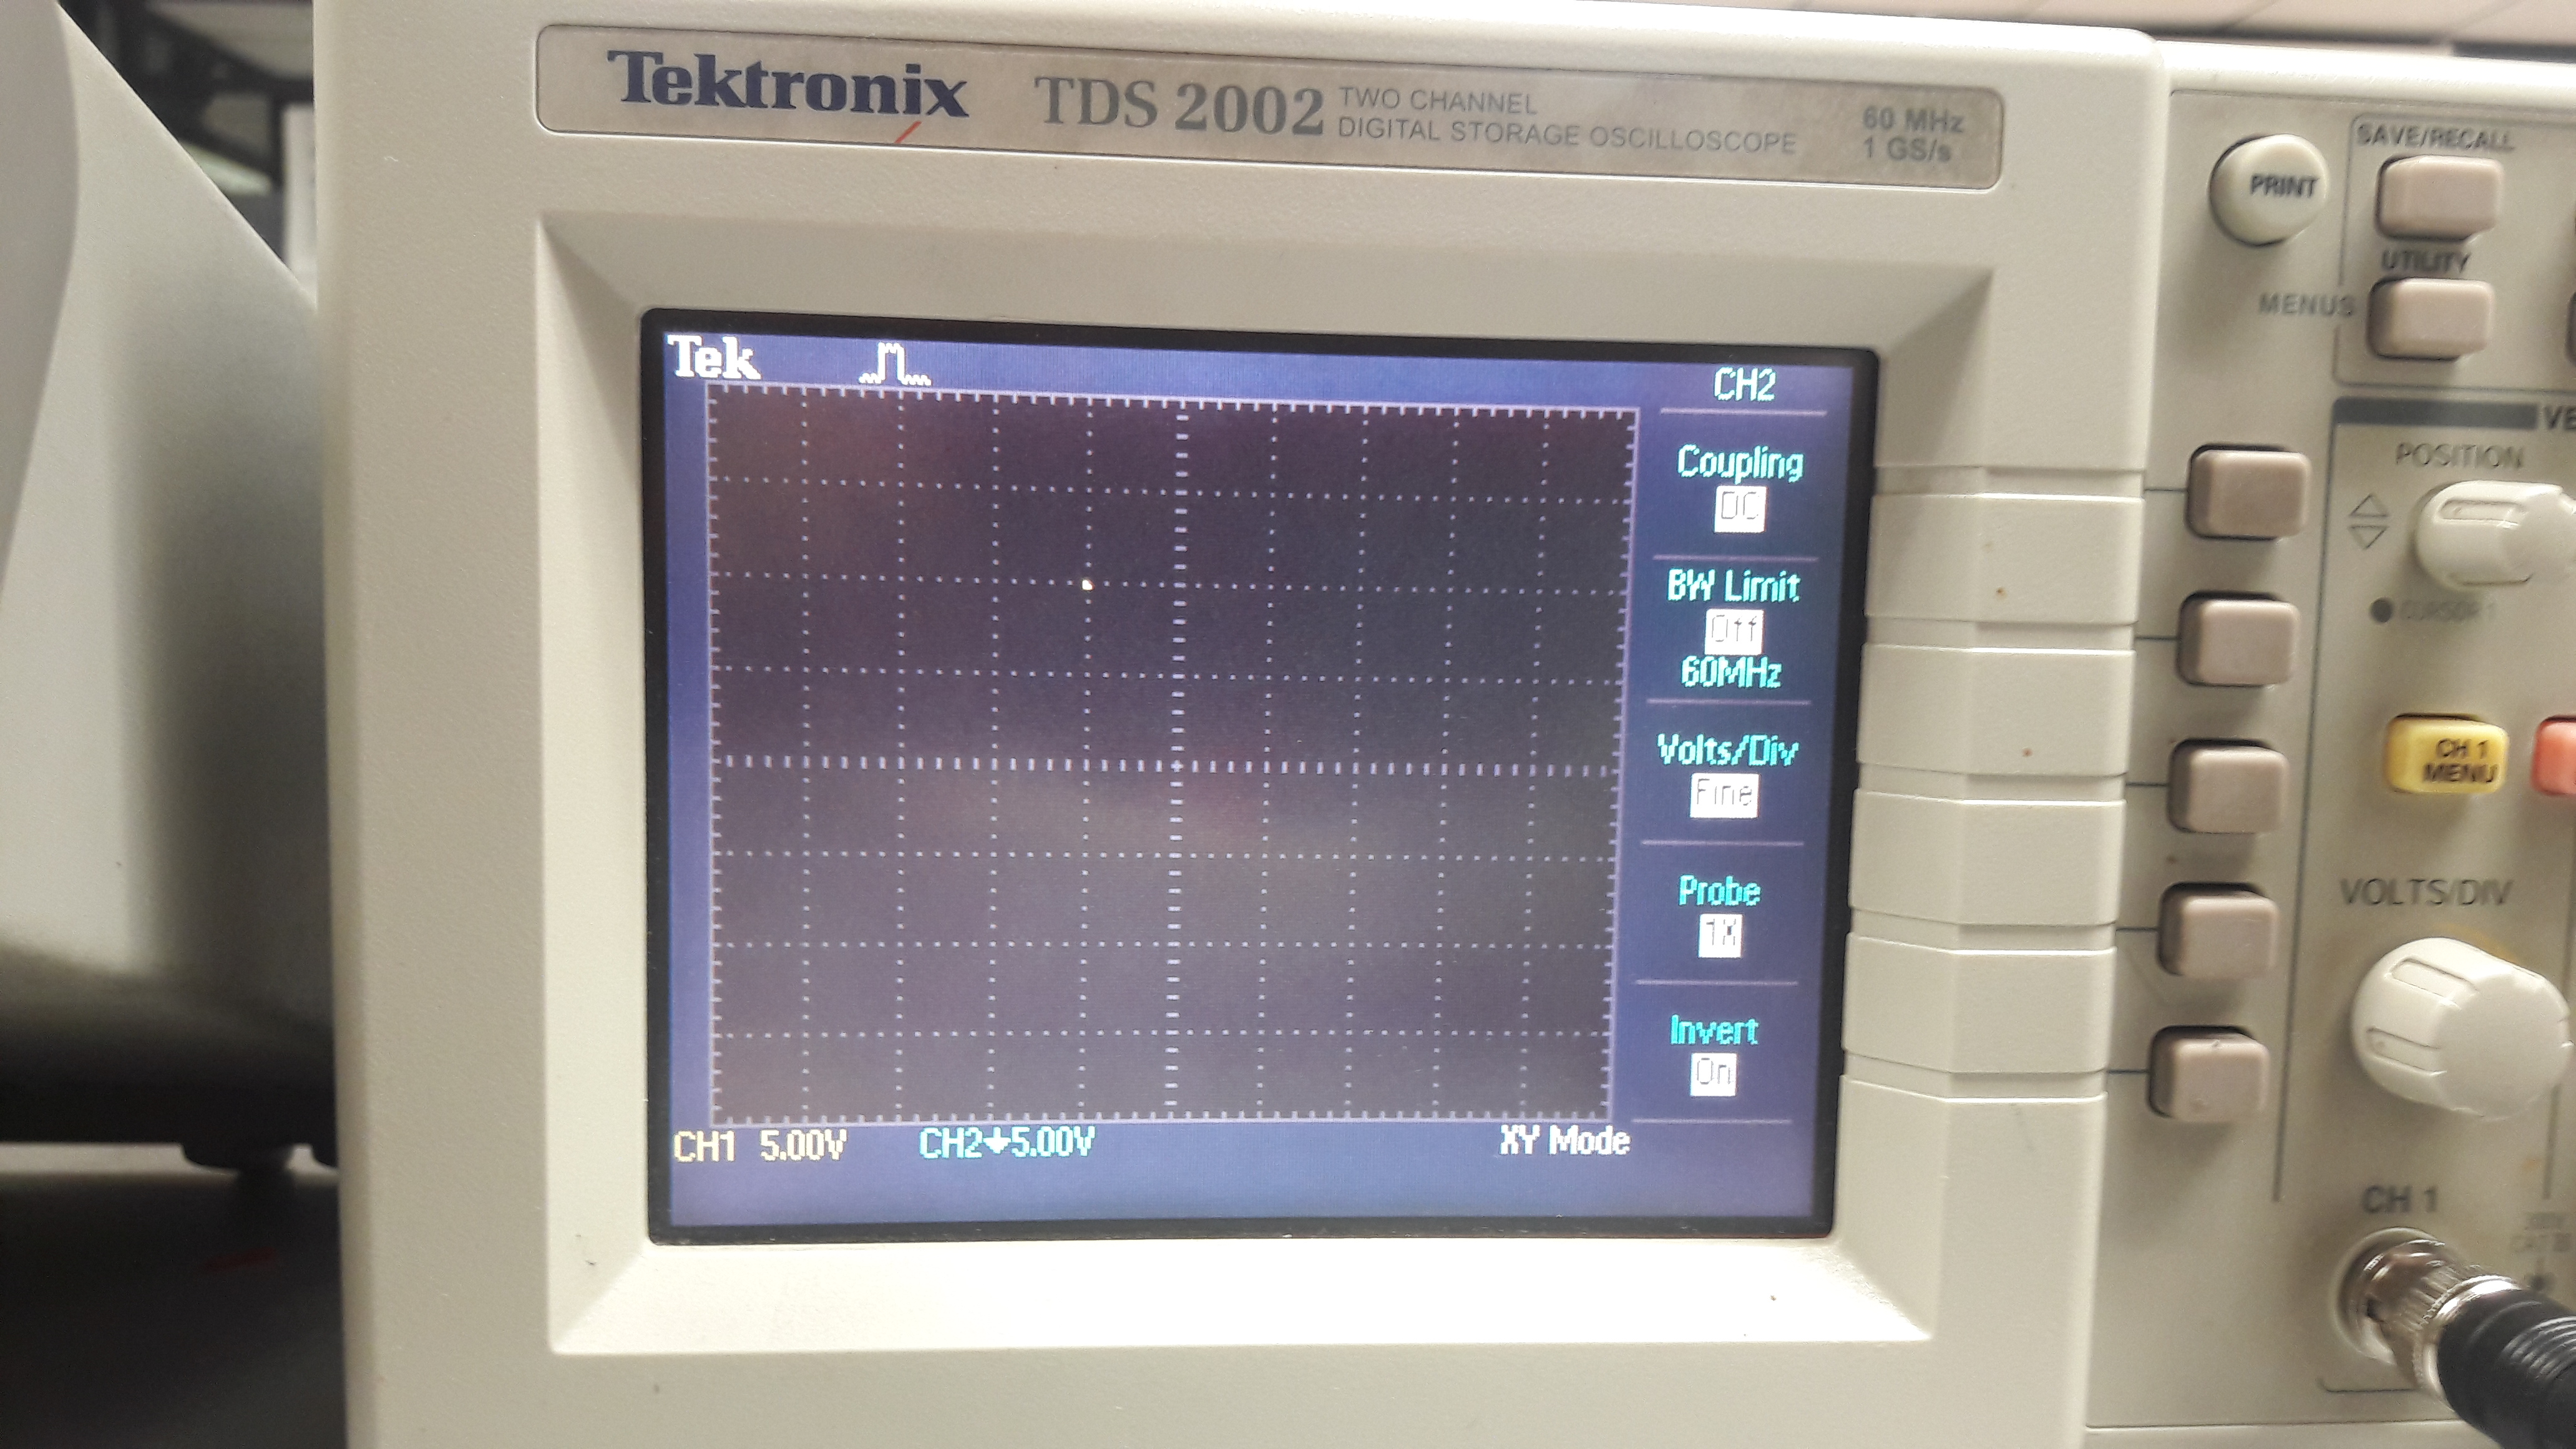
\includegraphics[width=.5\linewidth]{img/part3/5}
    \caption{Oscilloscope with channels connected according to step 4}
\end{figure}
\begin{enumerate}
    \setcounter{enumi}{4}
\item Positive of channel X to point B, positive of channel Y to point C, the negatives of both
channels to point A and Y channel inverted.
\end{enumerate}
%Cuarta foto
\begin{figure}[H]
    \centering
    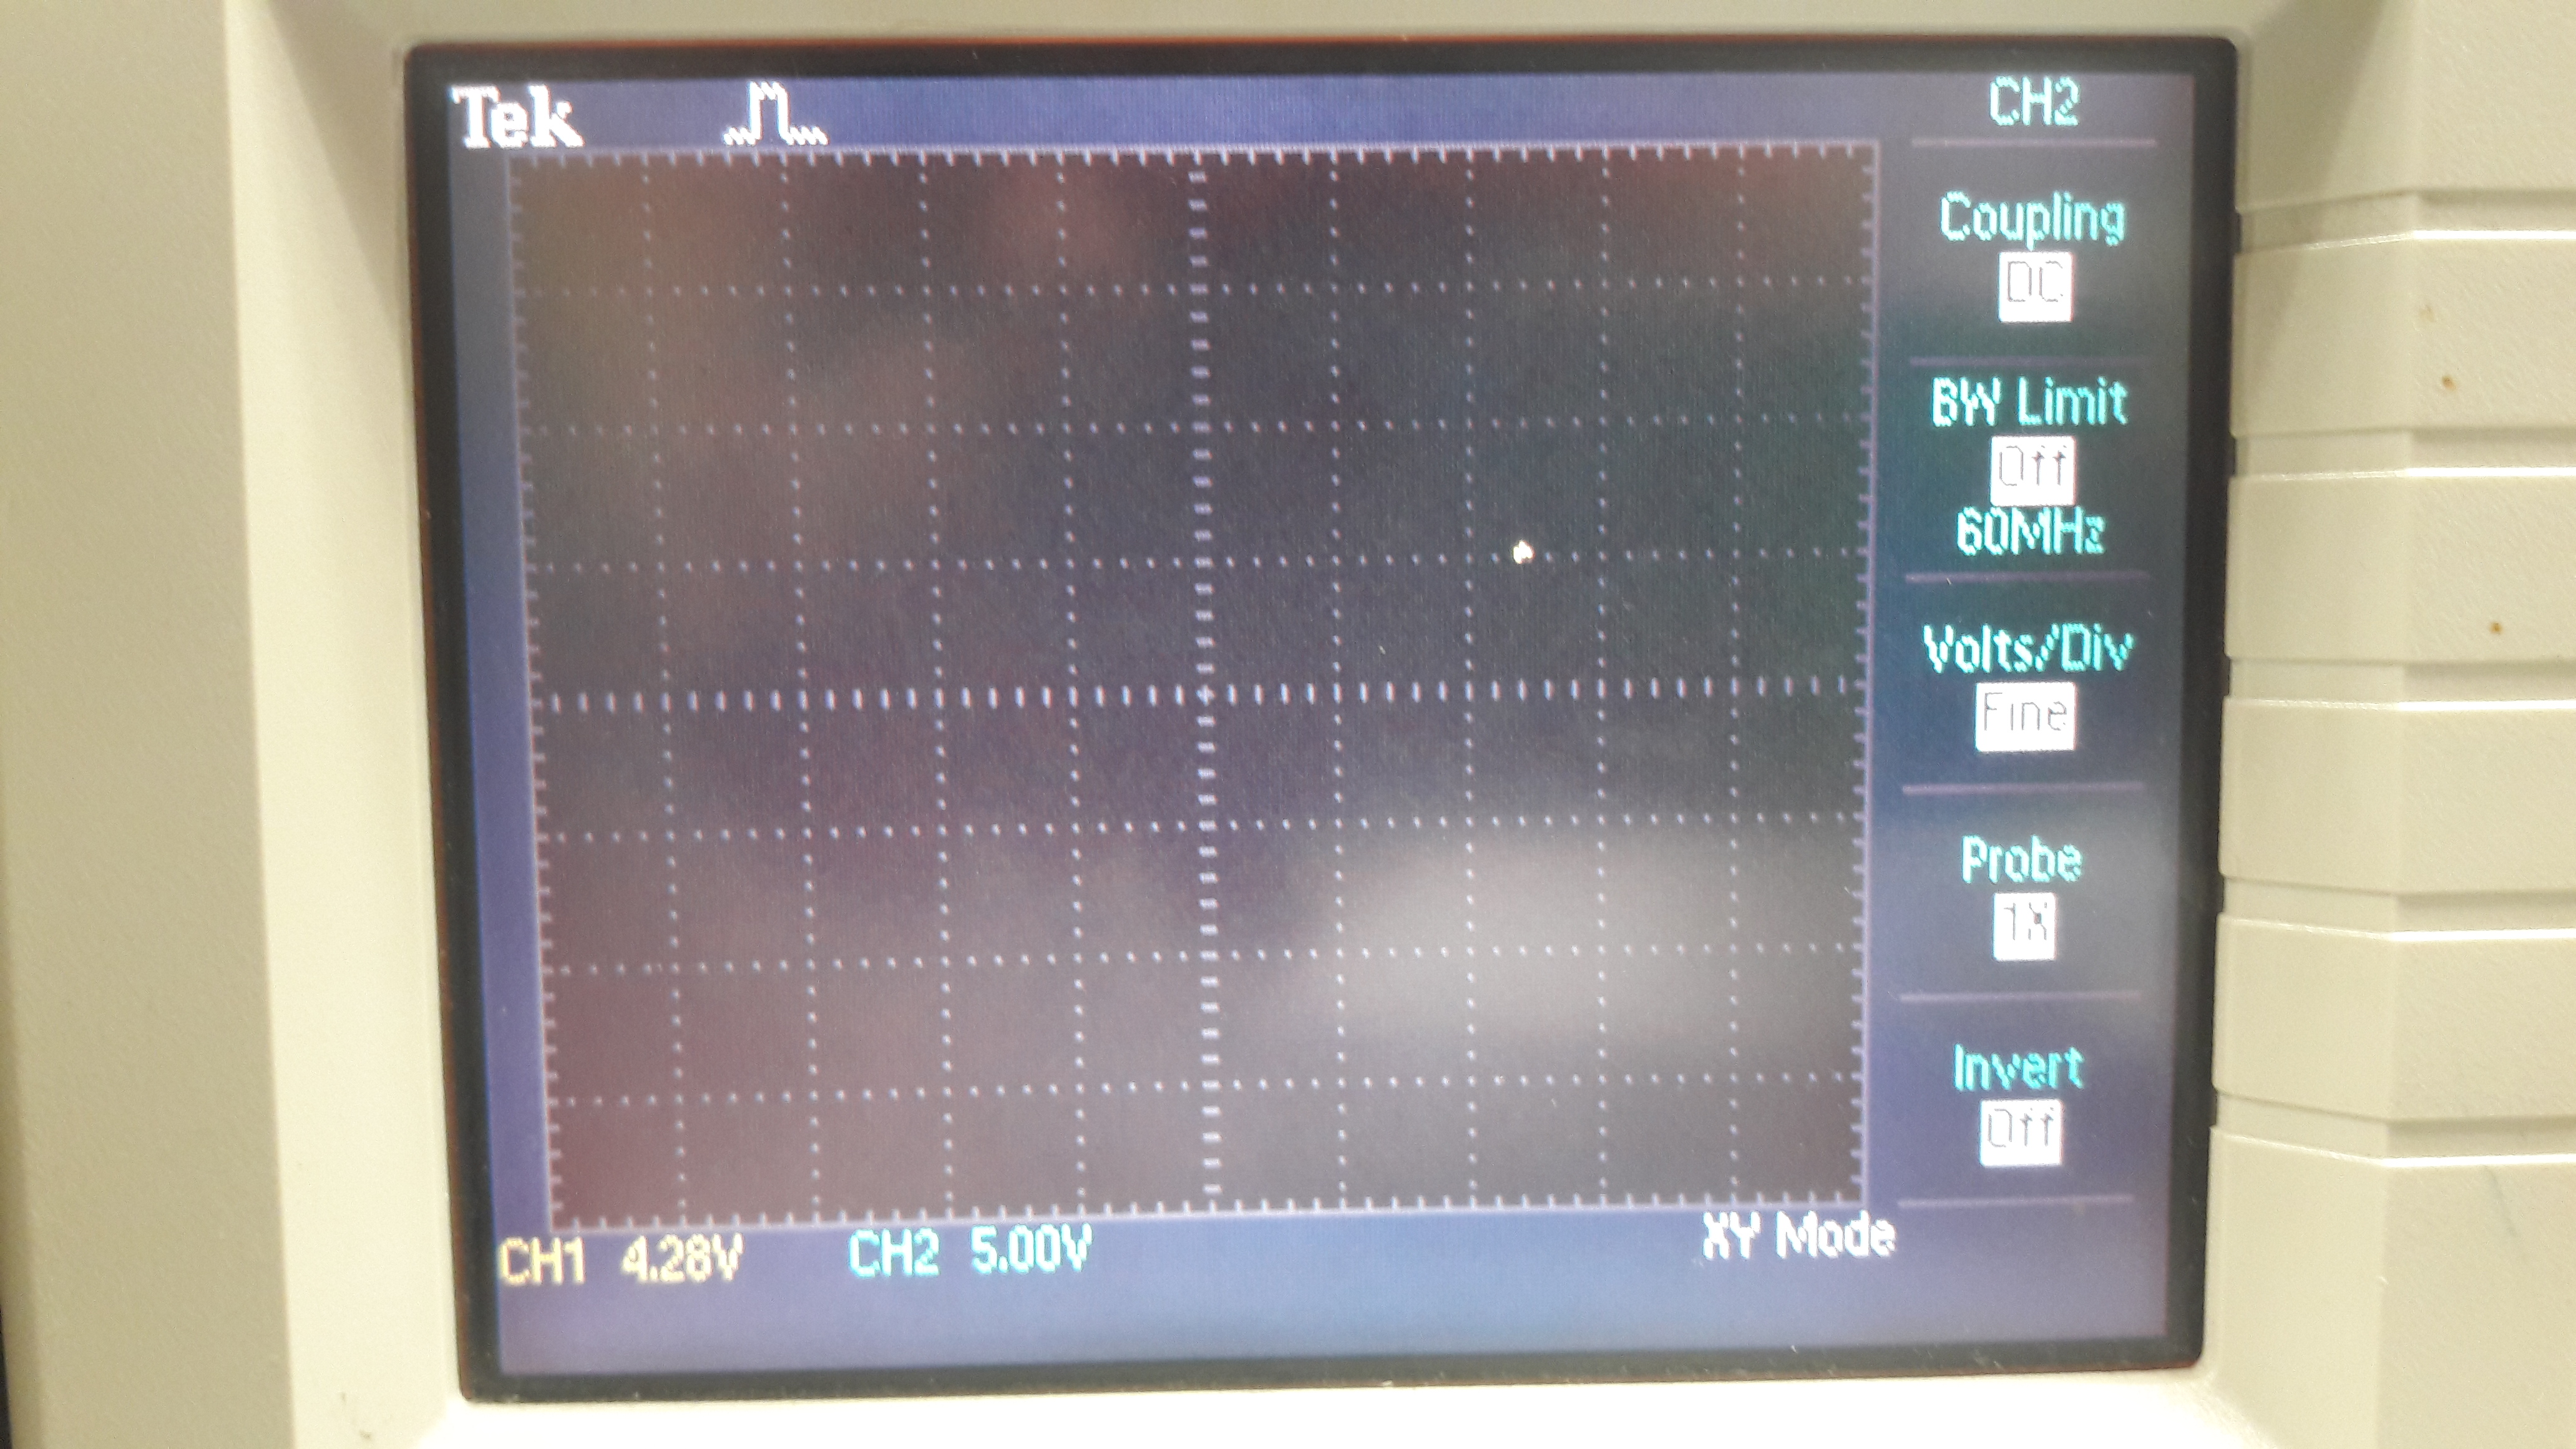
\includegraphics[width=.5\linewidth]{img/part3/1}
    \caption{Oscilloscope with channels connected according to step 4}
\end{figure}
\subsection{The oscilloscope as an X-Y plotter with AC currents}
In the last part of the experiment, we used the following circuit:
\begin{figure}[H]
    \centering
    \begin{circuitikz} \draw (3,4) -- (0,4) to [V=$10 V$,-] (0,0)
        (3,4) to [short,*-*] (6,4)
        (3,0) to [R=$\SI{10}{\kilo\ohm}$] (3,2)
        to [R=$\SI{10}{\kilo\ohm}$] (3,4)
        (3,2) to [short,*-*] (6,2)
        (0,0) -- (3,0) to [short,*-*] (6,0)
        {
            [anchor = south west](6,0) node {C}
            [anchor = south west](6,2) node {B}
            [anchor = south west](6,4) node {A}
        };
\end{circuitikz}
\end{figure}
then, with the oscilloscope set with AC coupling and Y(t) mode, we clipped the test probes to
their respective points according to the diagram shown before. After adjusting the size of each
graph, we could clearly see the phase shift between the graphs.
%!!!!Foto de fases
\subsubsection{Measurements}
\begin{figure}[H]
    \centering
    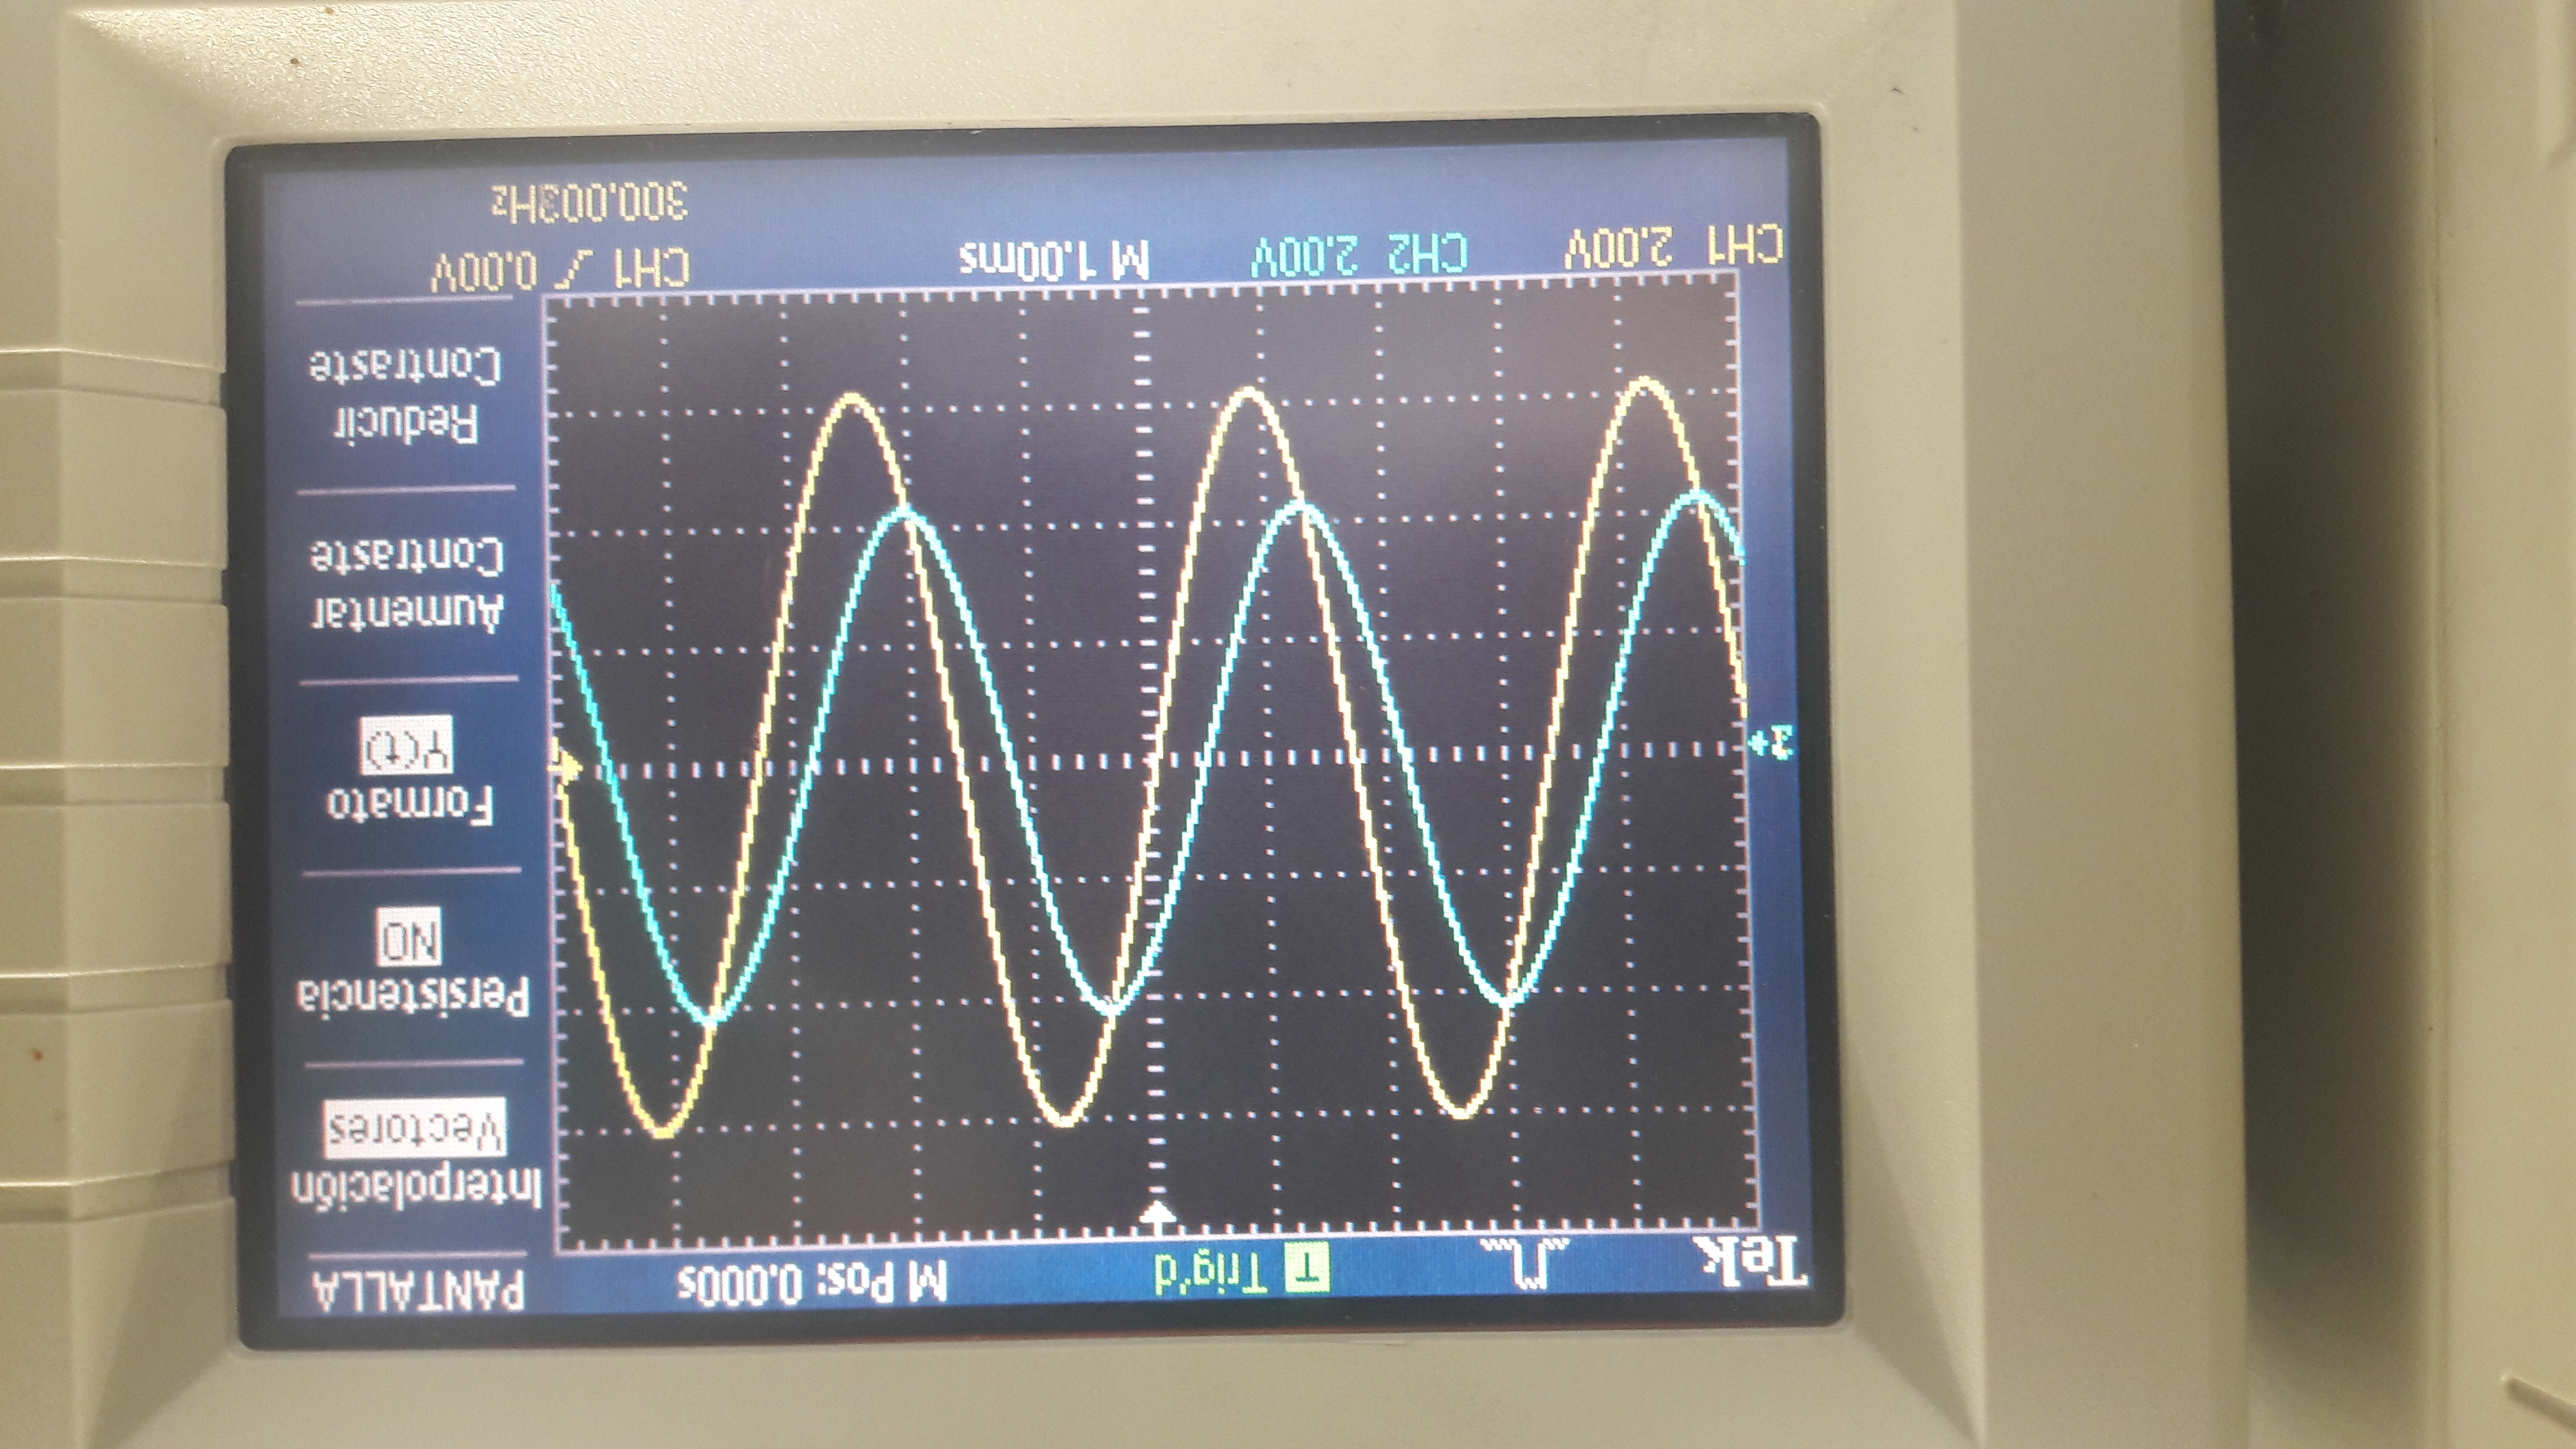
\includegraphics[width=.5\linewidth,angle=180]{img/part4/5}
    \caption{Oscilloscope showing the phase shift between the input and the output of the circuit
    using the $Y(t)$ mode}
\end{figure}
If phase shift($\phi$) is equal to:
\[\frac{(\ang{360})(a)}{T}\]
where $a$ is the time difference between the signals,we have that:
\begin{gather*}
    Volts/div = \SI{2}{\volt}\\
    Time/div = \SI{1}{\micro\second}\\
    a = \SI{3.2}{\second}
\end{gather*}
Therefore, phase shift($\phi$) is equal to:
\[\phi=\frac{(\ang{360})(\SI{0.4}{\second})}{\SI{3.2}{\second}}\qquad\therefore\phi=\ang{45}\]
Next, we changed to $X-Y$
mode, after adjusting voltage per division in both channels, we could spot a slightly rotated ellipse.
%!!!!!!!!Insertar fotos de elipse y curvas desfasadas
\begin{figure}[H]
    \centering
    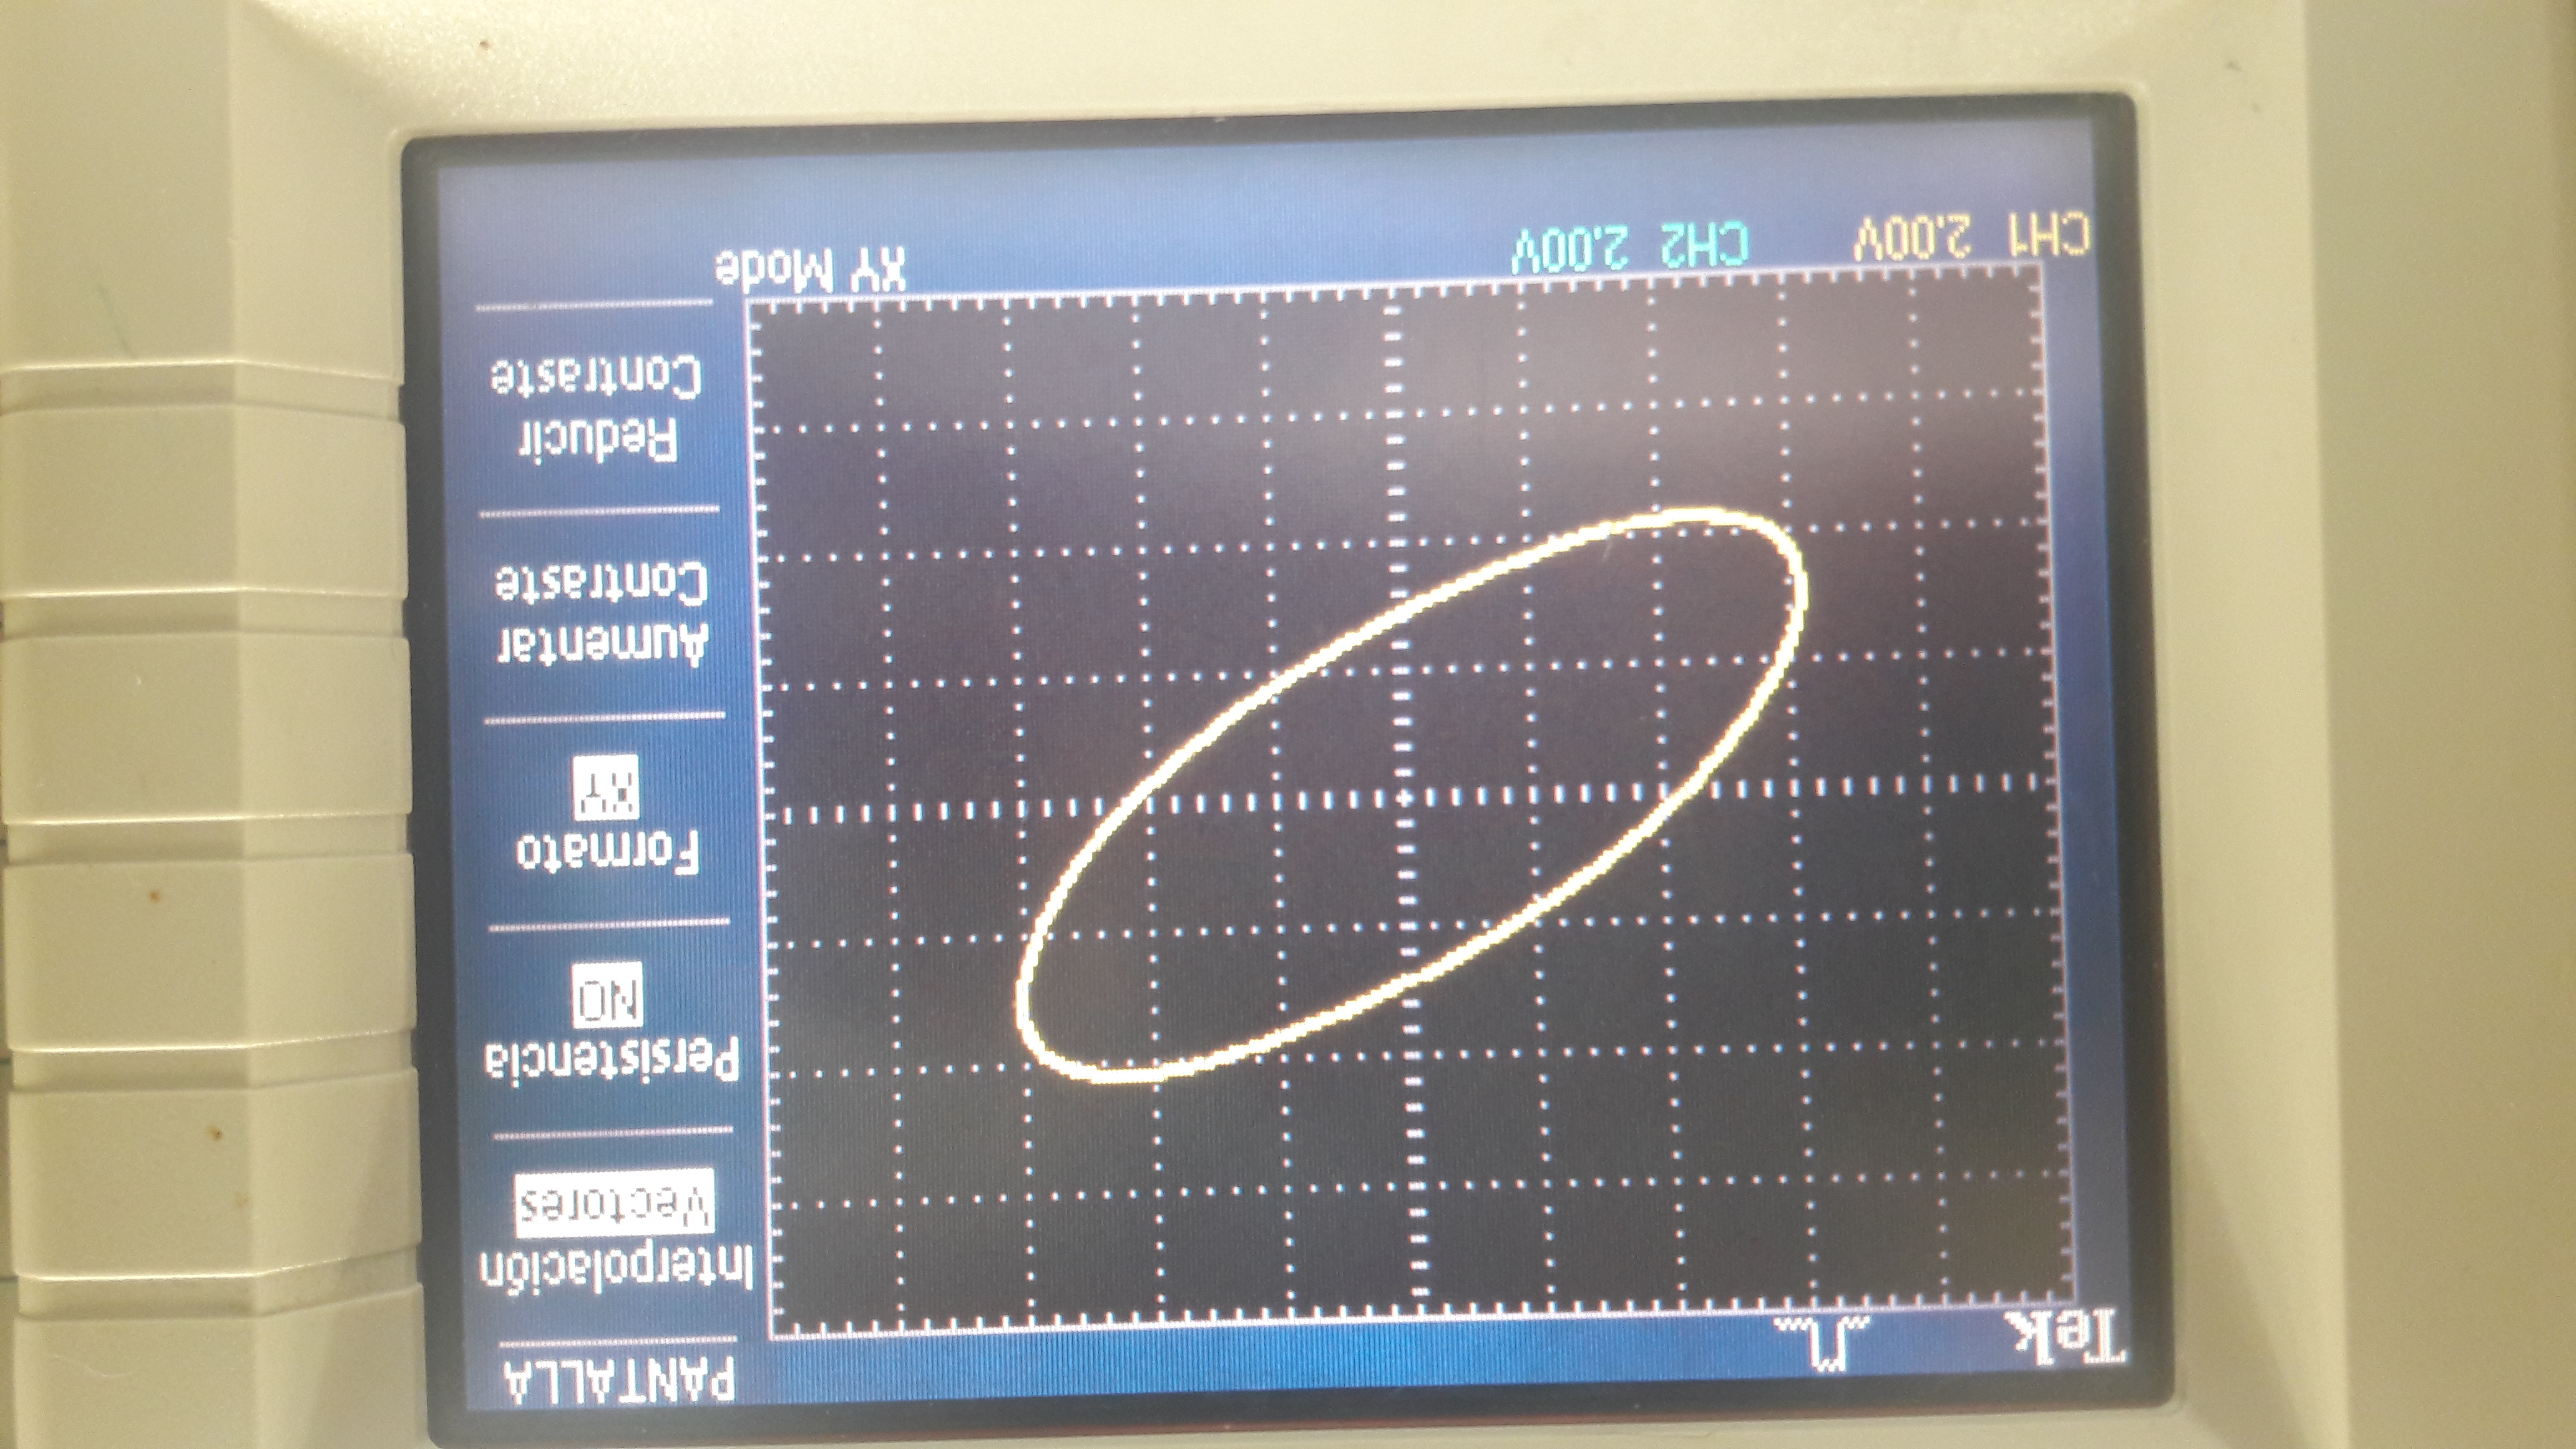
\includegraphics[width=.5\linewidth,angle=180]{img/part4/6}
    \caption{Oscilloscope showing the phase shift between the input and the output of the circuit
    using the $X-Y$ mode}
\end{figure}
Phase shift($\phi$) is given by:
\[\phi=\pm\sin^{-1}\Big(\frac{B}{A}\Big)\]
where $A$ is the y-coordinate of the peak of the ellipse in the first quadrant, and $B$ is the
y-coordinate where the ellipse intersects the x-axis, we have that:
\begin{gather*}
    Volts/div = \SI{2}{\volt}\\
    A = 1.5\\
    B = 2.1
\end{gather*}
Therefore, phase shift($\phi$) is equal to:
\[\phi=\pm\sin^{-1}\Big(\frac{1.5}{2.1}\Big)\qquad\therefore\phi=\ang{45.584}\]
\section{Questions}
\textit{\textbf{Explain the operation of the oscilloscope}}\\
To operate the oscilloscope we have to put to work the plates of vertical and horizontal deflection
\begin{figure}[H]
    \centering
    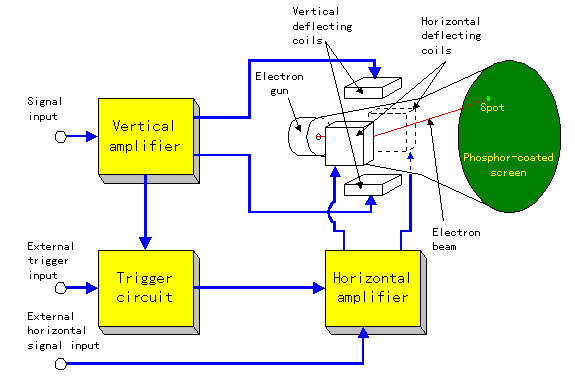
\includegraphics[width=.4\linewidth]{img/intro/diagram}
    \caption{Diagram of the oscilloscope}
\end{figure}
When the probe is connected to a circuit, the signal goes through the latter and goes to the vertical section. Depending on where we place the vertical amplifier control, we will attenuate the signal or amplify it.

At the exit of this block there is already enough signal to attack the vertical deflection plates (which are naturally horizontal) and are responsible for deflecting the electron beam, which emerges from the cathode and impacts the fluorescent layer inside the screen, vertically. Up if the tension is positive with respect to the reference point (GND) or down if it is negative.

The signal also goes through the firing section to start the horizontal sweep (this is responsible for moving the electron beam from the left side of the screen to the right side in a certain time).

The tracing (travel from left to right) is achieved by applying the ascending part of a saw tooth to the horizontal deflection plates (which are in vertical position), and can be adjustable in time by acting on the TIME-BASE knob. Retraction (travel from right to left) is done much faster with the descending part of the sawtooth itself.

In this way, the combined action of horizontal tracing and vertical deflection traces the graph of the signal on the screen. The firing section is necessary to stabilize the repetitive signals (it is ensured that the trace starts at the same point of the repetitive signal).

\textit{\textbf{What's the function of the signal generator?}}\\
A signal Generator is an electronic device that produces sinusoidal, square and triangular waves, as well as creating TTL signals. Its applications include testing and calibration of audio, ultrasonic and servo systems.
This function generator, specifically works in a frequency range between 0.2 Hz to 2 MHz. It also has a sweep function which can be controlled both internally and externally with a DC level. The machine cycle, DC offset level, sweep range and the width and width of the sweep can be controlled by the user.

\textit{\textbf{What are the Lissajous graphs for?}}\\
The Lissajous figures are used to determine the frequency and relative phase between two sinusoidal oscillations.
When an ascending diagonal to the right is obtained, it means that both frequencies are equal and in phase.
When an ascending diagonal to the left is obtained, it means that both frequencies are equal, but in phase opposition (180º angle).
When a circumference is obtained, it means that both frequencies are equal but offset by a right angle (90º).

\textit{\textbf{What are the operating modes Y (t) and XY used for?}}\\
There are vertical and horizontal amplifiers coupled to the aforementioned vertical and horizontal
deflection plates. In its most usual mode of operation, the waveform under study is applied to the
vertical input terminals. The vertical amplifier increases the amplitude sufficiently to cause an
appreciable vertical deflection of the electronic beam. The horizontal deviation of the beam is
achieved with a sweep generator, which is generally called "time base". Its mission is to elaborate
tensions in "sawtooth" that are those that "move" the beam horizontally. If the period of the signal
to be studied (vertical) is the same as the signal elaborated by the "time base", the image on the
screen appears "fixed". Figure 2 shows in the upper part (curve a), the periodic variations in time
of a voltage of period T, applied to the vertical deflection plates, i.e. Y = Y (t). In the horizontal deflection plates, the sweep generator supplies a sawtooth signal with the same period T (curve b), that is, X = X (t). To achieve a stable image, the time base must trigger "synchronously" with the signal to be measured. Sometimes this is done by deriving a trigger pulse from the amplified vertical signal to the sweep generator and other times it is convenient to trigger the sweep generator with an external signal
\begin{figure}[H]
    \centering
    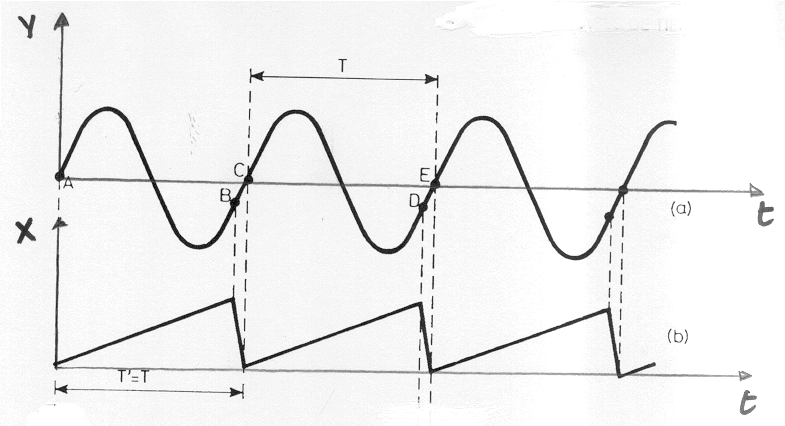
\includegraphics[width=.4\linewidth]{img/intro/waves}
    \caption{Individual signals for $X$ and $Y$ channel}
\end{figure}
The oscilloscope also allows to visualize the composition of two signals introduced by the two input channels and, in this case, it is said that the oscilloscope is operating in X-Y mode. Applying sinusoidal functions to both channels, the X-T mode would display two sine-type functions on the screen, while in X-Y mode an ellipse would be obtained on channel II.


\textit{\textbf{Which means by coupling in D.C.?}}\\
That when the DC coupling configuration provides a direct electrical path in the scope of application; It accepts all kinds of signals, including DC voltages that do not change, the DC voltages variable in time, AC, and combinations of AC and DC. In the latter case, technicians call an AC signal with a DC offset. Sometimes, CC offsets can be annoying; The voltage of the total signal can push the signal beyond the top or bottom of the screen, hiding the parts you want to see. However, in most other circumstances, DC coupling is all you need.

\textit{\textbf{What is an offset signal?}}\\
The offset of an alternating signal can be defined as the level of continuous that adds to an alternating signal. Thus, if the signal is centered at the origin, it is said that the offset level is 0. If it is displaced upwards, the offset is positive, whereas if it is displaced downwards, it will be negative.

Using the offset adjustment control, you can control the offset level that is added to the alternating signal of the function generator. Turning clockwise varies the offset positively and counterclockwise negatively.

\textit{\textbf{Which means that a signal is out of phase?}}\\
When two sinusoidal signals of the same frequency are compared, it may happen that both are not in phase, that is, the steps by equivalent points of both signals do not coincide in time. In this case it is said that both signals are out of phase, being able to measure the phase shift with a simple rule of three:
Being t the delay time between one signal and another.

\section{Conclusions}
{\large Sabrina:}\\
Oscilloscopes are utilized by everybody from TV repair professionals to physicists. They are key for
anybody planning or repairing electronic gear. The helpfulness of an oscilloscope is not constrained
to the universe of hardware. With the correct transducer, an oscilloscope can quantify a wide range
of wonders. Therefore, this tool has a very high importance for the engineer
\\[2ex]
{\large Salvador:}\\
In this practice, the oscilloscope and the voltage signal generator were used. The use of them was
explained, in the oscilloscope the signal of adjustment was evaluated, as a function of the time,
after which the signal generator was used to measure them in an oscilloscope. A circuit was then
assembled and measured in $xy$ function.
\\[2ex]
{\large Sebastián:}\\
We learned to use a very important instrument for the analysis of both DC and AC circuits, which is
the oscilloscope. This instrument is specially important when analysing alternate current circuits,
which are the most common in the real world, because of the nature of said signals which vary between
time, contrary to the direct current circuits which are always constant, allowing us to see the
changes between time using one or two signals, see the form of the wave of a given signal, and
another useful graphic representations that aid the analysis of circuits. 
\end{document}
